This chapter presents the results of comparing the proposed no-communication algorithm with Tarry's algorithm, as well as analyzing Tarry's performance against its variants. We evaluate these approaches on different datasets, detailed in Section \ref{section_datasets}, to observe how distinct graph properties influence the efficiency of the solutions. Section \ref{section_result_no_comm} discusses the performance of the no-communication algorithms. Section \ref{section_result_tarry} then presents the analysis of Tarry's algorithm and its variants.

\section{Datasets for Algorithm Evaluation} 
\label{section_datasets}

This section describes the datasets used to evaluate the performance of the algorithms. The datasets consist of four classes of graphs:

\begin{itemize} 
    \item Perfect Mazes: The dataset of perfect mazes \cite{Naeem2021} is the same as the one used by \citen{Arthur2023} and includes 250 mazes for each of four sizes: 10x10, 20x20, 30x30, and 40x40.
    \item Random Trees: The dataset of random trees was generated using the $random\_$ $unlabeled\_tree$ method from NetworkX \cite{Hagberg2008}. This function generates an unlabeled tree uniformly at random using Wilf's algorithm \cite{Wilf1981}, resulting in 250 trees for sizes: 100, 250, 500, 1000, and 1500 nodes. The goal node was chosen by randomly selecting one of the leaf nodes. Compared to the perfect mazes, these trees tend to be less deep and broader.
    \item Barabási-Albert Graphs: The dataset of Barabási-Albert graphs was generated using the dual Barabási-Albert preferential attachment method \cite{Moshiri2018} from NetworkX, specifically $dual\_barabasi\_albert\_graph$ function. This method constructs a random graph by incrementally adding new nodes that connect to existing nodes with a higher degree \cite{Barabasi1999}. For this dual approach, at each step of edge addition for a new node, it can be chosen whether the node will connect with either $n_1$ or $n_2$ edges, determined by a probability $p$ for $n_1$ and $1-p$ for $n_2$. In our case, $n_1$ is 2, $n_2$ is 3, and $p$ is set to 0.2. This approach results in networks that exhibit a power-law degree distribution, distinguishing them from the other datasets. The dataset includes graphs of sizes 100, 250, 500, 1000, and 1500 nodes.
    \item Small-World Network: The Small-World Network dataset was generated using NetworkX's $navigable\_small\_world\_graph$ function \cite{Hagberg2008}. Nodes are organized in an $n \times n$ grid, where each node connects to its local neighbors. Additionally, each node has one long-range connection assigned with a probability inversely proportional to the manhattan distance, given by $d((i,j),(k,l)) = |k-i| + |l-j|$, raised to the power $-r$ \cite{Kleinberg2000}. In this dataset, $q$ is set to 1, meaning each node has one additional long-range connection, and $r$ is set to 2.5. This configuration creates graphs of sizes 100, 250, 500, 1000 and 1500 nodes.
\end{itemize}

The sizes were chosen to approximately match the maze sizes used in \citen{Arthur2023} and to ensure that the computational demands for running all experiments remained manageable. For example, a 40x40 maze has 1600 cells, so graph sizes such as 1500 nodes were selected to provide a comparable level of complexity while keeping the analysis feasible across multiple runs.

For all datasets, after generating the graphs, nodes that did not contribute new decisions— specifically, those with a degree of 2 —were contracted. This contraction involves adding an edge between the node's two neighbors and removing the node itself. In the case of a perfect maze, this effectively eliminates every corridor. This removal process conserves memory and processing time, thus enhancing exploration efficiency and analysis, which particularly relevant for larger datasets. However, this process was not applied to the perfect mazes dataset used by \citen{Arthur2023}, as doing so would alter the structure of the mazes and affect the calculation of metrics, hindering valid comparisons.

Each dataset has distinct characteristics that can significantly influence the performance of the evaluated algorithms. To illustrate these effects, we present two tables: Table \ref{tab:average_depth} shows the average depth, counting only meaningful choices, of a Depth-First Search (DFS) exploration for each generated graph, excluding cycles, while Table \ref{tab:average_leaf_nodes} displays the average number of leaf nodes resulting from the same DFS exploration.

Additionally, we include Table \ref{tab:nodes_after_contraction}, which shows the average number of nodes remaining after the contraction process for each dataset. This table provides further insight into the structure of the datasets post-contraction.

\begin{table}[H]
    \centering
    \caption{Average Depth of DFS Exploration for Each Dataset}
    \label{tab:average_depth}
    \begin{tabular}{|c|c|c|c|c|c|c|} 
        \hline
        \textbf{Dataset} & \textbf{10x10/100} & \textbf{250} & \textbf{20x20/500} & \textbf{30x30/1000} & \textbf{40x40/1500} \\ 
        \hline
        Perfect Mazes & 6.79 & - & 18.31 & 31.29 & 48.98 \\ 
        \hline
        Random Trees & 6.78 & 10.52 & 15.20 & 22.24 & 27.04 \\ 
        \hline
        Barabási-Albert & 10.69 & 21.17 & 33.65 & 57.04 & 66.10 \\ 
        \hline
        Small-World & 0.004 & 0.22 & 0.002 & 0.23 & 0.001
        \\
        \hline
    \end{tabular}
\end{table}

\begin{table}[H]
    \centering
    \caption{Average Number of Leaf Nodes for Each Dataset}
    \label{tab:average_leaf_nodes}
    \begin{tabular}{|c|c|c|c|c|c|} 
        \hline
        \textbf{Dataset} & \textbf{10x10/100} & \textbf{250} & \textbf{20x20/500} & \textbf{30x30/1000} & \textbf{40x40/1500} \\ 
        \hline
        Perfect Mazes & 11.58 & - & 41.88 & 92.58 & 162.14 \\ 
        \hline
        Random Trees & 34.76 & 85.64 & 172.22 & 345.41 & 516.53 \\ 
        \hline
        Barabási-Albert & 21.17 & 46.70 & 81.21 & 149.26 & 191.41 \\
        \hline
        Small-World & 1.01 & 1.22 & 1.00 & 1.23 & 1.00
        \\
        \hline
    \end{tabular}
\end{table}

\begin{table}[H]
    \centering
    \caption{Average Number of Nodes After Contraction for Each Dataset}
    \label{tab:nodes_after_contraction}
    \begin{tabular}{|c|c|c|c|c|c|} 
        \hline
        \textbf{Dataset} & \textbf{10x10/100} & \textbf{250} & \textbf{20x20/500} & \textbf{30x30/1000} & \textbf{40x40/1500} \\ 
        \hline
        Perfect Mazes & 100 & - & 500 & 1000 & 1500 \\ 
        \hline
        Random Trees & 51.26 & 124.56 & 251.03 & 502.02 & 752.89 \\ 
        \hline
        Barabási-Albert & 59.89 & 125.15 & 207.66 & 366.44 & 444.65 \\
        \hline
        Small-World & 98.26 & 223.41 & 482.296 & 959.528 & 1442.376
        \\
        \hline
    \end{tabular}
\end{table}

The results presented in the tables allow for a clear comparison of the datasets. The Barabási-Albert graphs exhibited the greatest average depth in the DFS exploration and the second highest number of leaf nodes, indicating their complexity. Notably, they were also the most affected by the contraction process, resulting in a significant reduction in node count. In contrast, the Random Trees dataset had the least depth and the highest average number of leaf nodes, showcasing its broader structure. Perfect Mazes, while exhibiting moderate depth and leaf nodes, did not undergo contraction, preserving their original node counts for valid metric comparisons.

The Small-World dataset exhibits unique characteristics in Tables \ref{tab:average_depth} and \ref{tab:average_leaf_nodes}, where average depth approaches zero and the number of leaf nodes remains near one. This occurs due to the DFS traversal's fixed search order (North, East, South, West, followed by any other connected node), producing a nearly linear, degenerate tree structure where each parent node has only one child. Corridor contraction further simplifies this structure, reducing the tree to a single node, hence the minimal depth and single leaf node. Although this pattern implies a single agent almost always can traverse the grid without backtracking, additional agents can still enhance performance by distributing across the grid while following different search orders, making this dataset suitable for our analysis.


\section{No-Communication Algorithms Performance}
\label{section_result_no_comm}

\subsection{Metrics for Analysis}
\label{subsection_no_comm_metrics}

This section focuses on the results for the zero-communication algorithms, which include the basic distributed search algorithm and its Backward Interval Filling variant. Tarry's algorithm is also included for comparison, despite involving communication. The reason for this choice is that zero-communication algorithms provide a lower limit for assessing the efficiency of any distributed search algorithm employing communication, and we aim to compare them with a communication-based approach like Tarry's.


The metrics used in this comparison are the same as those from \citen{Kivelevitch2010}:

\begin{itemize}
    \item Steps Taken by the Pioneer: This measures the number of steps needed by the first agent to find the goal, serving as a key indicator of exploration efficiency.
    \item Fraction Explored Before the Pioneer Found the Goal: This indicates the proportion of the graph explored by the agents when the goal is reached, providing insight into how well the agents dispersed during exploration.
\end{itemize}
    
These metrics together give a clear view of the algorithm's efficiency and how exploration patterns vary across different graph structures and sizes.

\subsection{Perfect Maze Results} 
\label{subsection_no_comm_maze_results}


The results for all maze sizes (10x10, 20x20, 30x30, and 40x40) are presented in Figures \ref{fig_no_comm_steps_all_sizes_maze} and \ref{fig_no_comm_fraction_all_sizes_maze}, showing how the different no-communication algorithms perform across various maze dimensions. Figure \ref{fig_no_comm_steps_all_sizes_maze} represents the steps taken by the pioneer, while Figure \ref{fig_no_comm_fraction_all_sizes_maze} shows the explored fraction before the goal was found, allowing for a detailed comparison of exploration efficiency and coverage.

\begin{figure}[H]
    \centering
    \qquad
    \qquad
    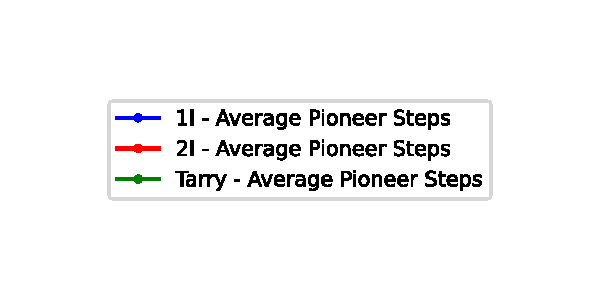
\includegraphics[width=0.5\textwidth]{Cap3/no_comm_steps_legend.pdf}
    \newline
    \subfloat[\centering 10x10 Maze]
    {{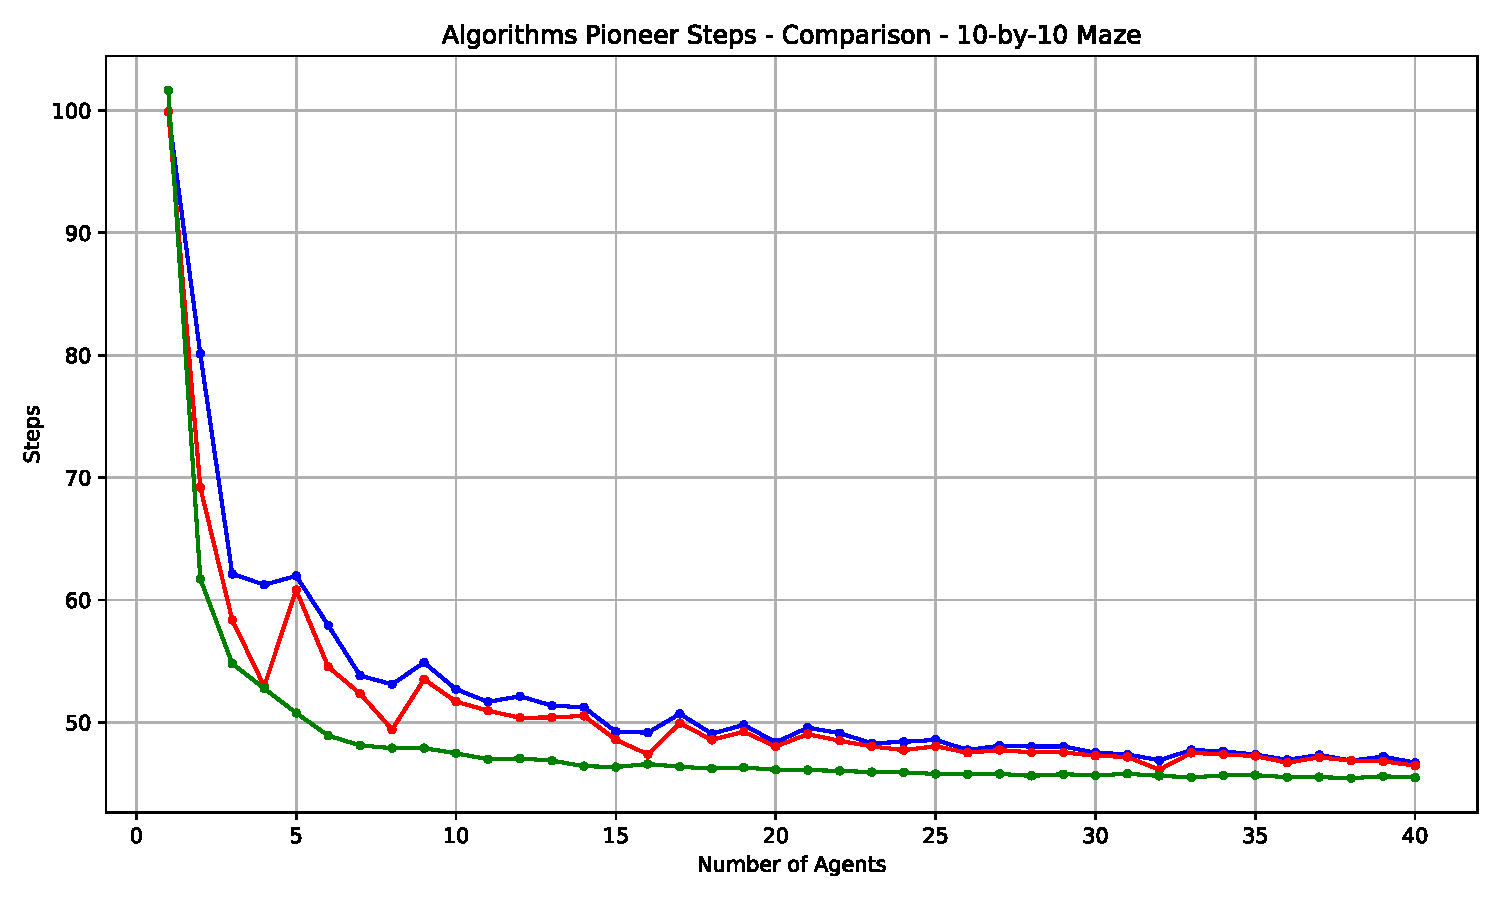
\includegraphics[width=0.45\linewidth]{Cap3/no_comm_steps__10_by_10_maze.pdf} }}
    \qquad
    \subfloat[\centering 20x20 Maze]
    {{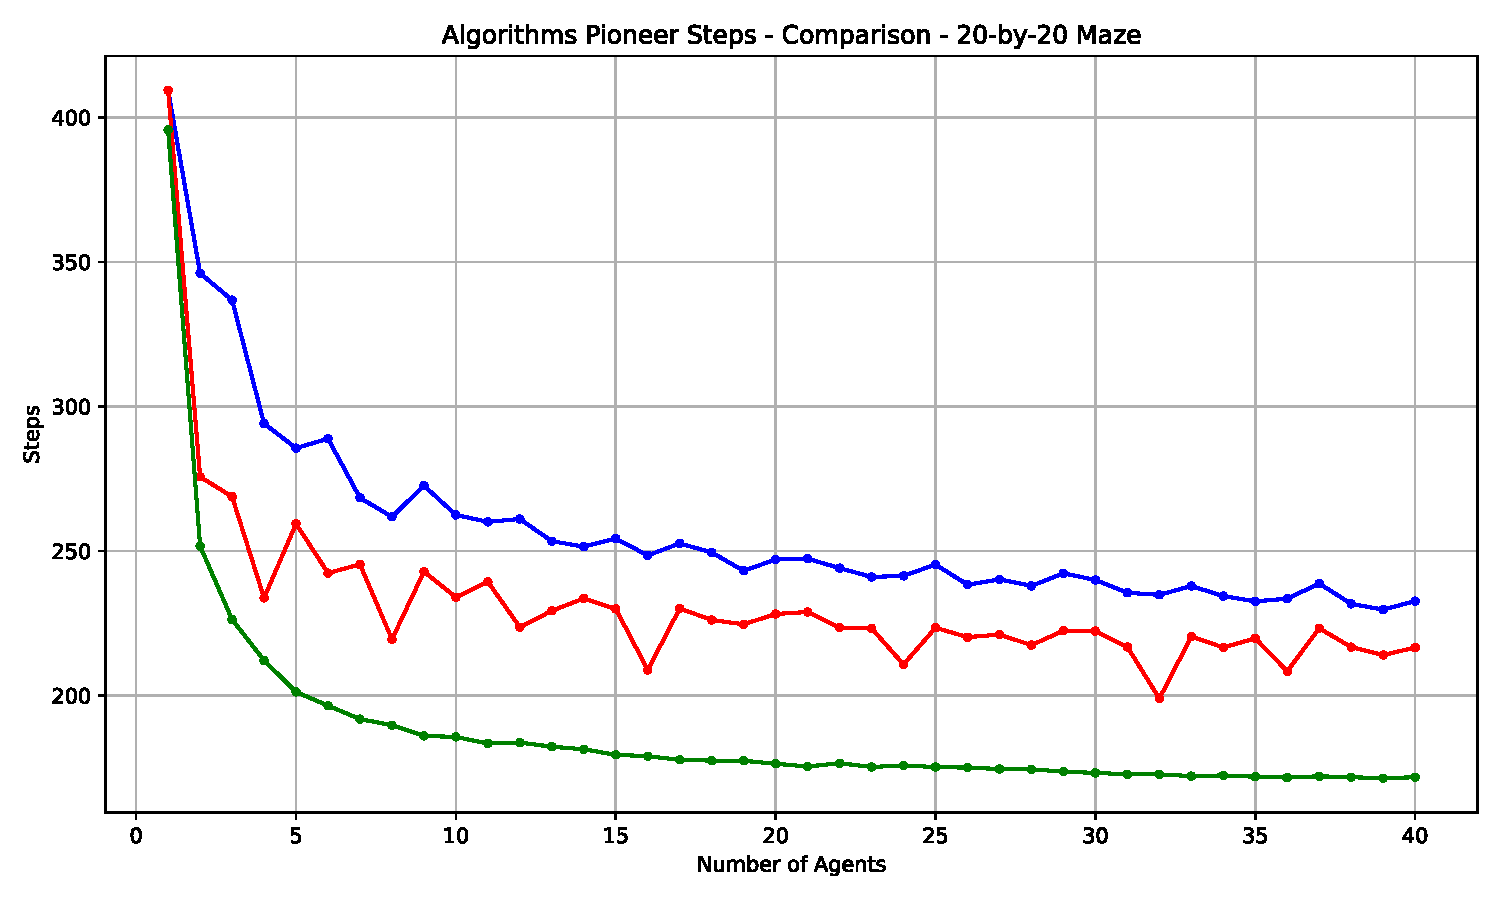
\includegraphics[width=0.45\linewidth]{Cap3/no_comm_steps__20_by_20_maze.pdf} }}
    \newline
    \subfloat[\centering 30x30 Maze]
    {{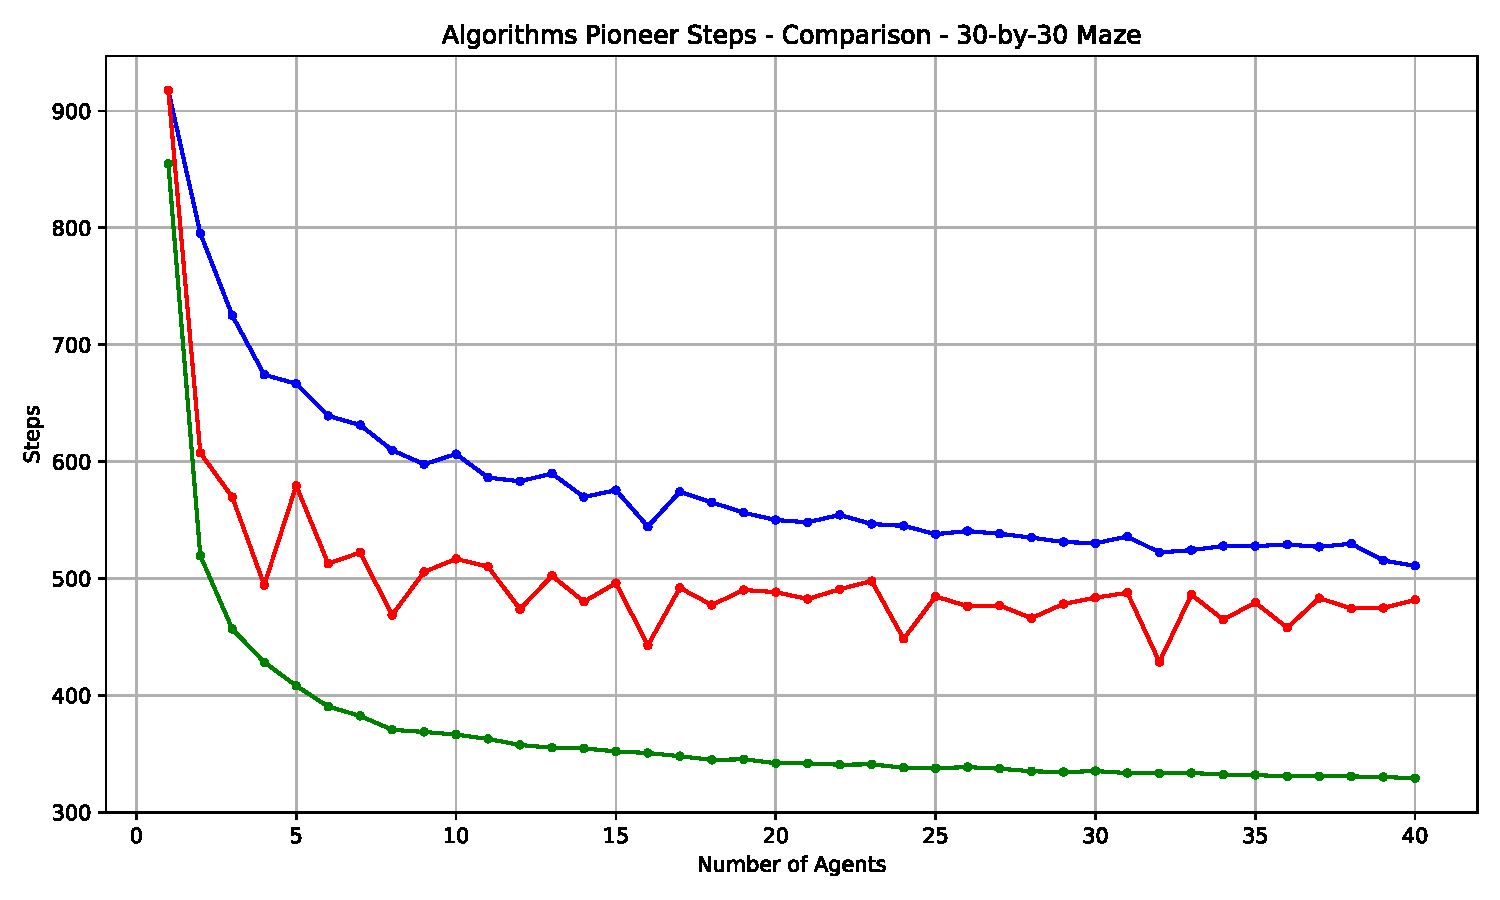
\includegraphics[width=0.45\linewidth]{Cap3/no_comm_steps__30_by_30_maze.pdf} }}
    \qquad
    \subfloat[\centering 40x40 Maze]
    {{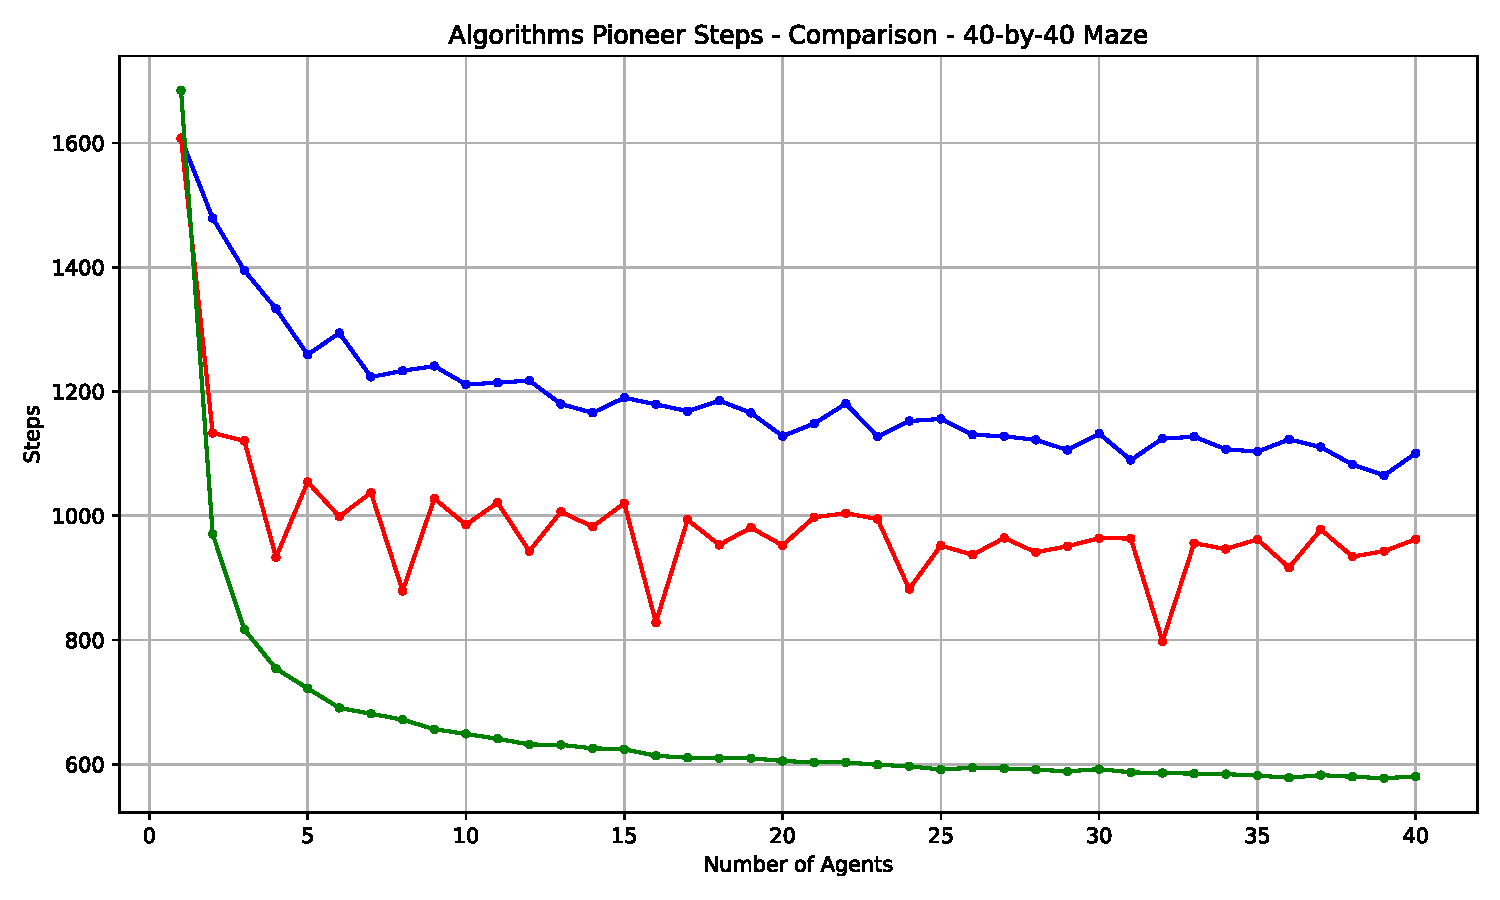
\includegraphics[width=0.45\linewidth]{Cap3/no_comm_steps__40_by_40_maze.pdf} }}
    \caption{Comparison of the pioneer's average steps between our no-communication algorithms and Tarry's algorithm across different sizes of perfect mazes. The subfigures illustrate how algorithm performance scales with maze size.}
    \label{fig_no_comm_steps_all_sizes_maze}
\end{figure}

\begin{figure}[H]
    \centering
    \qquad
    \qquad
    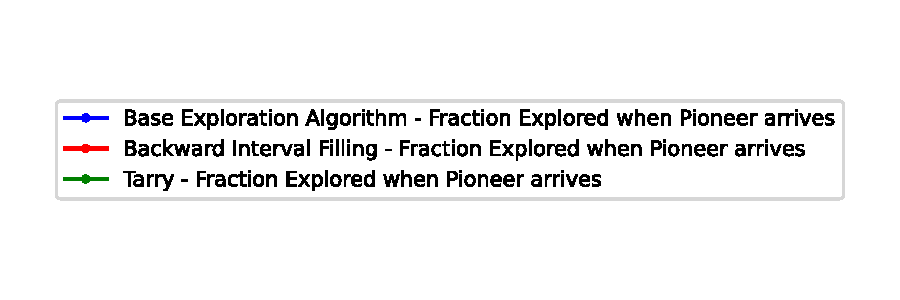
\includegraphics[width=0.5\textwidth]{Cap3/no_comm_fraction_legend.pdf}
    \newline
    \subfloat[\centering 10x10 Maze]
    {{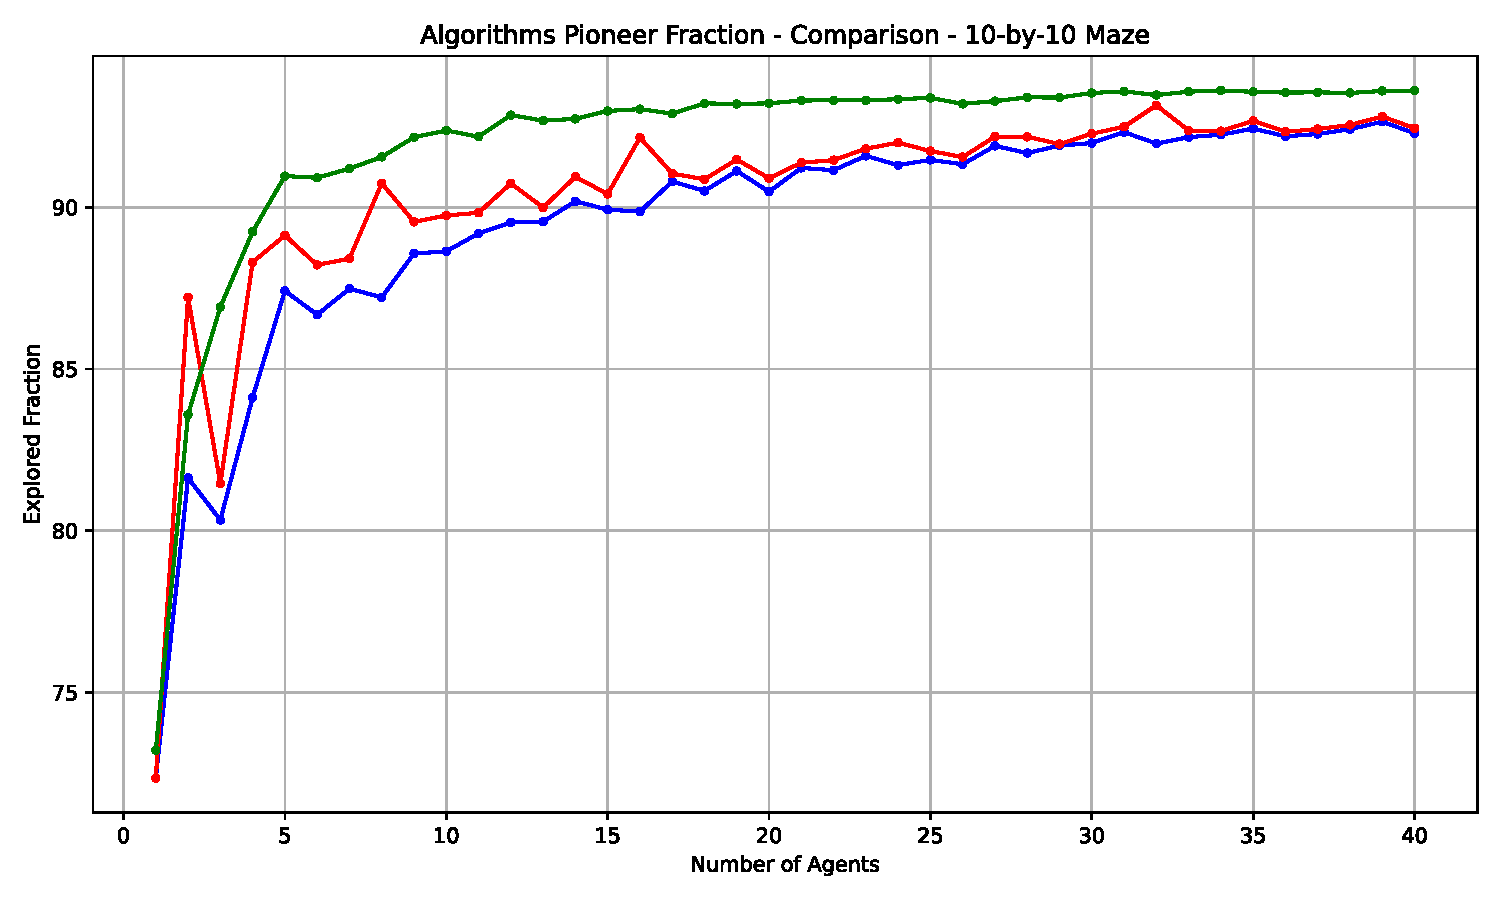
\includegraphics[width=0.45\linewidth]{Cap3/no_comm_fraction__10_by_10_maze.pdf} }}
    \qquad
    \subfloat[\centering 20x20 Maze]
    {{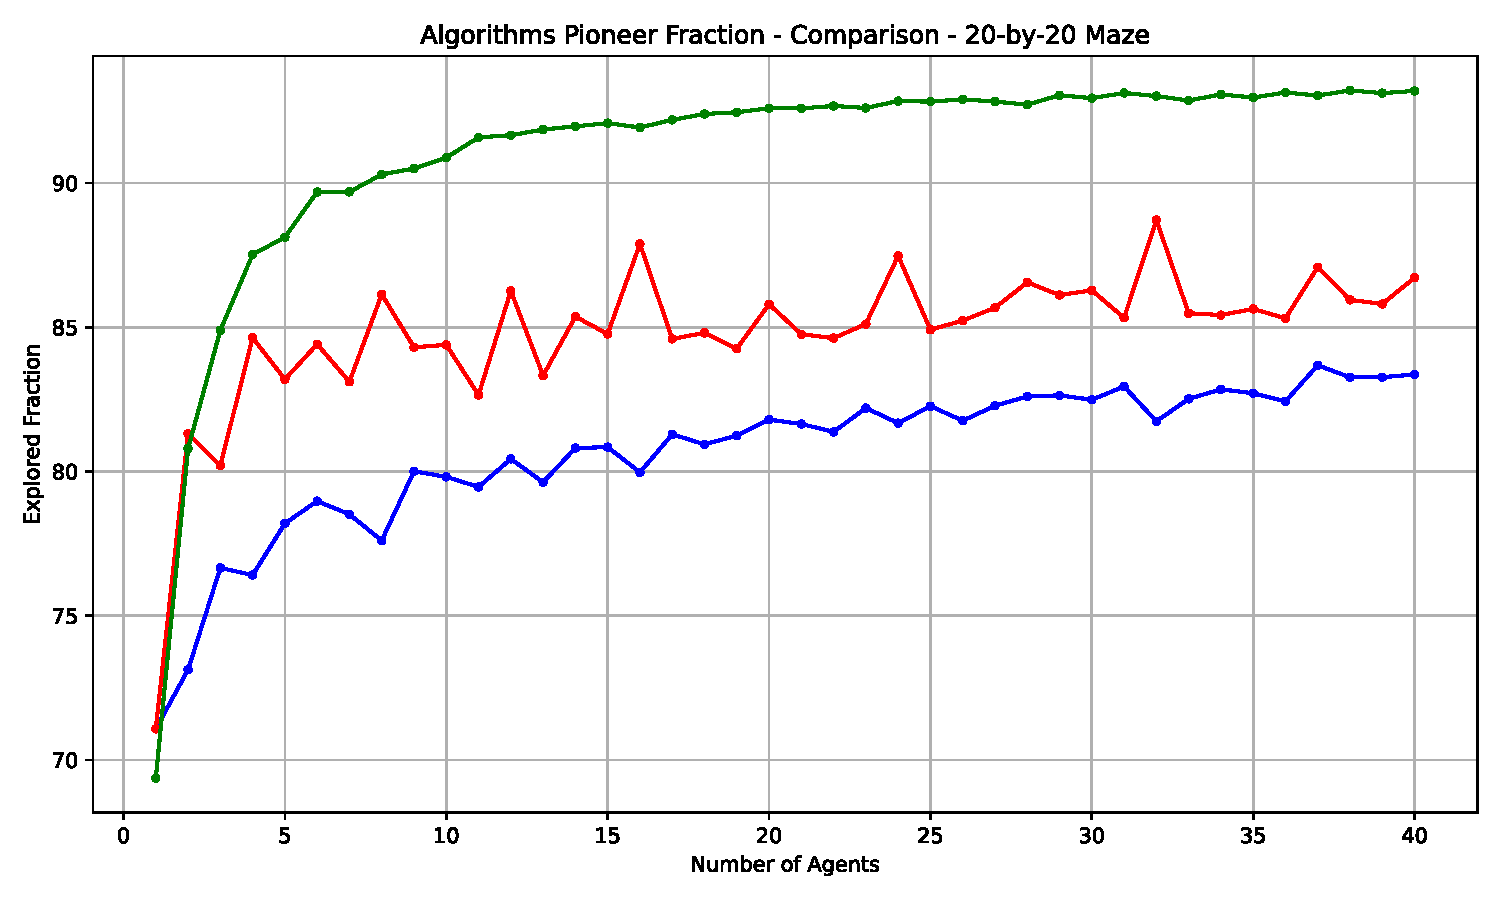
\includegraphics[width=0.45\linewidth]{Cap3/no_comm_fraction__20_by_20_maze.pdf} }}
    \newline
    \subfloat[\centering 30x30 Maze]
    {{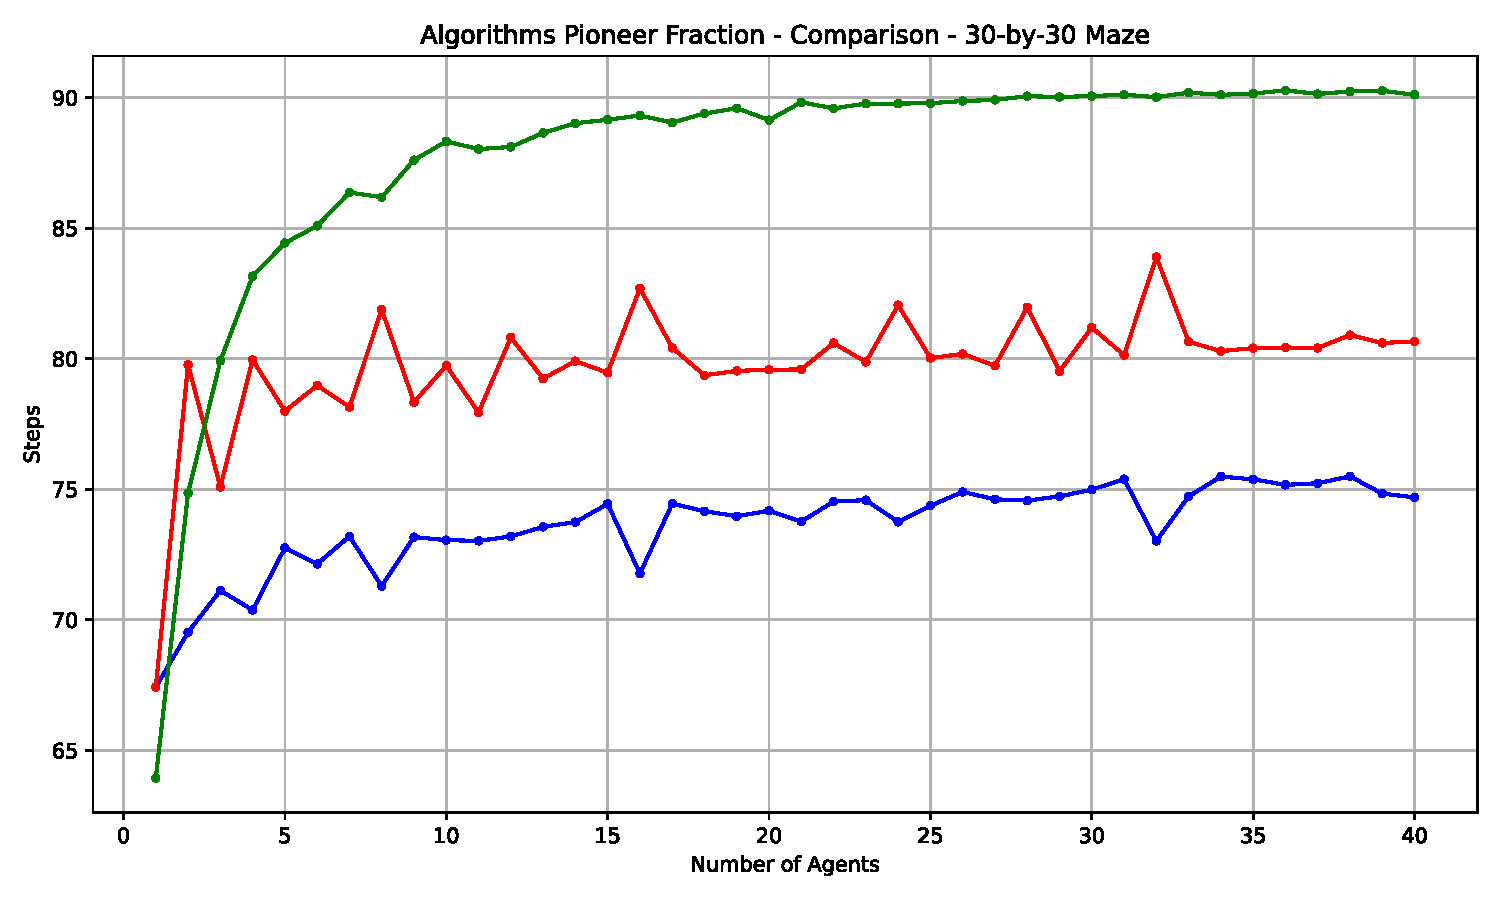
\includegraphics[width=0.45\linewidth]{Cap3/no_comm_fraction__30_by_30_maze.pdf} }}
    \qquad
    \subfloat[\centering 40x40 Maze]
    {{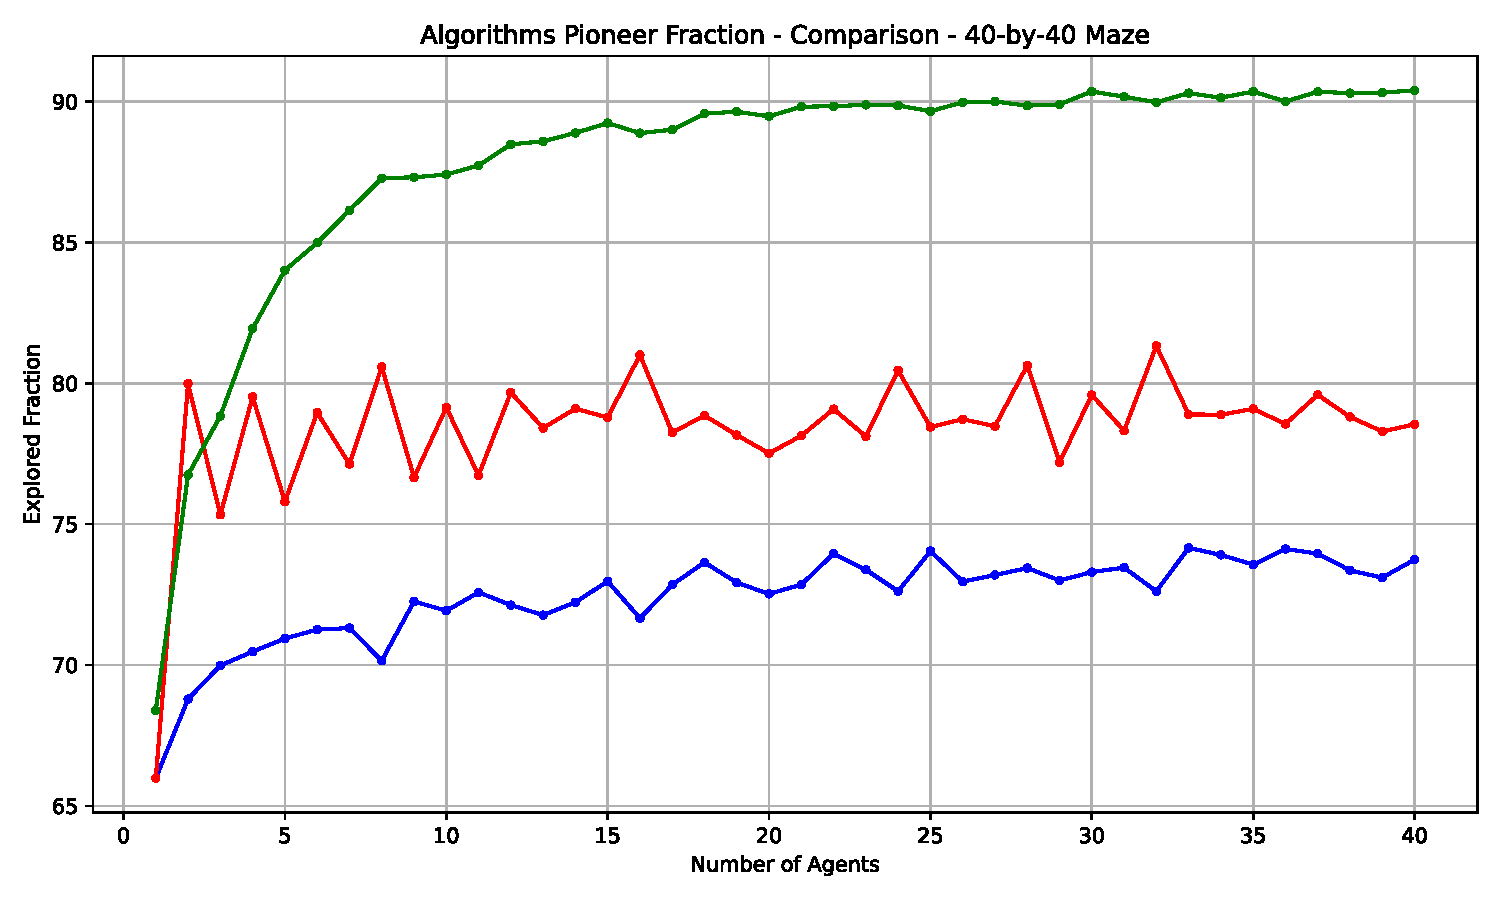
\includegraphics[width=0.45\linewidth]{Cap3/no_comm_fraction__40_by_40_maze.pdf} }}
    \caption{Comparison of the explored fraction achieved by our no-communication algorithms and Tarry's algorithm across different sizes of perfect mazes. The subfigures illustrate how coverage efficiency scales with maze size.}
    \label{fig_no_comm_fraction_all_sizes_maze}
\end{figure}

As this dataset was also used by Rodrigues (2024), and the results shown in Figures \ref{fig_no_comm_steps_all_sizes_maze} and \ref{fig_no_comm_fraction_all_sizes_maze} match his, they confirm the correctness of our new implementation.

The results show that adding more agents helps the pioneer find the goal cell faster, as the average number of steps taken decreases with more agents. This trend eventually levels off at a certain point when there are many agents. The explored fraction behaves similarly, with more agents spreading out quickly and covering more of the maze, though it also stabilizes after a certain number of agents. This outcome is expected, as more agents lead to quicker exploration and better coverage.

In addition to the expected results, the Backward Interval Filling algorithm shows a strange pattern when the number of agents is a power of two, starting from the 20x20 maze size. This matches earlier findings in \cite{Arthur2023}, but it hasn't been fully explored in previous studies. While we recognize the theory suggested by \citen{Arthur2023}, we did not investigate this behavior in detail in our research.

Building on these findings, we compared the performance of our no-communication algorithms with Tarry's algorithm. As expected, both Tarry's algorithm and the Backward Interval Filling variant perform better than the basic version of our algorithm. However, the level of improvement depends on the maze size. In larger mazes, Tarry's algorithm shows a bigger advantage. We conjecture that in smaller mazes, it's possible to quickly find the optimal solution by simply adding more agents. But in larger mazes, communication is crucial for avoiding repeated steps, which we assume significantly enhances Tarry's performance.

\subsection{Random Tree Results} 
\label{subsection_no_comm_random_tree_results}

The results for the random trees of sizes 100, 500, 1000 and 1500 nodes are presented in Figure \ref{fig_no_comm_steps_all_sizes_tree}. These sizes were chosen because they effectively represent the trends observed for the metrics without needing to include every possible size. Figure \ref{fig_no_comm_steps_all_sizes_tree} shows the steps taken by the pioneer, while the Figure \ref{fig_no_comm_fraction_all_sizes_tree} shows the explored fraction.

\begin{figure}[H]
    \centering
    \qquad
    \qquad
    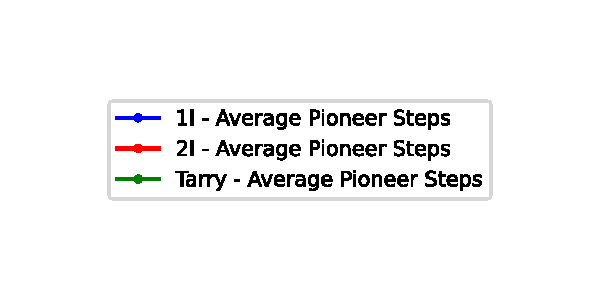
\includegraphics[width=0.5\textwidth]{Cap3/no_comm_steps_legend.pdf}
    \newline
    \subfloat[\centering 100-node Tree]
    {{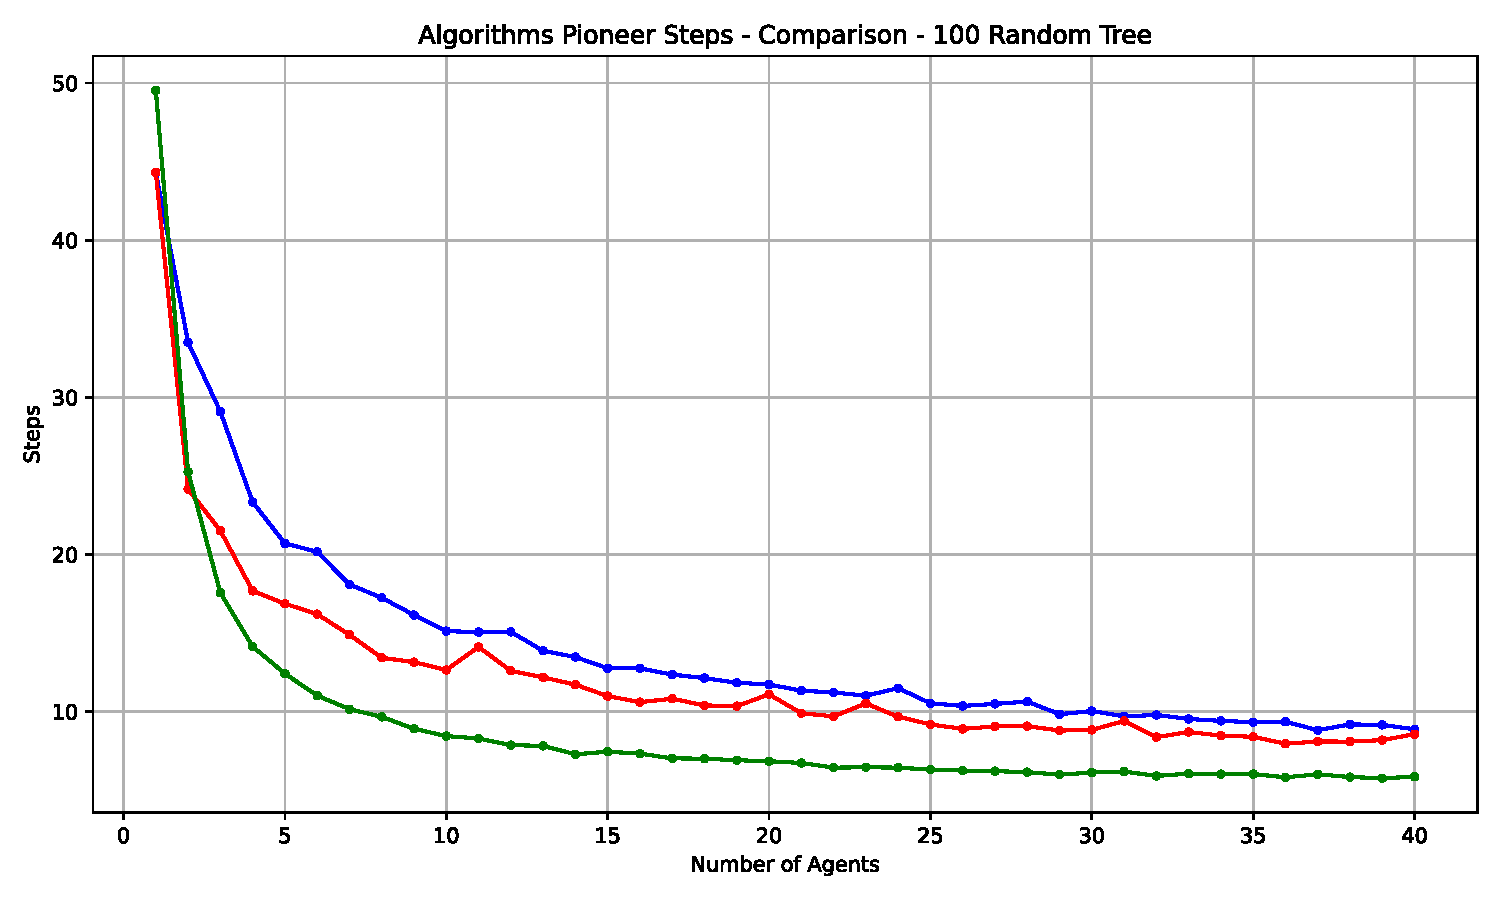
\includegraphics[width=0.45\linewidth]{Cap3/no_comm_steps__100_tree.pdf} }}
    \qquad
    \subfloat[\centering 500-node Tree]
    {{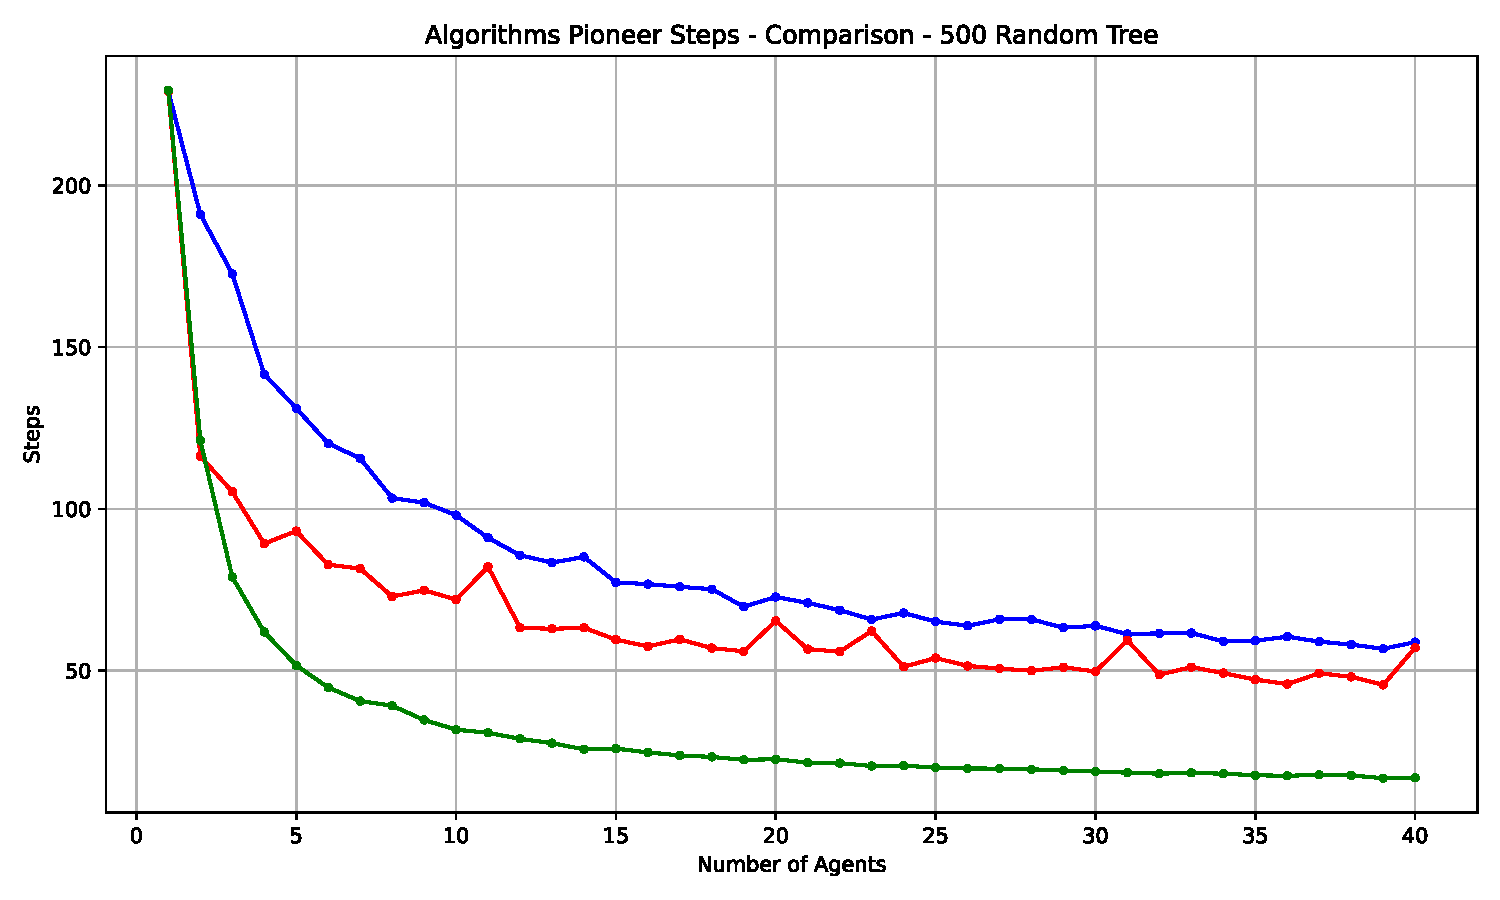
\includegraphics[width=0.45\linewidth]{Cap3/no_comm_steps__500_tree.pdf} }}
    \newline
    \subfloat[\centering 1000-node Tree]
    {{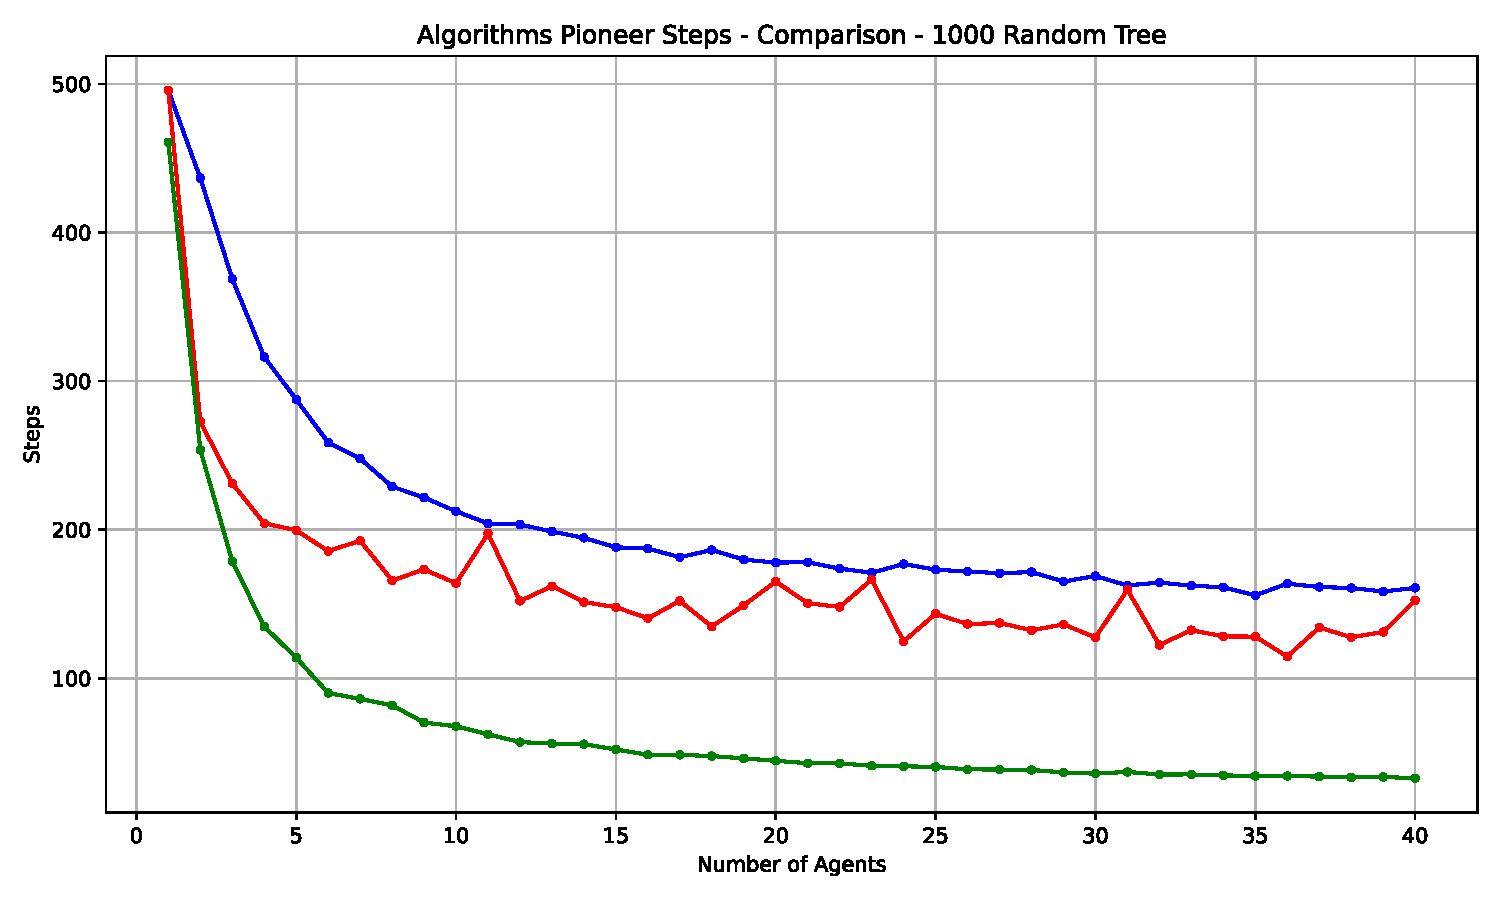
\includegraphics[width=0.45\linewidth]{Cap3/no_comm_steps__1000_tree.pdf} }}
    \qquad
    \subfloat[\centering 1500-node Tree]
    {{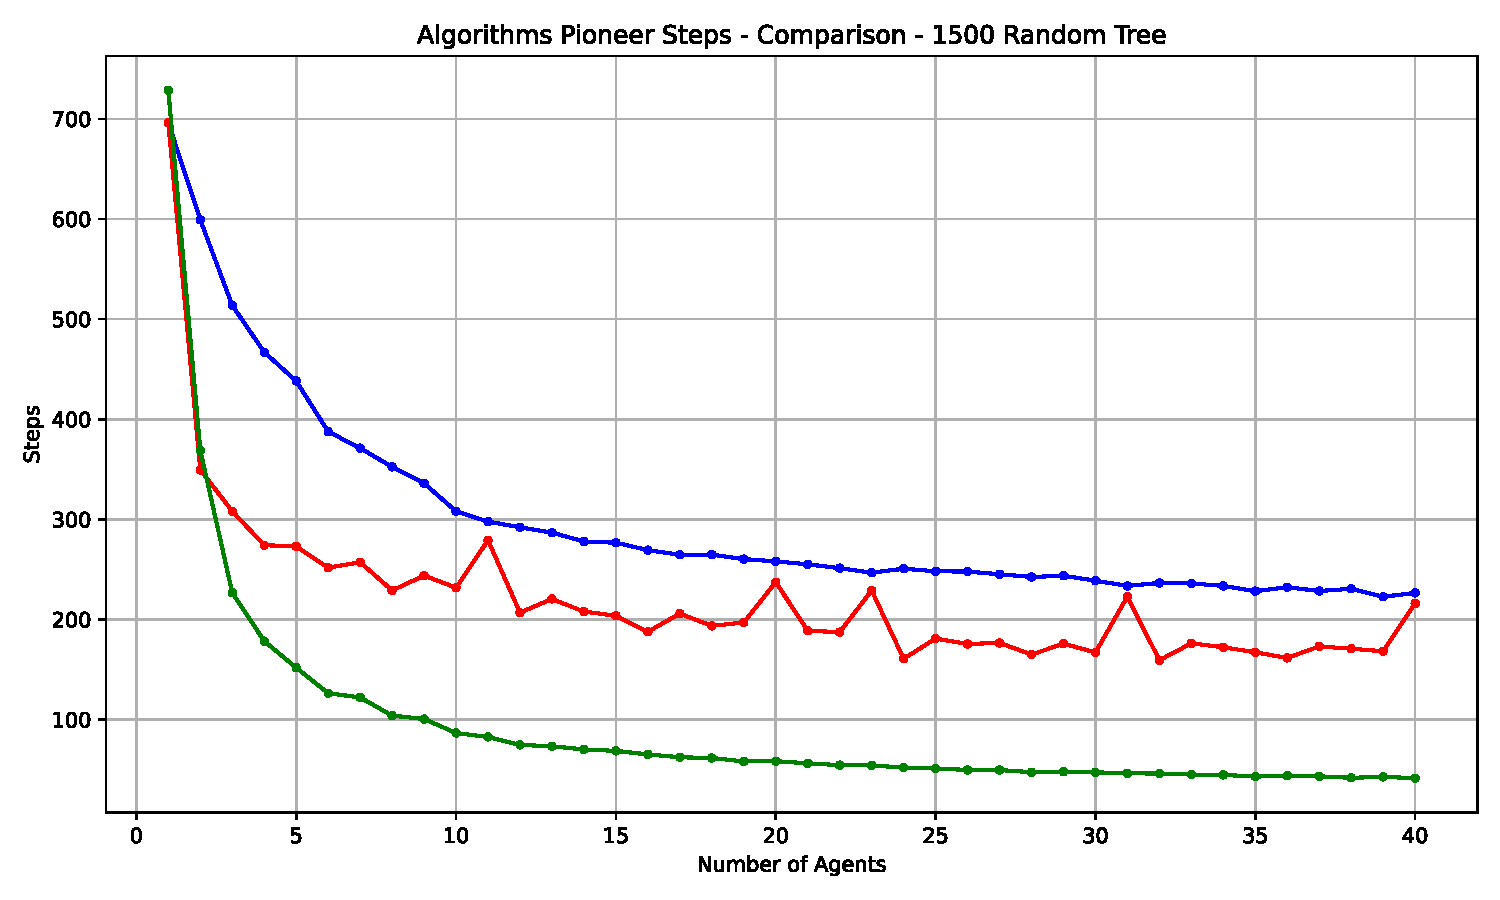
\includegraphics[width=0.45\linewidth]{Cap3/no_comm_steps__1500_tree.pdf} }}
    \caption{Comparison of the average steps taken by the pioneer across different no-communication algorithms and Tarry's algorithm for various sizes of random trees. The subfigures illustrate how algorithm performance varies with tree sizes.}
    \label{fig_no_comm_steps_all_sizes_tree}
\end{figure}

\begin{figure}[H]
    \centering
    \qquad
    \qquad
    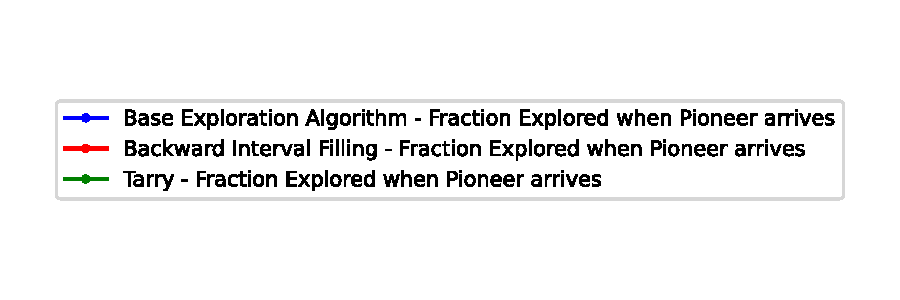
\includegraphics[width=0.5\textwidth]{Cap3/no_comm_fraction_legend.pdf}
    \newline
    \subfloat[\centering 100-node Tree]
    {{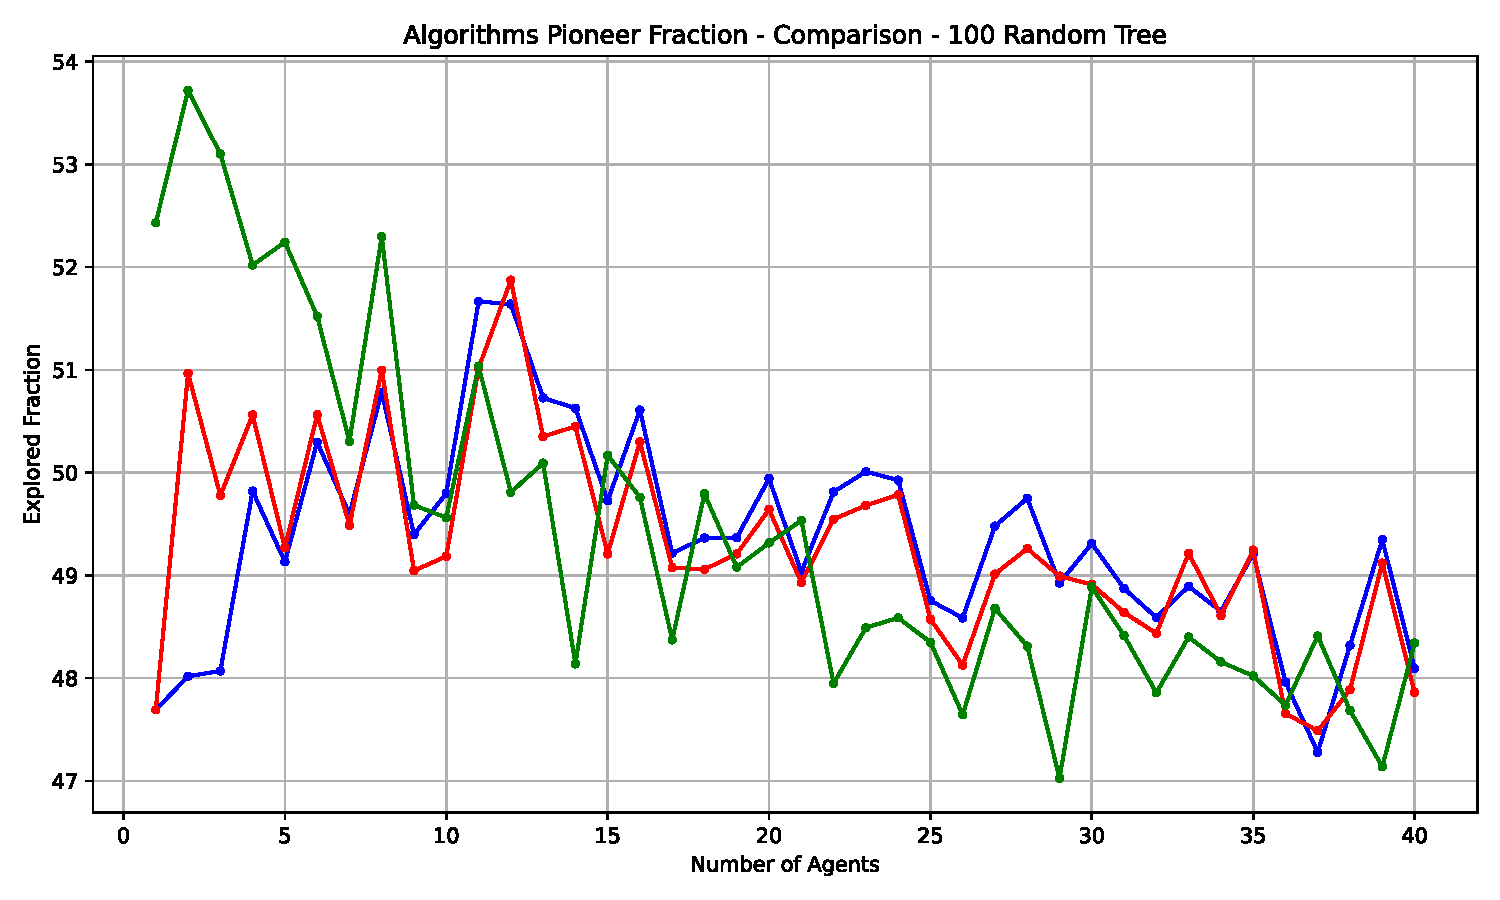
\includegraphics[width=0.45\linewidth]{Cap3/no_comm_fraction__100_tree.pdf} }}
    \qquad
    \subfloat[\centering 500-node Tree]
    {{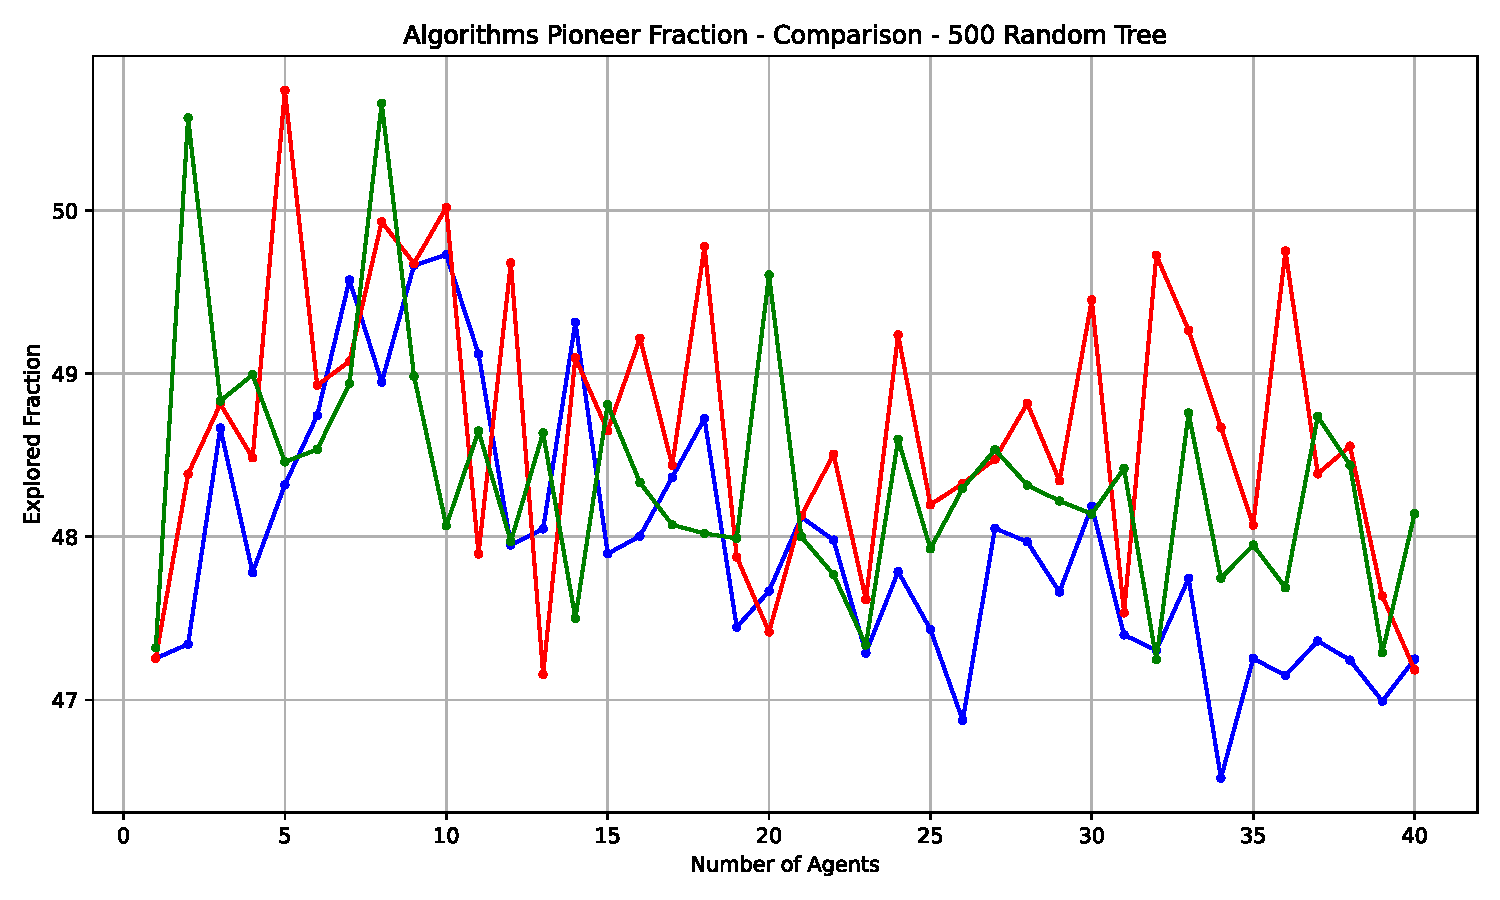
\includegraphics[width=0.45\linewidth]{Cap3/no_comm_fraction__500_tree.pdf} }}
    \newline
    \subfloat[\centering 1000-node Tree]
    {{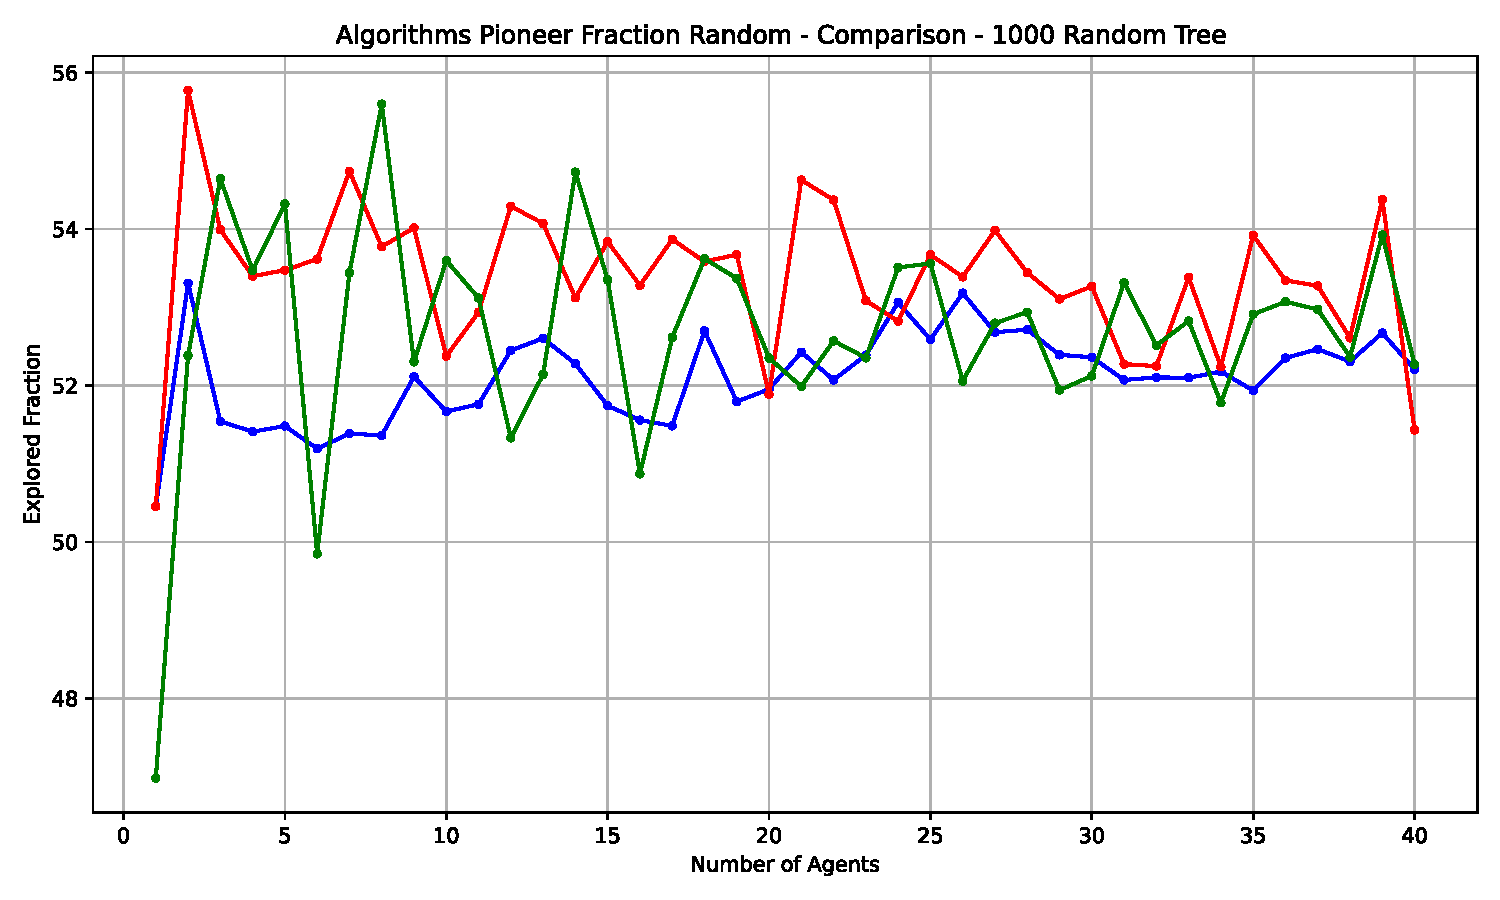
\includegraphics[width=0.45\linewidth]{Cap3/no_comm_fraction__1000_tree.pdf} }}
    \qquad
    \subfloat[\centering 1500-node Tree]
    {{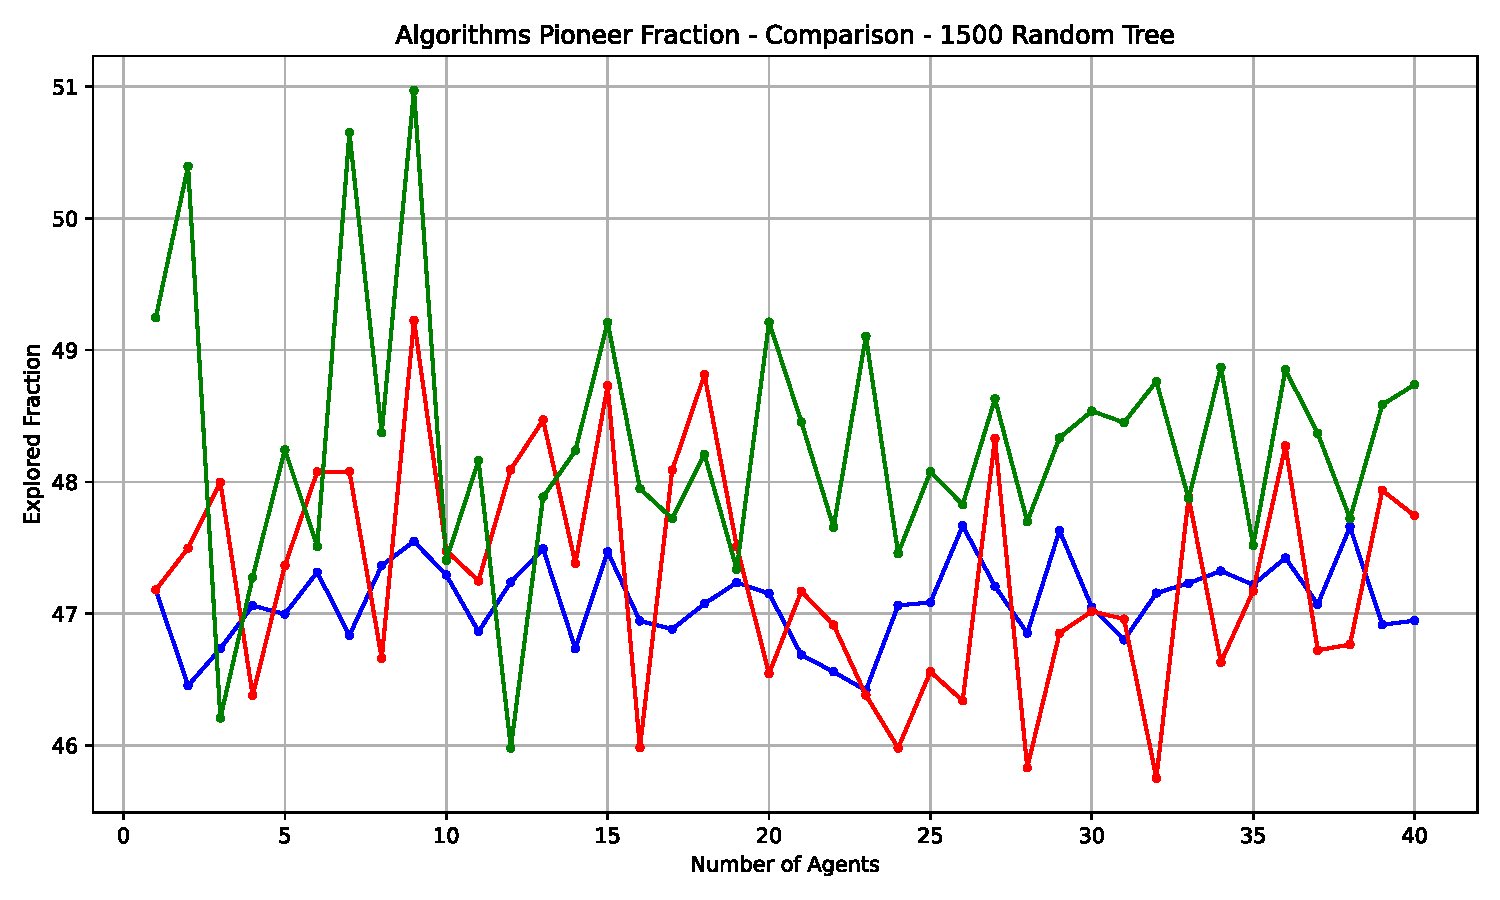
\includegraphics[width=0.45\linewidth]{Cap3/no_comm_fraction__1500_tree.pdf} }}
    \caption{Comparison of the explored fraction achieved by the pioneer across different no-communication algorithms and Tarry's algorithm for various sizes of random trees. The subfigures illustrate how coverage efficiency varies with tree sizes.}
    \label{fig_no_comm_fraction_all_sizes_tree}
\end{figure}

The results for the random trees confirm that the conclusions from Section \ref{subsection_no_comm_maze_results} still apply. Performance improves with more agents, Tarry's algorithm remains the most efficient, and its advantages increase with size.

Even though the trends hold, it's important to note that Tarry outperforms the Back Filling Interval Variation by approximately 39.6\% and our proposed algorithm by 47.3\% in the 40x40 maze. In contrast, in the 1500-node trees, Tarry shows a substantial improvement, being about 81.7\% better than our proposed algorithm and 80.8\% better than the Back Filling Interval Variation. This demonstrates the significant impact of dataset characteristics on the relative performance of our no-communication algorithms.

Referring to Figure \ref{fig_no_comm_fraction_all_sizes_tree}, the results differ from expectations, as the plots are noisy and don't show a clear pattern where Tarry's algorithm consistently explores a larger fraction. Previously, the explored fraction increased with the number of agents, but that trend isn't evident here, as all the algorithms are around the same values with little difference regardless of the number of agents.

This difference arises from the dataset characteristics. In deep trees like Perfect Mazes, agents must explore down to the leaf nodes to find the goal, setting a lower limit on the number of steps. In shallower trees like Random Trees, agents can quickly reach leaf nodes, potentially finding the goal earlier regardless of agent count.

As a result, some instances show a very small explored fraction, while others have a higher one, leading to noisy averages. For example, considering Tarry's with 1500 nodes and 20 agents, the explored fraction averaged 49.21\% with a standard deviation of 30.07\%, highlighting this variability. This large spread means this metric is not very relevant for this kind of dataset. On the other hand, zero-communication algorithms do not incur on any loss with respect to this metric.

\begin{figure}[H]
    \centering 
    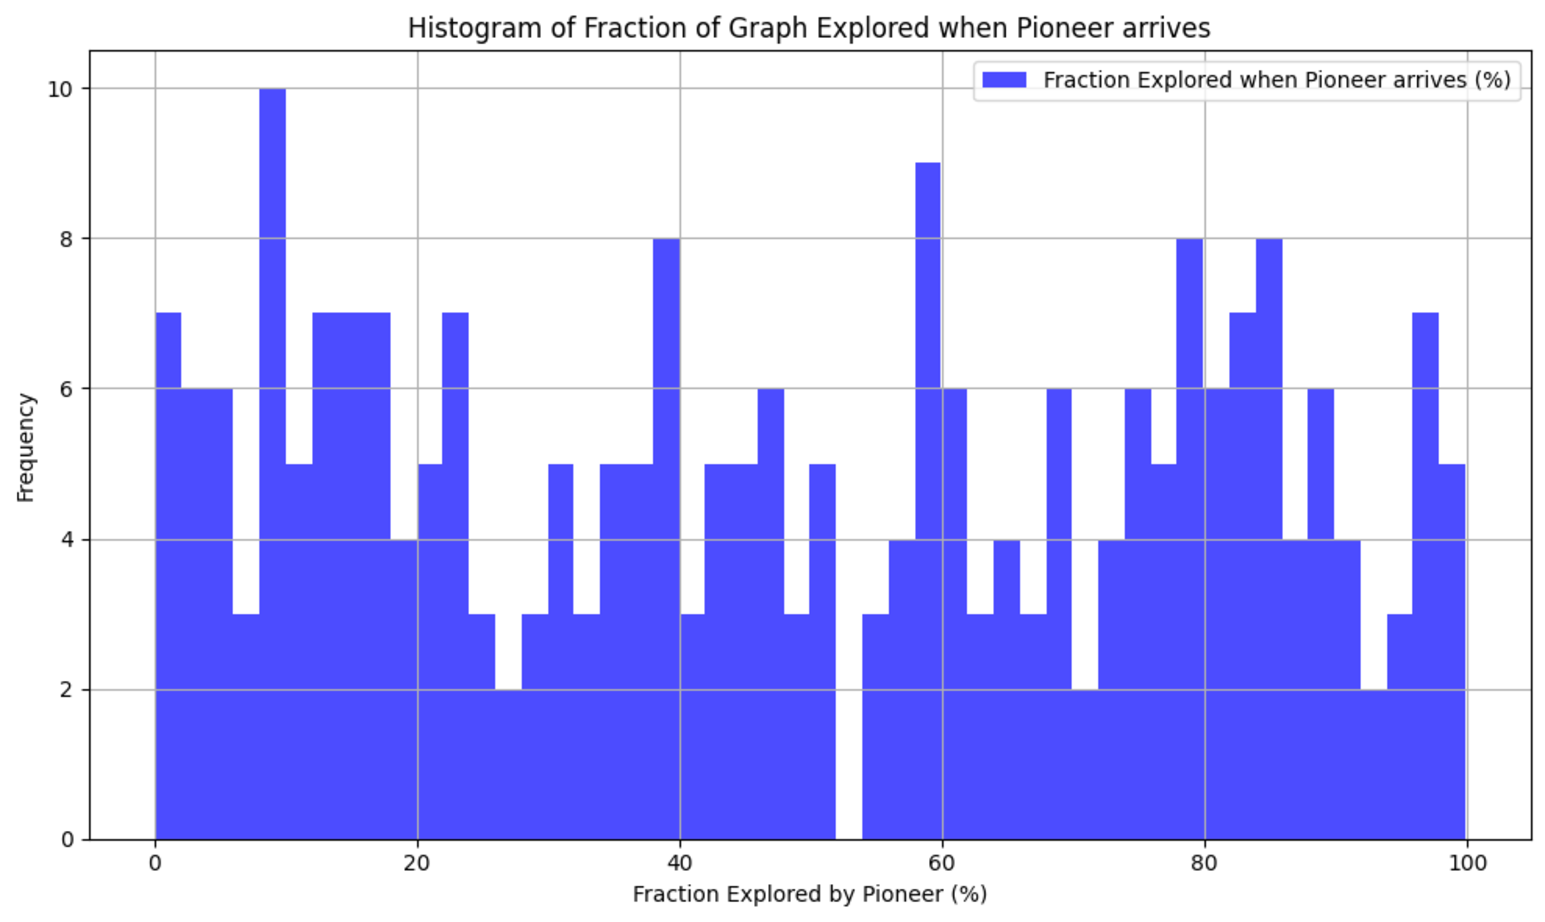
\includegraphics[width=0.7\textwidth]{Cap3/no_comm_fraction_histogram_tree.pdf} 
    \caption{Histogram of explored fractions for random trees with 1500 nodes and 20 agents using Tarry's Algorithm.} 
    \label{fig_no_comm_fraction_histogram_tree}
\end{figure}

As expected, Figure \ref{fig_no_comm_fraction_histogram_tree} shows a fairly uniform distribution in the explored fractions, reflecting the characteristics of the random trees.

\subsection{Barabási-Albert Results} 
\label{subsection_no_comm_barabasi_albert_results}

The results for the Barabási-Albert graphs with 100, 250, 500, and 1000 nodes are shown in Figures \ref{fig_no_comm_steps_all_sizes_barabasi} and \ref{fig_no_comm_fraction_all_sizes_barabasi}. These sizes were selected to capture the overall trends in exploration efficiency while accounting for computational constraints on larger Barabási-Albert graphs. Notably, for the 1000-node graph, the maximum number of agents was limited to 30 instead of the standard 40 due to performance considerations. Figure \ref{fig_no_comm_steps_all_sizes_barabasi} illustrates the average steps taken by the pioneer, while Figure \ref{fig_no_comm_fraction_all_sizes_barabasi} displays the explored fraction achieved.

\begin{figure}[H]
    \centering
    \qquad
    \qquad
    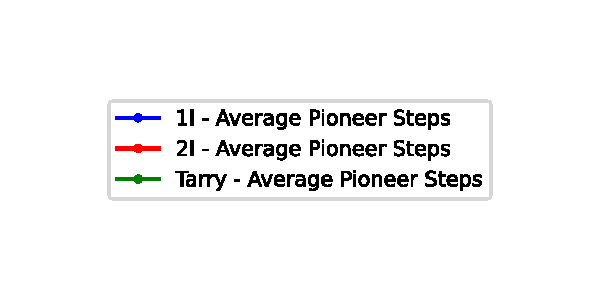
\includegraphics[width=0.5\textwidth]{Cap3/no_comm_steps_legend.pdf}
    \newline
    \subfloat[\centering 100-node Barabási-Albert]
    {{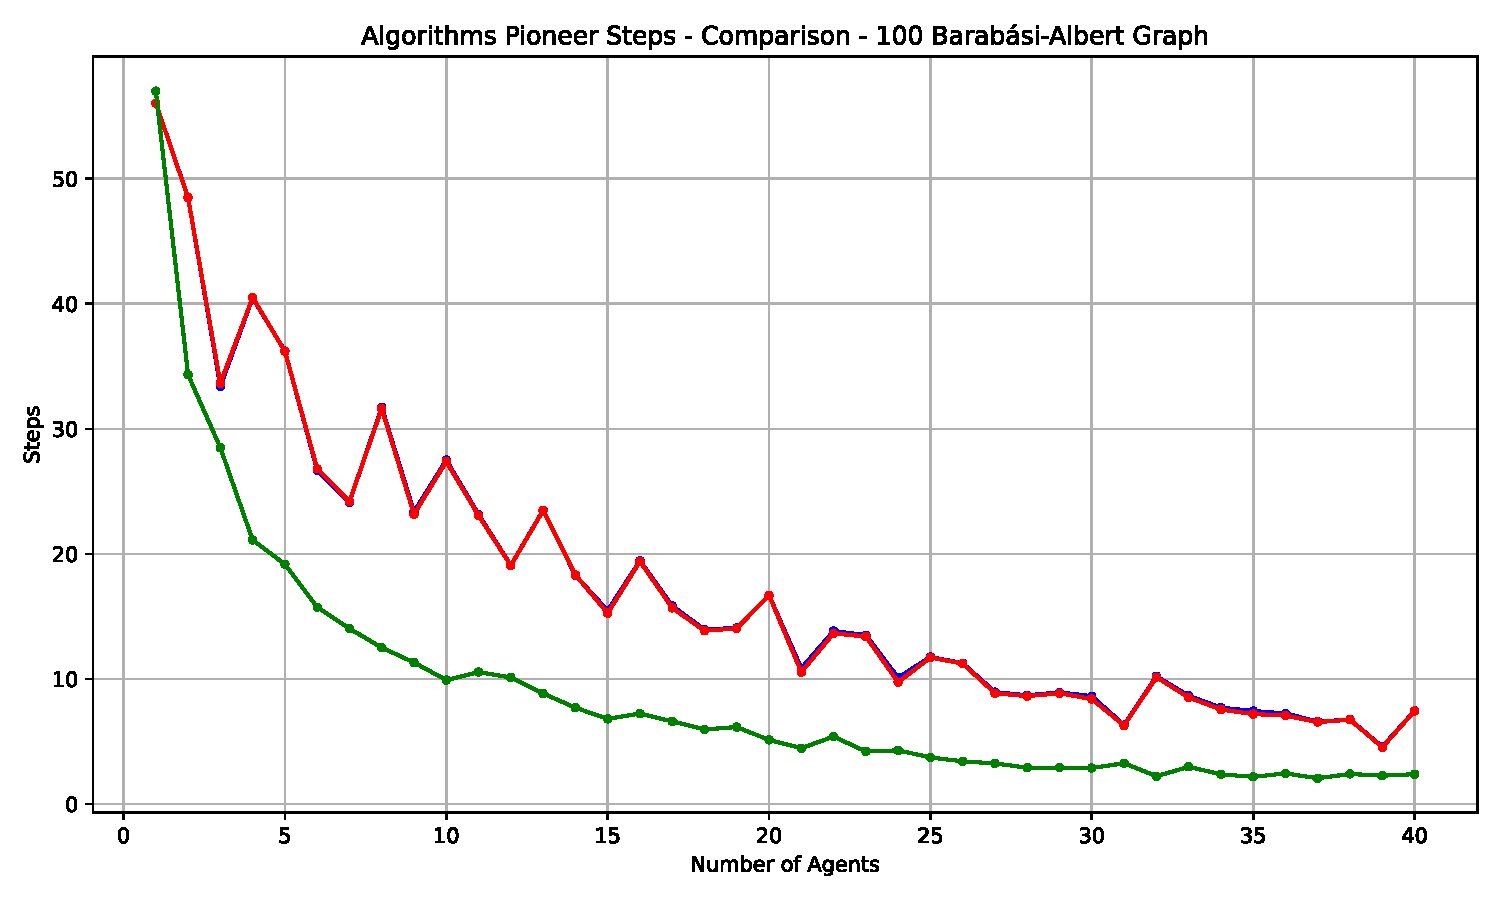
\includegraphics[width=0.45\linewidth]{Cap3/no_comm_steps__100_barabasi.pdf} }}
    \qquad
    \subfloat[\centering 250-node Barabási-Albert]
    {{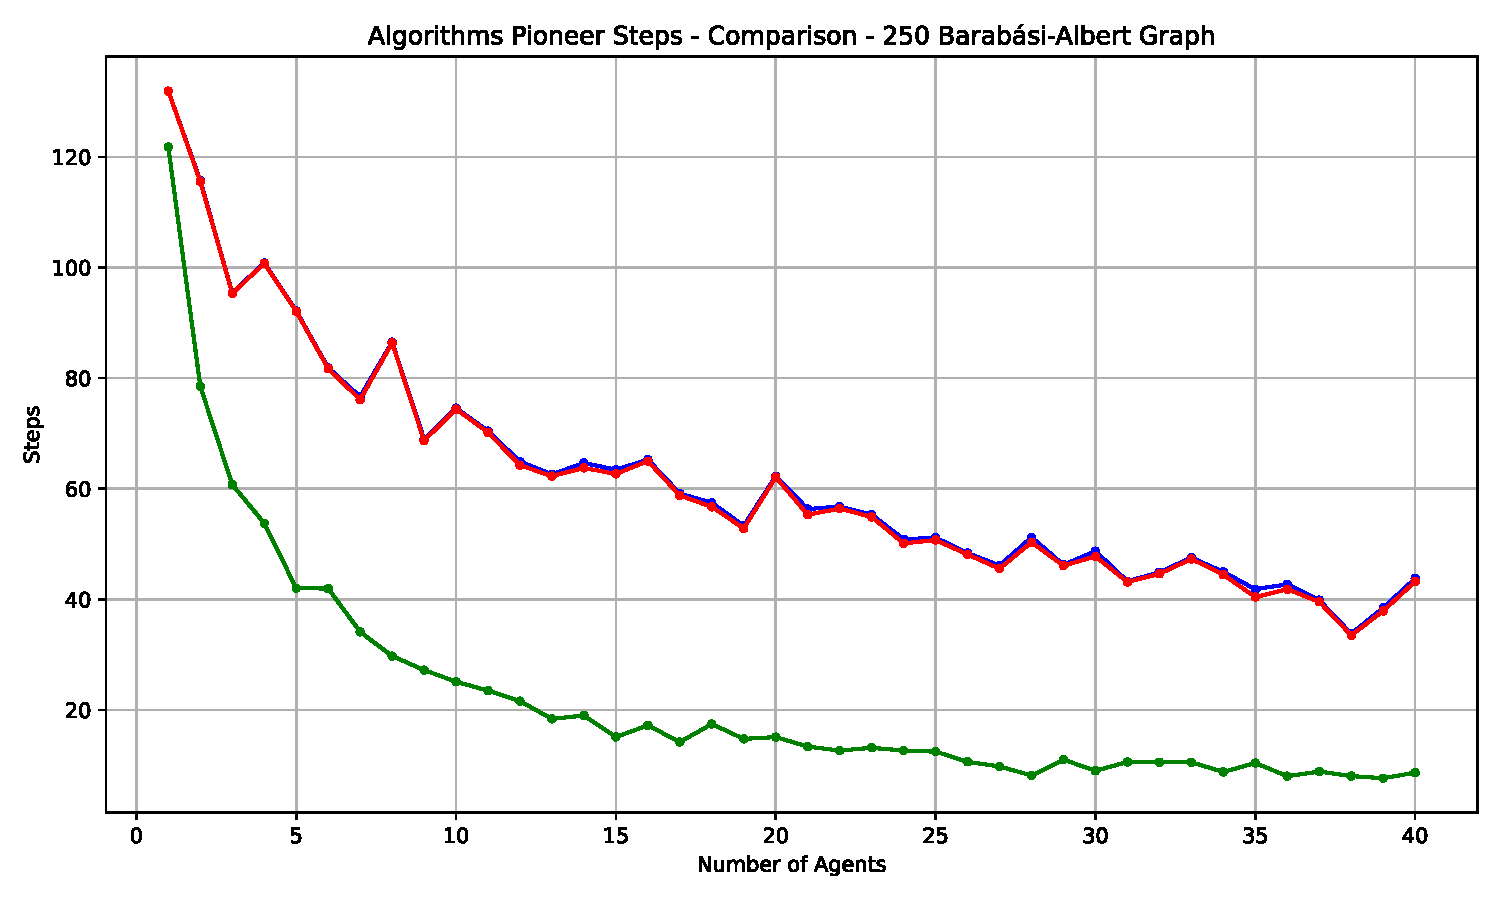
\includegraphics[width=0.45\linewidth]{Cap3/no_comm_steps__250_barabasi.pdf} }}
    \newline
    \subfloat[\centering 500-node Barabási-Albert]
    {{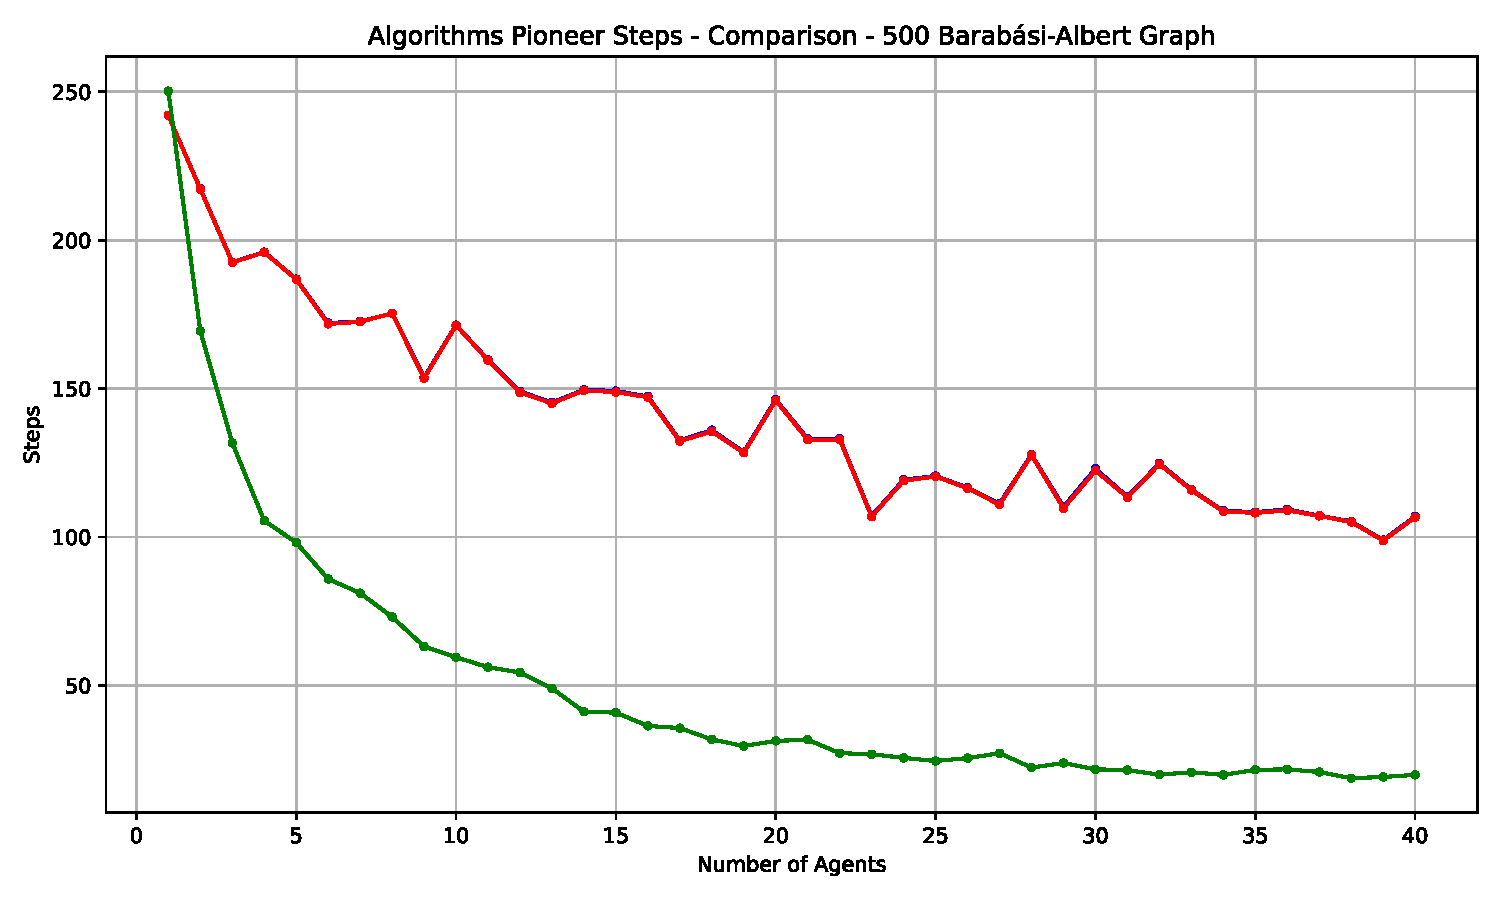
\includegraphics[width=0.45\linewidth]{Cap3/no_comm_steps__500_barabasi.pdf} }}
    \qquad
    \subfloat[\centering 1000-node Barabási-Albert]
    {{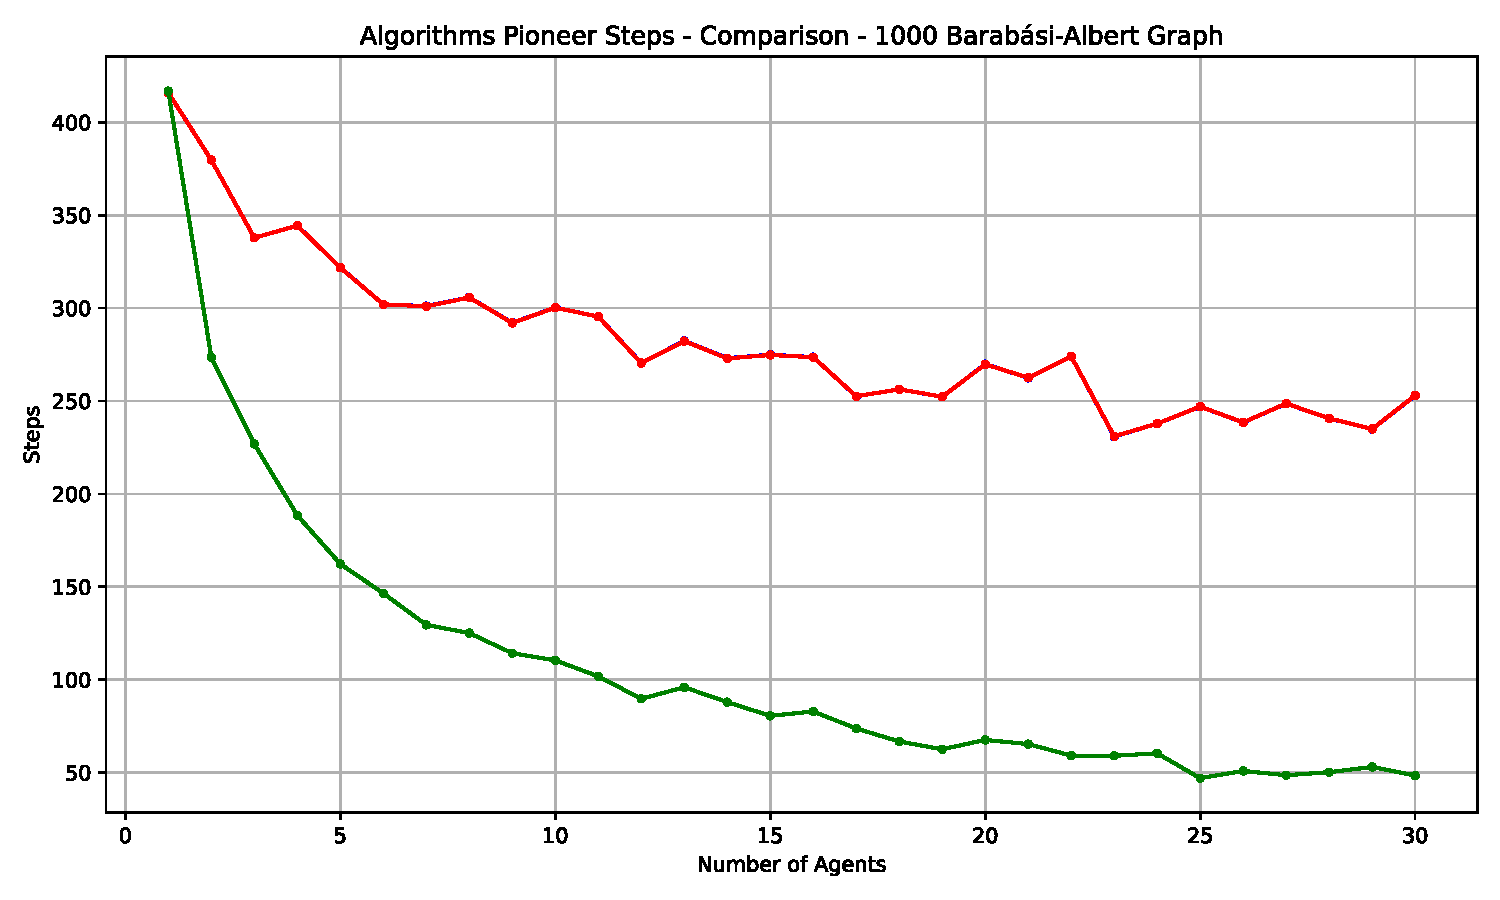
\includegraphics[width=0.45\linewidth]{Cap3/no_comm_steps__1000_barabasi.pdf} }}
    \caption{Comparison of the average steps taken by the pioneer across different no-communication algorithms and Tarry's algorithm for various sizes of Barabási-Albert graphs. The subfigures illustrate how algorithm performance varies with graph sizes.}
    \label{fig_no_comm_steps_all_sizes_barabasi}
\end{figure}

\begin{figure}[H]
    \centering
    \qquad
    \qquad
    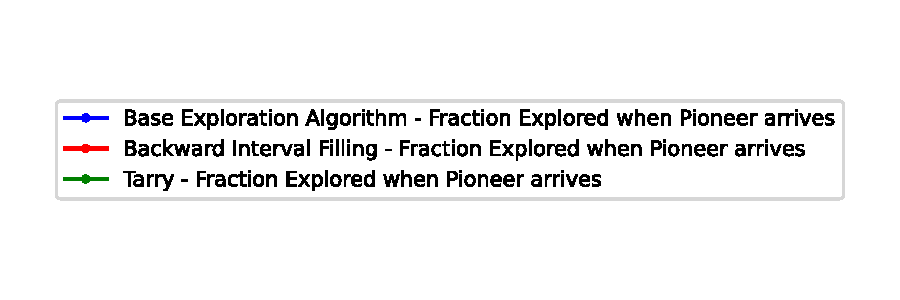
\includegraphics[width=0.5\textwidth]{Cap3/no_comm_fraction_legend.pdf}
    \newline
    \subfloat[\centering 100-node Barabási-Albert]
    {{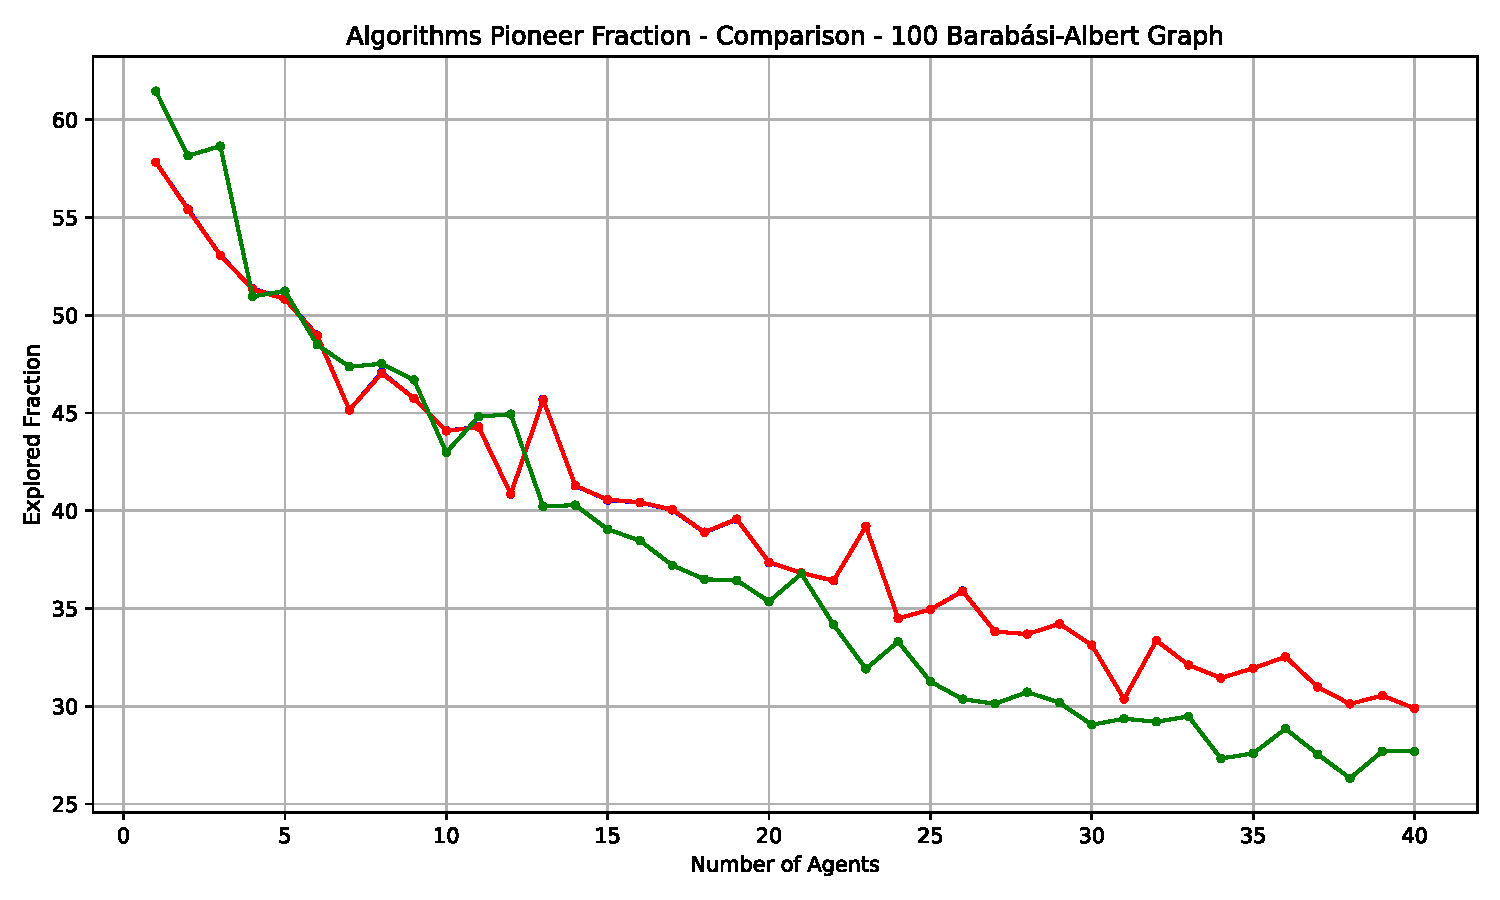
\includegraphics[width=0.45\linewidth]{Cap3/no_comm_fraction__100_barabasi.pdf} }}
    \qquad
    \subfloat[\centering 250-node Barabási-Albert]
    {{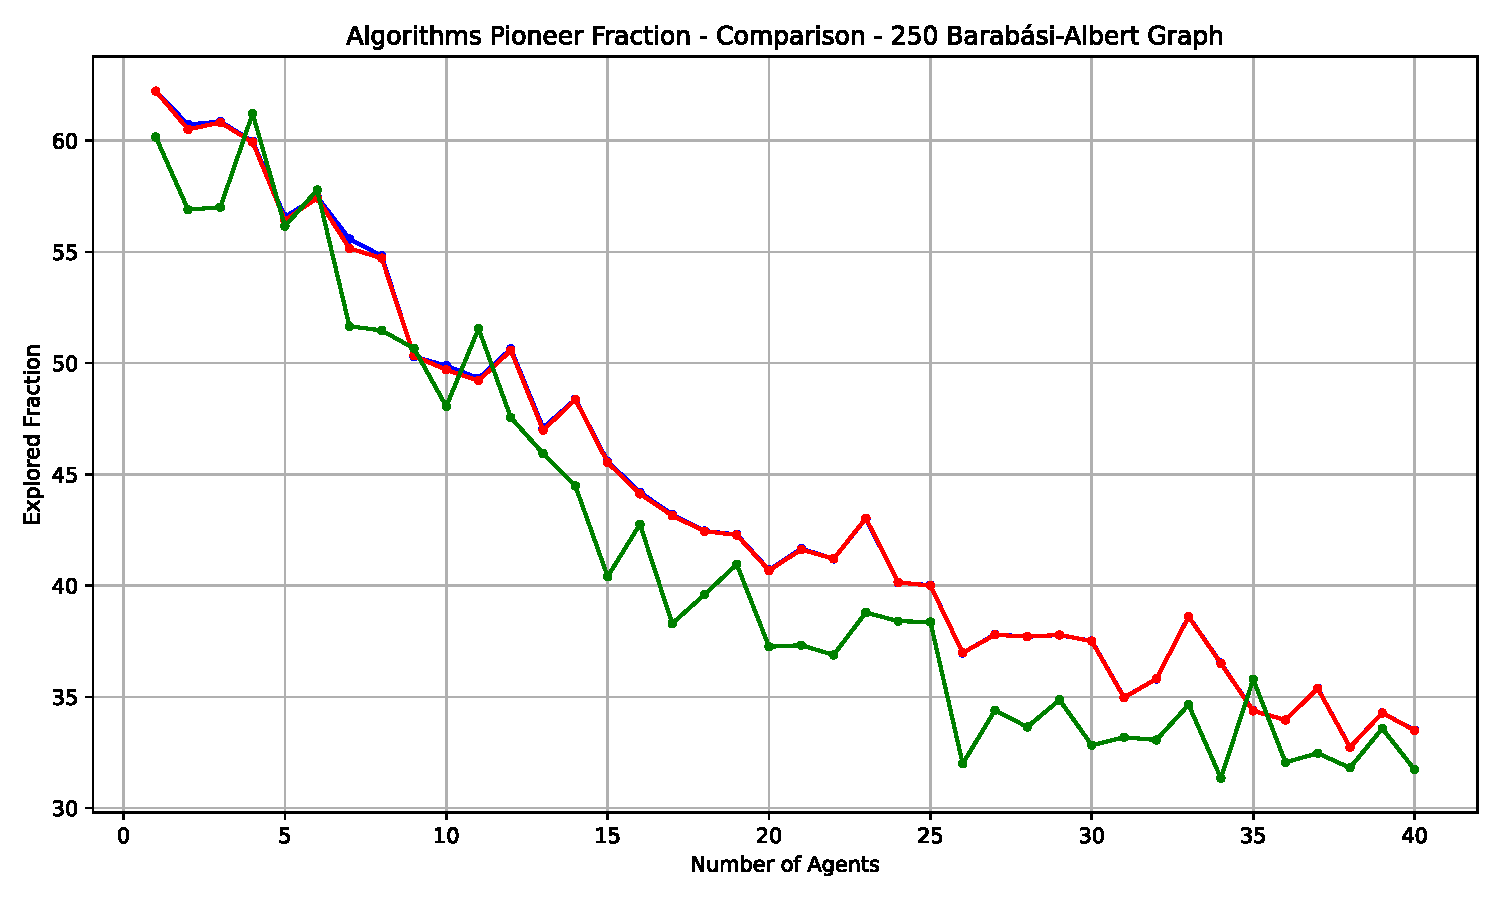
\includegraphics[width=0.45\linewidth]{Cap3/no_comm_fraction__250_barabasi.pdf} }}
    \newline
    \subfloat[\centering 500-node Barabási-Albert]
    {{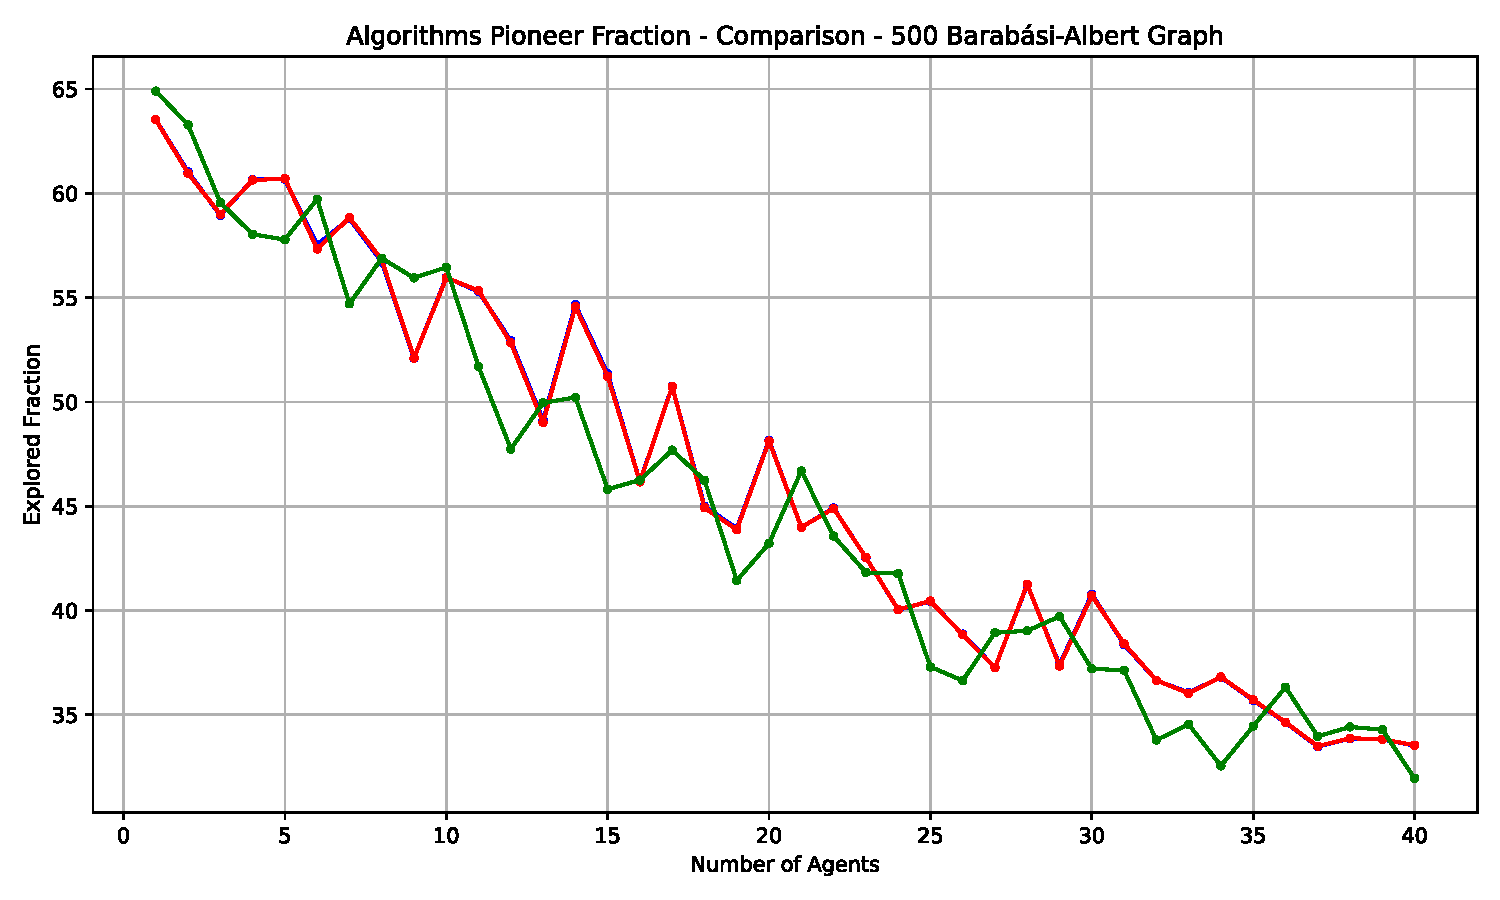
\includegraphics[width=0.45\linewidth]{Cap3/no_comm_fraction__500_barabasi.pdf} }}
    \qquad
    \subfloat[\centering 1000-node Barabási-Albert]
    {{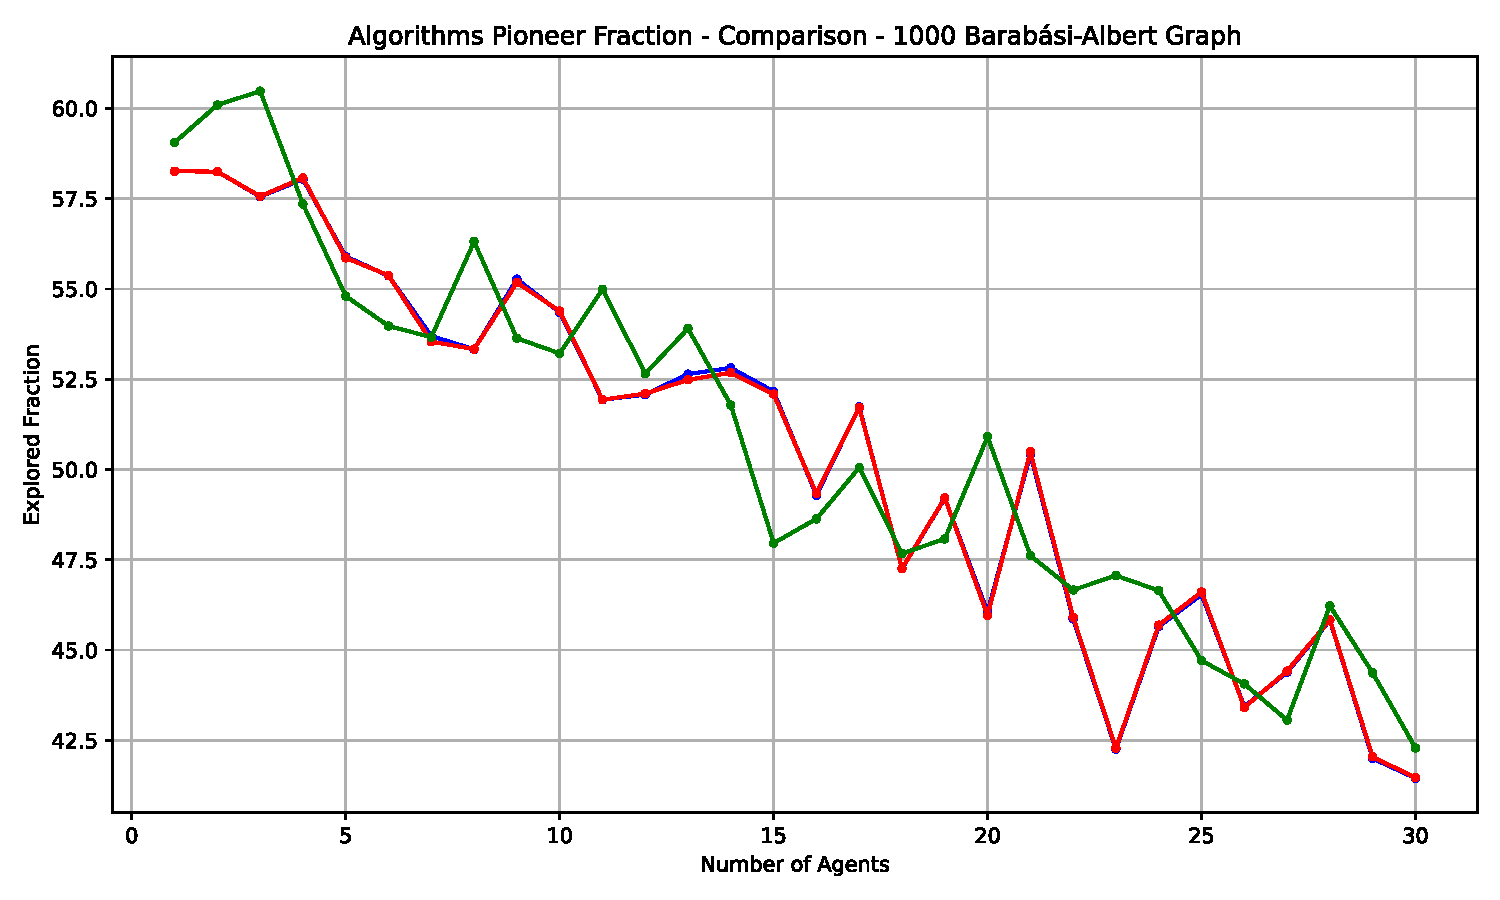
\includegraphics[width=0.45\linewidth]{Cap3/no_comm_fraction__1000_barabasi.pdf} }}
    \caption{Comparison of the explored fraction achieved by the pioneer across different no-communication algorithms and Tarry's algorithm for various sizes of Barabási-Albert graphs. The subfigures illustrate how coverage efficiency varies with graph sizes.}
    \label{fig_no_comm_fraction_all_sizes_barabasi}
\end{figure}

As expected, performance improves with more agents, and Tarry's algorithm remains the most effective approach. However, for this dataset, the Backward Interval Filling algorithm shows no improvement over the basic exploration algorithm. We suspect this is because the Barabási-Albert graphs are highly connected and contain many cycles, leading each agent to form a distinct exploration tree. The same nodes often have significantly different intervals based on the paths taken by each agent. Consequently, each agent completes its initial interval and often reaches the goal before starting a second one.

Unlike the trend observed in Section \ref{subsection_no_comm_maze_results}, the explored fraction decreases with additional agents. This likely occurs because the multiple cycles lead to frequent intersections between agents' exploration trees, adding redundant information. As agents reach the goal quickly, there is less time to explore other parts of the graph.

\subsection{Small-World Results} 
\label{subsection_no_comm_sw_results}

The results for Small-World graphs with 100, 250, 500, and 1000 nodes are shown in Figures \ref{fig_no_comm_steps_all_sizes_sw} and \ref{fig_no_comm_fraction_all_sizes_sw}. These sizes were chosen to capture overall trends in exploration efficiency within computational limits for larger graphs. For the 100-node and 250-node graphs, up to 40 agents were used, while for the 500-node and 1000-node graphs, the maximum was limited to 30 agents due to performance constraints.

\begin{figure}[H]
    \centering
    \qquad
    \qquad
    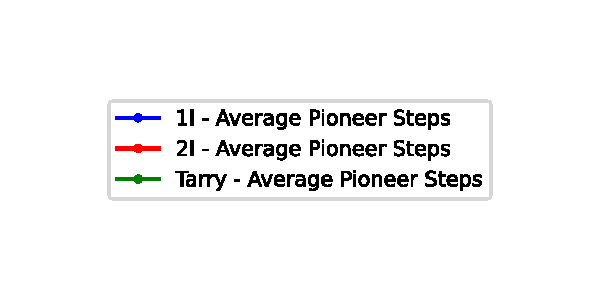
\includegraphics[width=0.5\textwidth]{Cap3/no_comm_steps_legend.pdf}
    \newline
    \subfloat[\centering 100-node Small-World]
    {{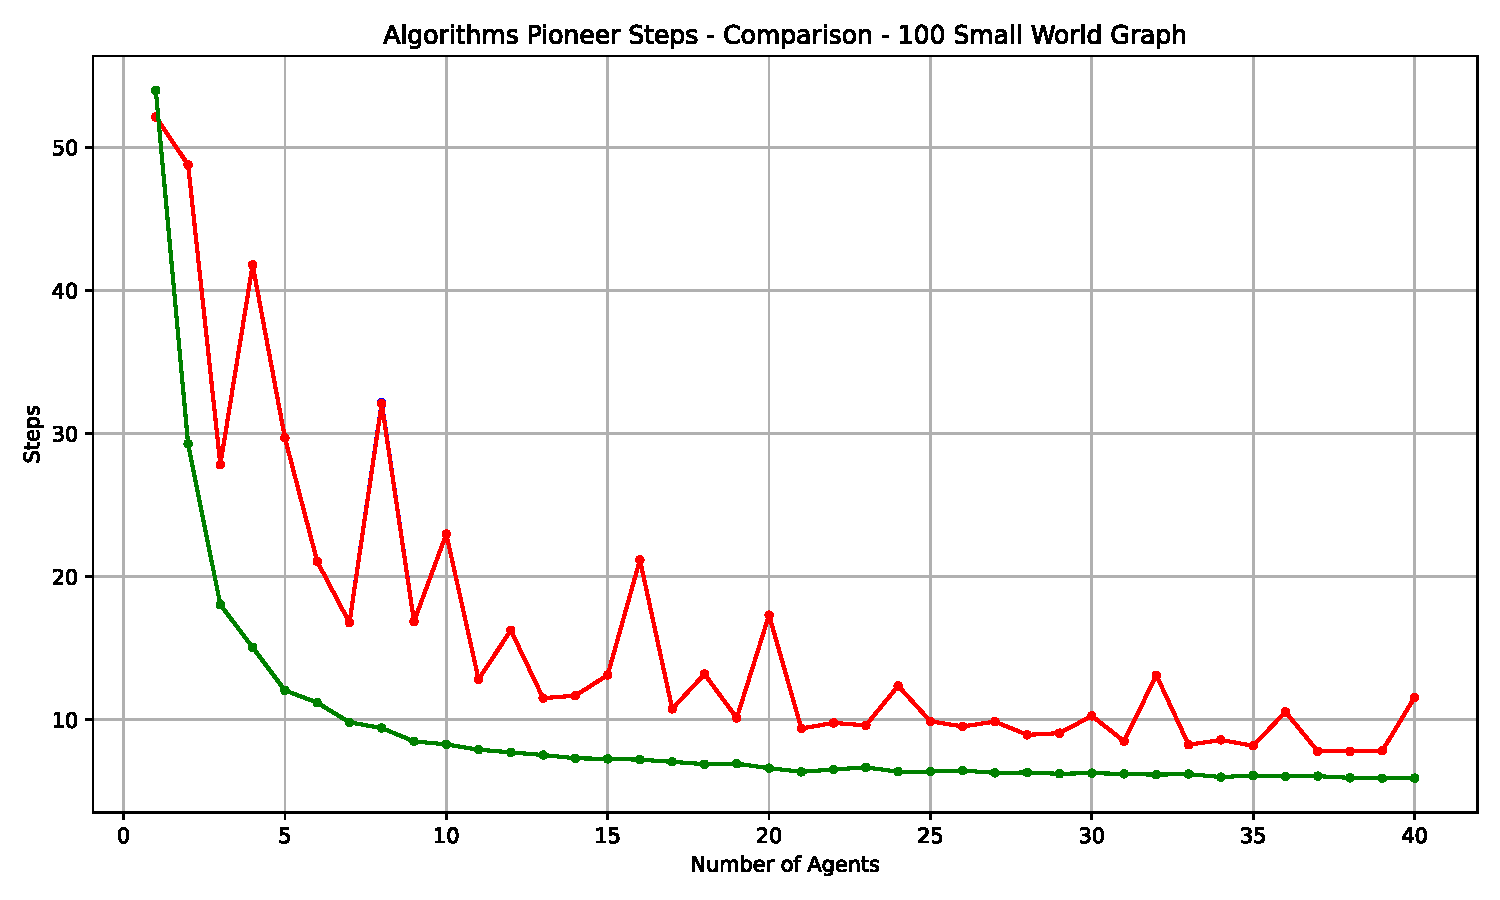
\includegraphics[width=0.45\linewidth]{Cap3/no_comm_steps__100_sw.pdf} }}
    \qquad
    \subfloat[\centering 250-node Small-World]
    {{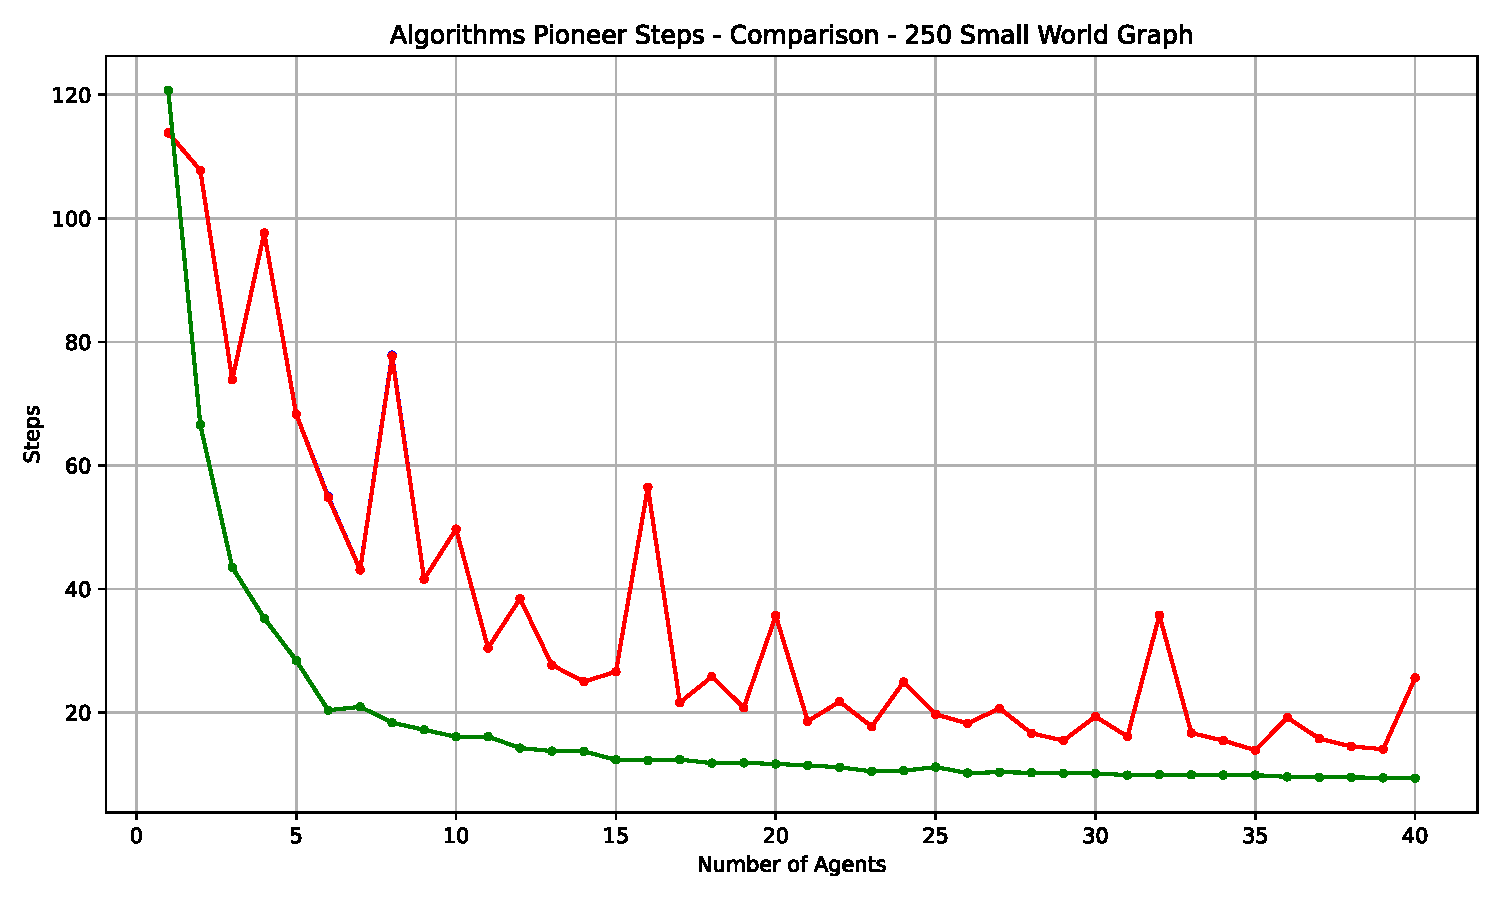
\includegraphics[width=0.45\linewidth]{Cap3/no_comm_steps__250_sw.pdf} }}
    \newline
    \subfloat[\centering 500-node Small-World]
    {{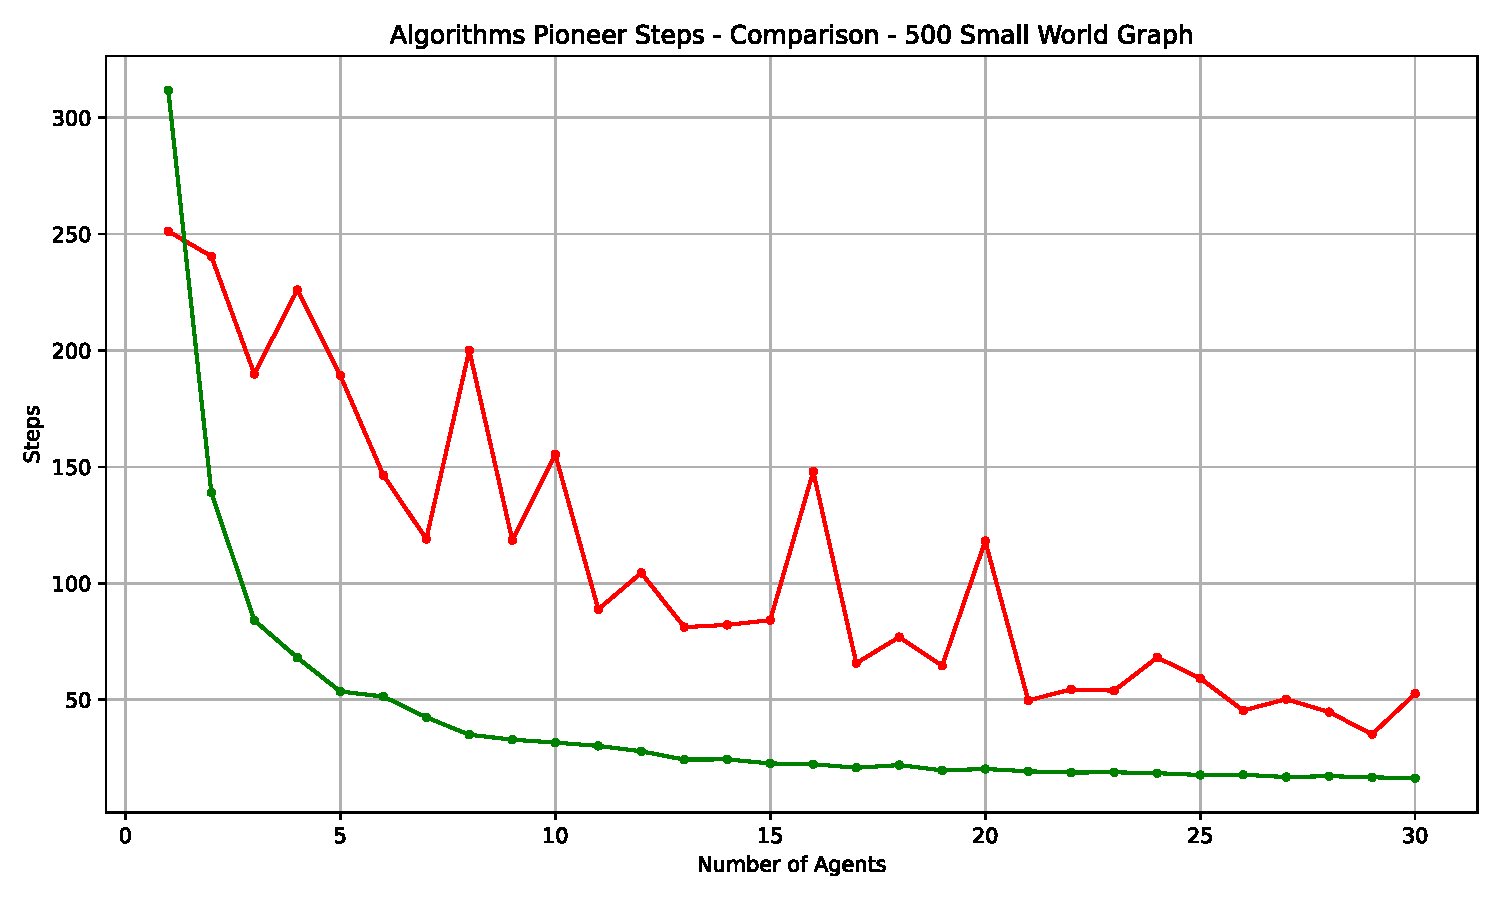
\includegraphics[width=0.45\linewidth]{Cap3/no_comm_steps__500_sw.pdf} }}
    \qquad
    \subfloat[\centering 1000-node Small-World]
    {{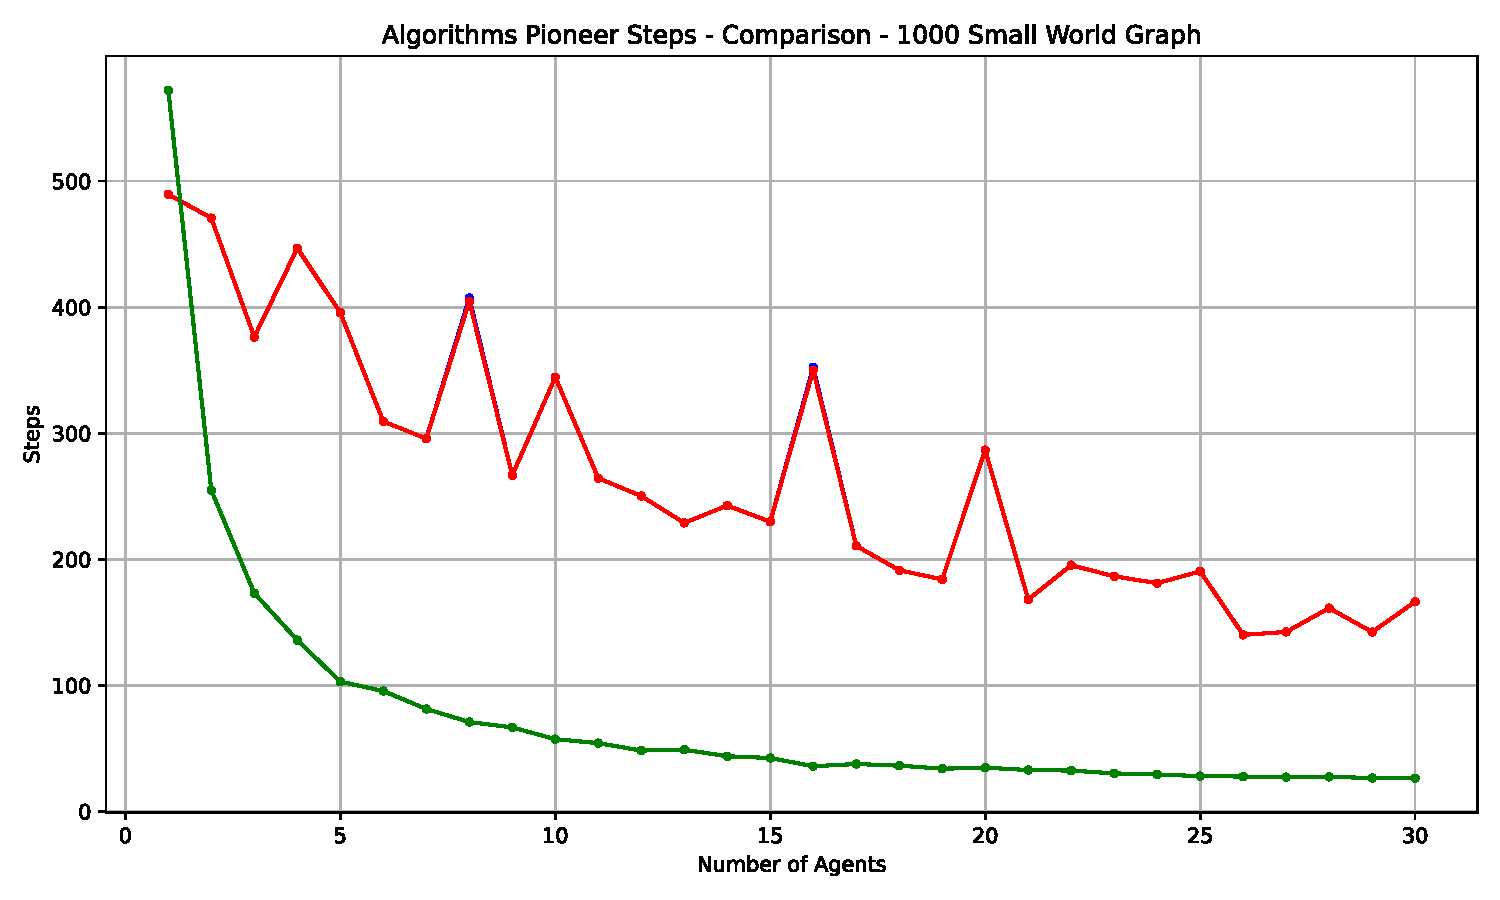
\includegraphics[width=0.45\linewidth]{Cap3/no_comm_steps__1000_sw.pdf} }}
    \caption{Comparison of the average steps taken by the pioneer across different no-communication algorithms and Tarry's algorithm for various sizes of Small-World graphs. The subfigures illustrate how algorithm performance varies with graph sizes.}
    \label{fig_no_comm_steps_all_sizes_sw}
\end{figure}

\begin{figure}[H]
    \centering
    \qquad
    \qquad
    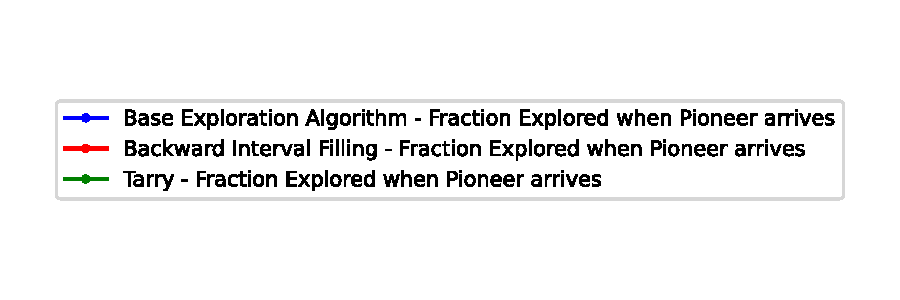
\includegraphics[width=0.5\textwidth]{Cap3/no_comm_fraction_legend.pdf}
    \newline
    \subfloat[\centering 100-node Small-World]
    {{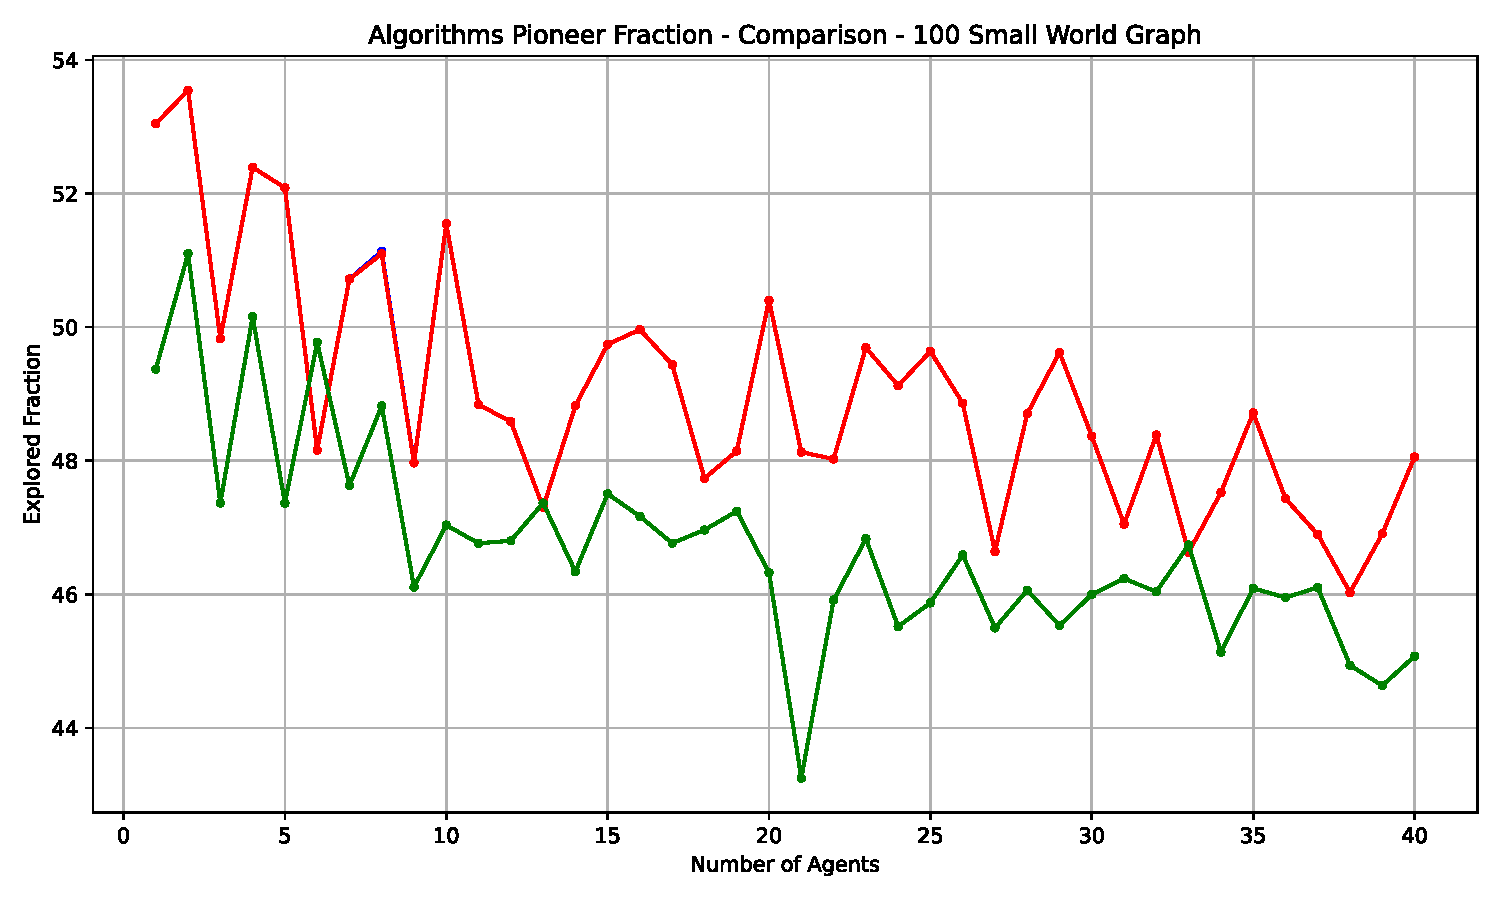
\includegraphics[width=0.45\linewidth]{Cap3/no_comm_fraction__100_sw.pdf} }}
    \qquad
    \subfloat[\centering 250-node Small-World]
    {{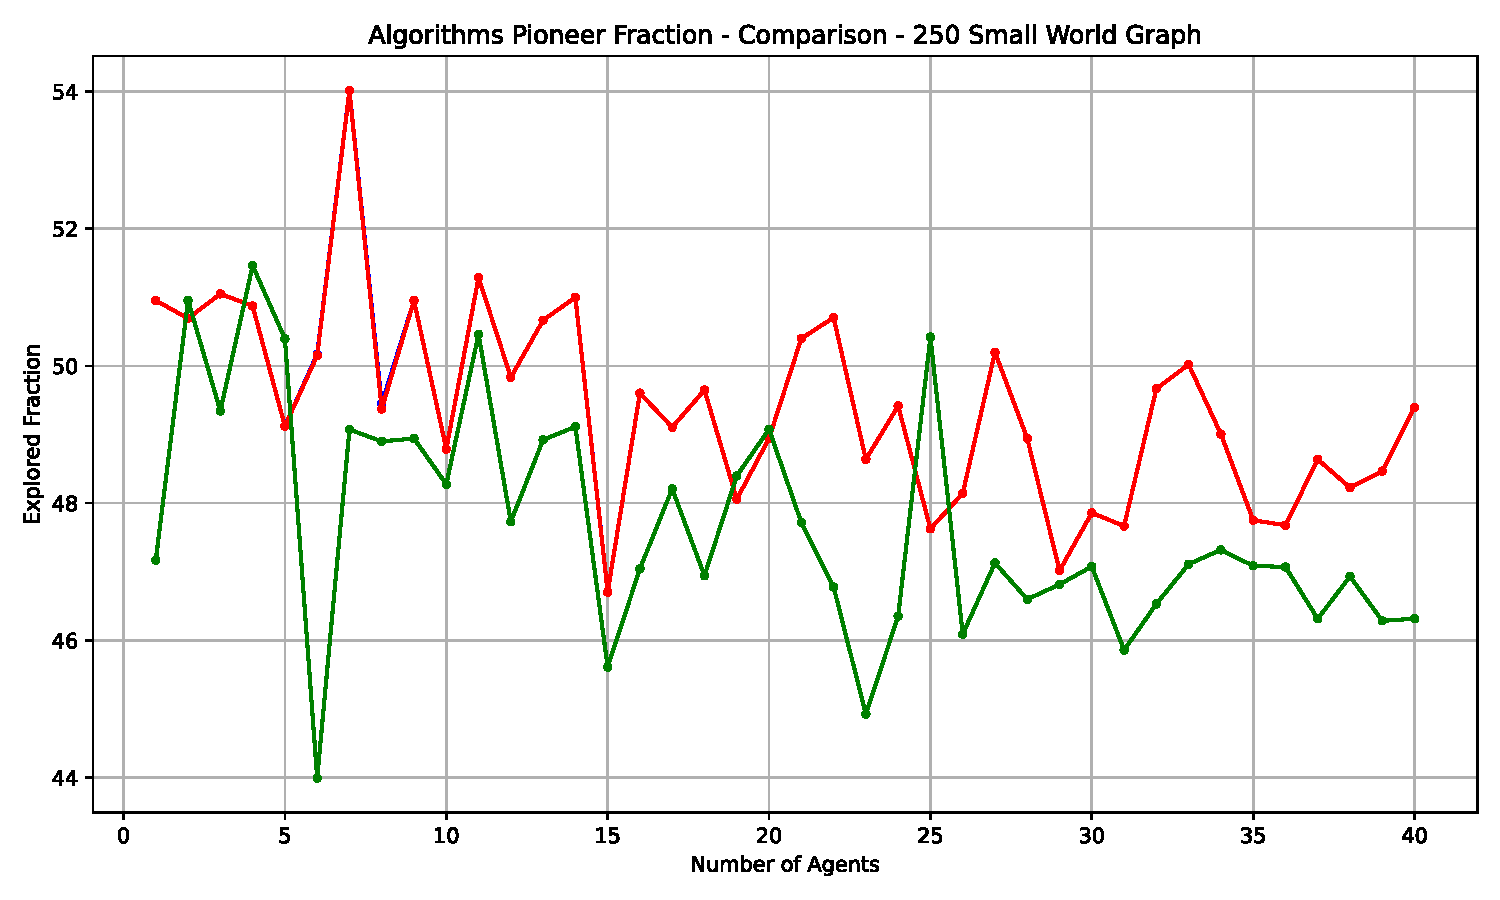
\includegraphics[width=0.45\linewidth]{Cap3/no_comm_fraction__250_sw.pdf} }}
    \newline
    \subfloat[\centering 500-node Small-World]
    {{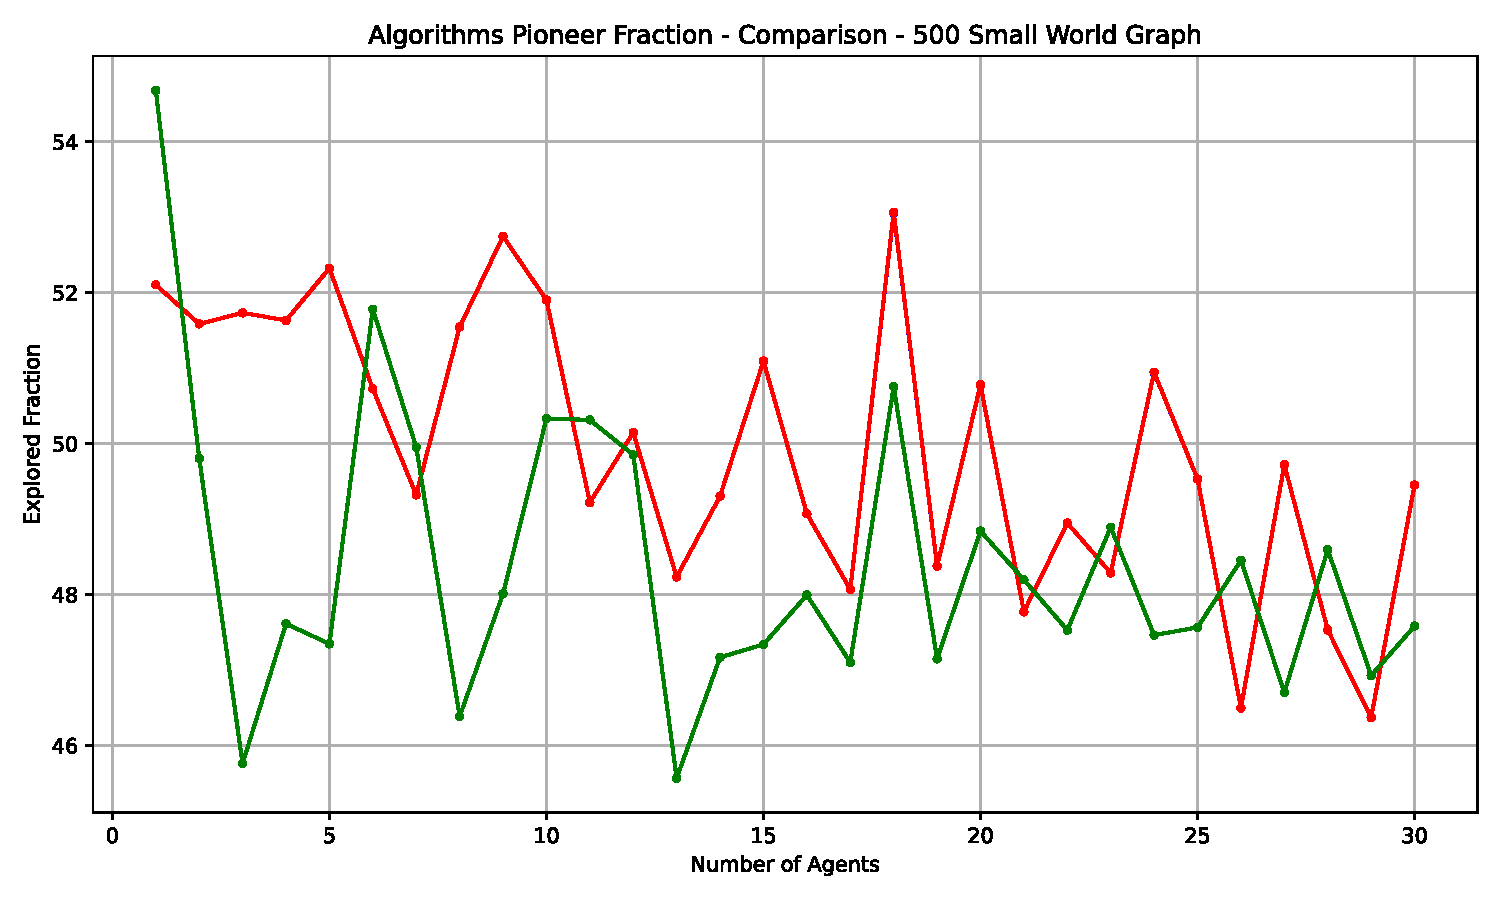
\includegraphics[width=0.45\linewidth]{Cap3/no_comm_fraction__500_sw.pdf} }}
    \qquad
    \subfloat[\centering 1000-node Small-World]
    {{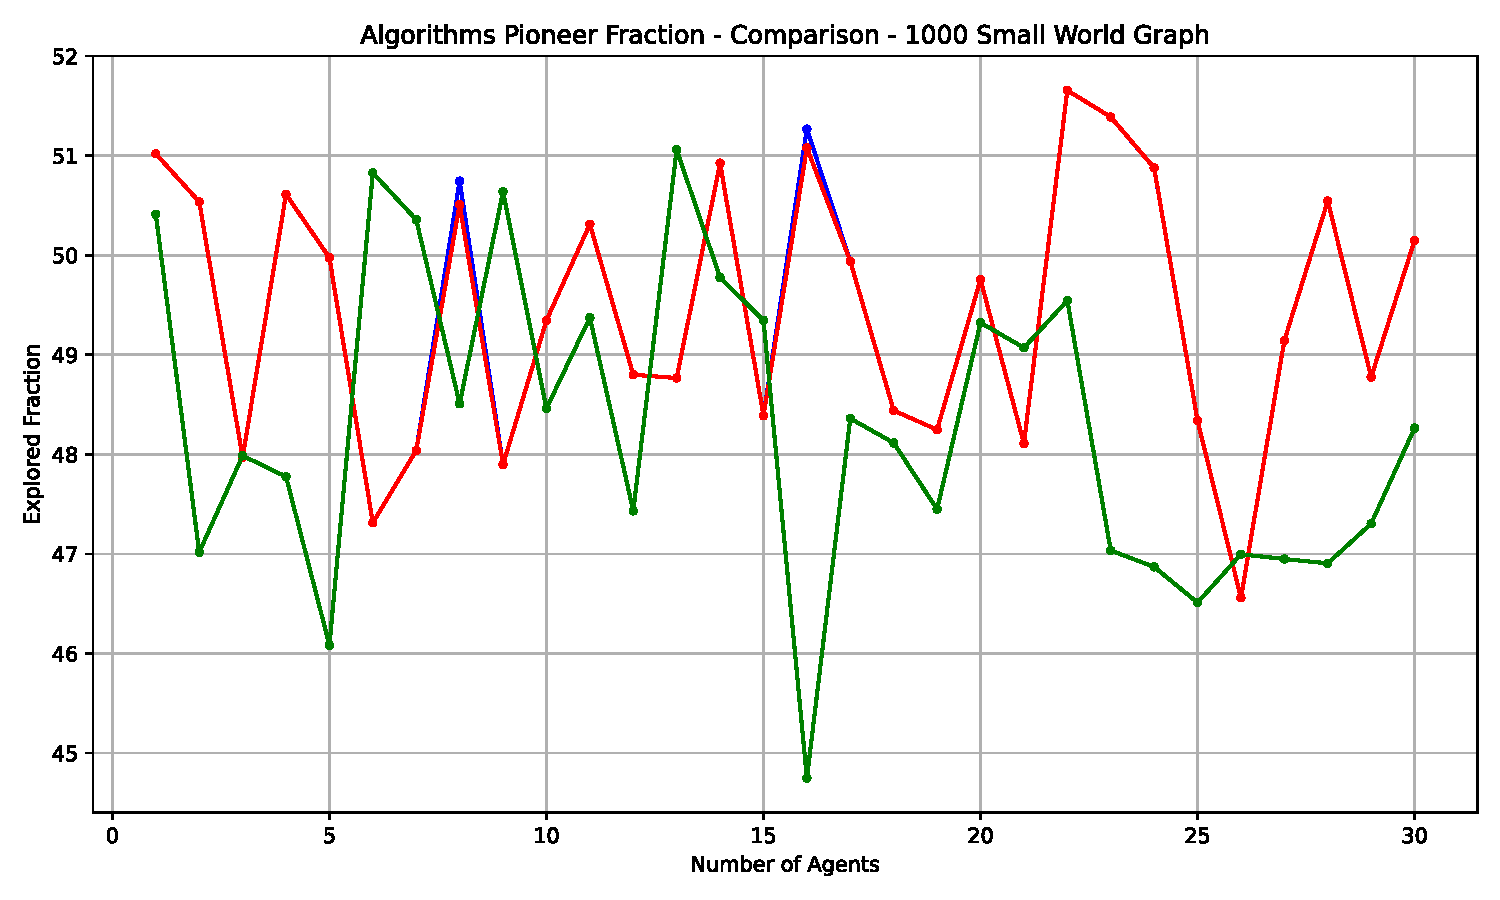
\includegraphics[width=0.45\linewidth]{Cap3/no_comm_fraction__1000_sw.pdf} }}
    \caption{Comparison of the explored fraction achieved by the pioneer across different no-communication algorithms and Tarry's algorithm for various sizes of Small-World graphs. The subfigures illustrate how coverage efficiency varies with graph sizes.}
    \label{fig_no_comm_fraction_all_sizes_sw}
\end{figure}


In Figure \ref{fig_no_comm_steps_all_sizes_sw}, we see a similar trend to Section \ref{subsection_no_comm_barabasi_albert_results}: Tarry's algorithm consistently outperforms the other methods, with performance improving as the number of agents increases, while the Backward Interval Filling algorithm shows no gains over the basic exploration algorithm. This is likely for the same reason as with Barabási-Albert graphs; Small-World graphs are highly connected, and searches often complete before agents finish their assigned intervals. For both graph types, Tarry's algorithm outperforms the no-communication methods by 80.86\% and 84.11\%, respectively, with 30 agents on 1000-node graphs. While Small-World graphs' grid structure could potentially aid dispersion for non-communication algorithms, it seems to enhance Tarry's performance even more, resulting in this observed discrepancy.

In Figure \ref{fig_no_comm_fraction_all_sizes_sw}, which shows the explored fraction before the pioneer reaches the goal, we see similarly noisy results as in Section \ref{subsection_no_comm_random_tree_results}. Tarry's algorithm generally explores a smaller portion of the graph, though the difference is not substantial. This variability likely stems from inconsistent exploration across instances; in some cases, agents must explore a significant portion of the graph to locate the goal, while in others, they explore very little. Tarry's average explored fraction for 1000 nodes with 20 agents is 46.17\%, with a standard deviation of 28.81\%, confirming this inconsistency. Figure \ref{fig_no_comm_fraction_histogram_sw} further illustrates the spread of these exploration results.

\begin{figure}[H]
    \centering 
    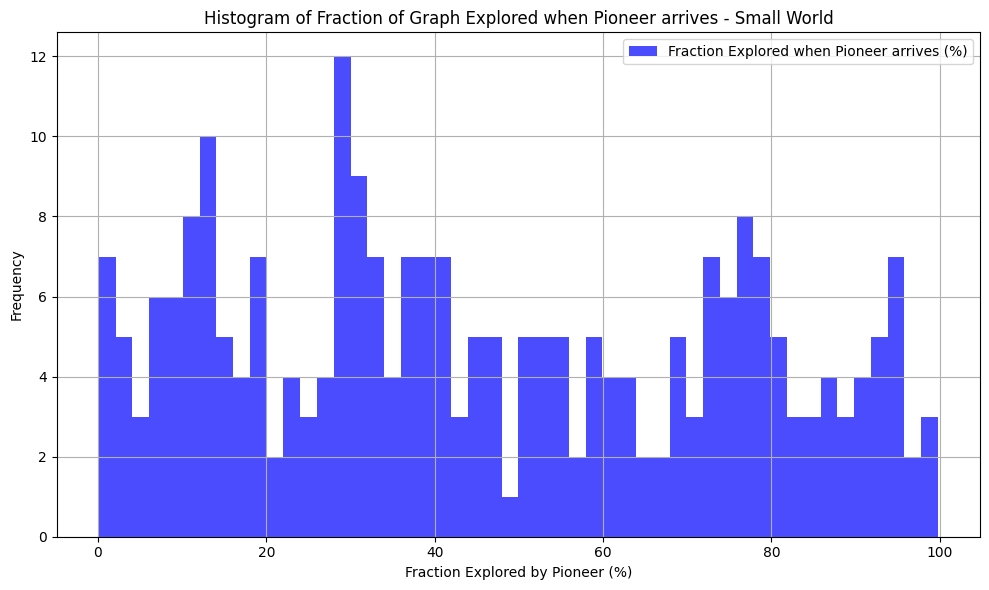
\includegraphics[width=0.7\textwidth]{Cap3/no_comm_fraction_histogram_sw.png} 
    \caption{Histogram of explored fractions for Small World Graphs with 1000 nodes and 20 agents using Tarry's Algorithm.} 
    \label{fig_no_comm_fraction_histogram_sw}
\end{figure}


\section{Tarry's Variants Performance}
\label{section_result_tarry}

\subsection{Metrics for Analysis}
\label{subsection_tarry_metrics}

This section examines the results for Tarry's algorithm and its variants, specifically Tarry Tie-Breaker, Tarry Interval Priority, and Delayed Tarry.

In addition to the previously mentioned metrics in Section \ref{subsection_no_comm_metrics}, this section presents a relative difference in performance compared to the base Tarry algorithm. This approach is particularly useful for interpreting results when the performances of the algorithms are very close on some datasets, as relative values help to better visualize the differences when absolute values are too similar.

\subsection{Perfect Maze Results} 
\label{subsection_tarry_maze_results}

The results for all maze sizes (10x10, 20x20, 30x30, and 40x40) are shown in Figures \ref{fig_tarry_steps_all_sizes_maze}, \ref{fig_tarry_fraction_all_sizes_maze}, and \ref{fig_tarry_steps_relative_all_sizes_maze}, demonstrating the performance of Tarry's algorithm and its variations across different maze dimensions. Figure \ref{fig_tarry_steps_all_sizes_maze} illustrates the number of steps taken by the algorithms, while Figure \ref{fig_tarry_fraction_all_sizes_maze} displays the fraction of the maze explored before reaching the goal, providing insights into exploration efficiency and coverage across maze sizes. Additionally, Figure \ref{fig_tarry_steps_relative_all_sizes_maze} presents the relative difference in pioneer steps compared to the original Tarry's algorithm, helping to better compare the variations, which may show similar behaviors.

\begin{figure}[H]
    \centering
    \qquad
    \qquad
    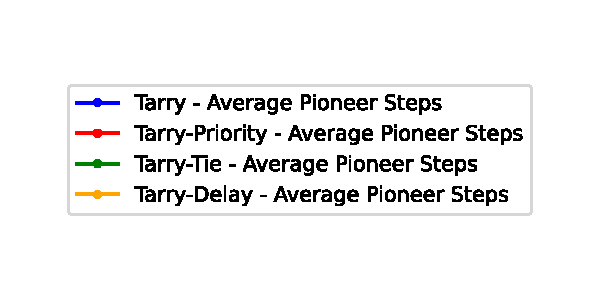
\includegraphics[width=0.5\textwidth]{Cap3/tarry_var_steps_legend.pdf}
    \newline
    \subfloat[\centering 10x10 Maze]
    {{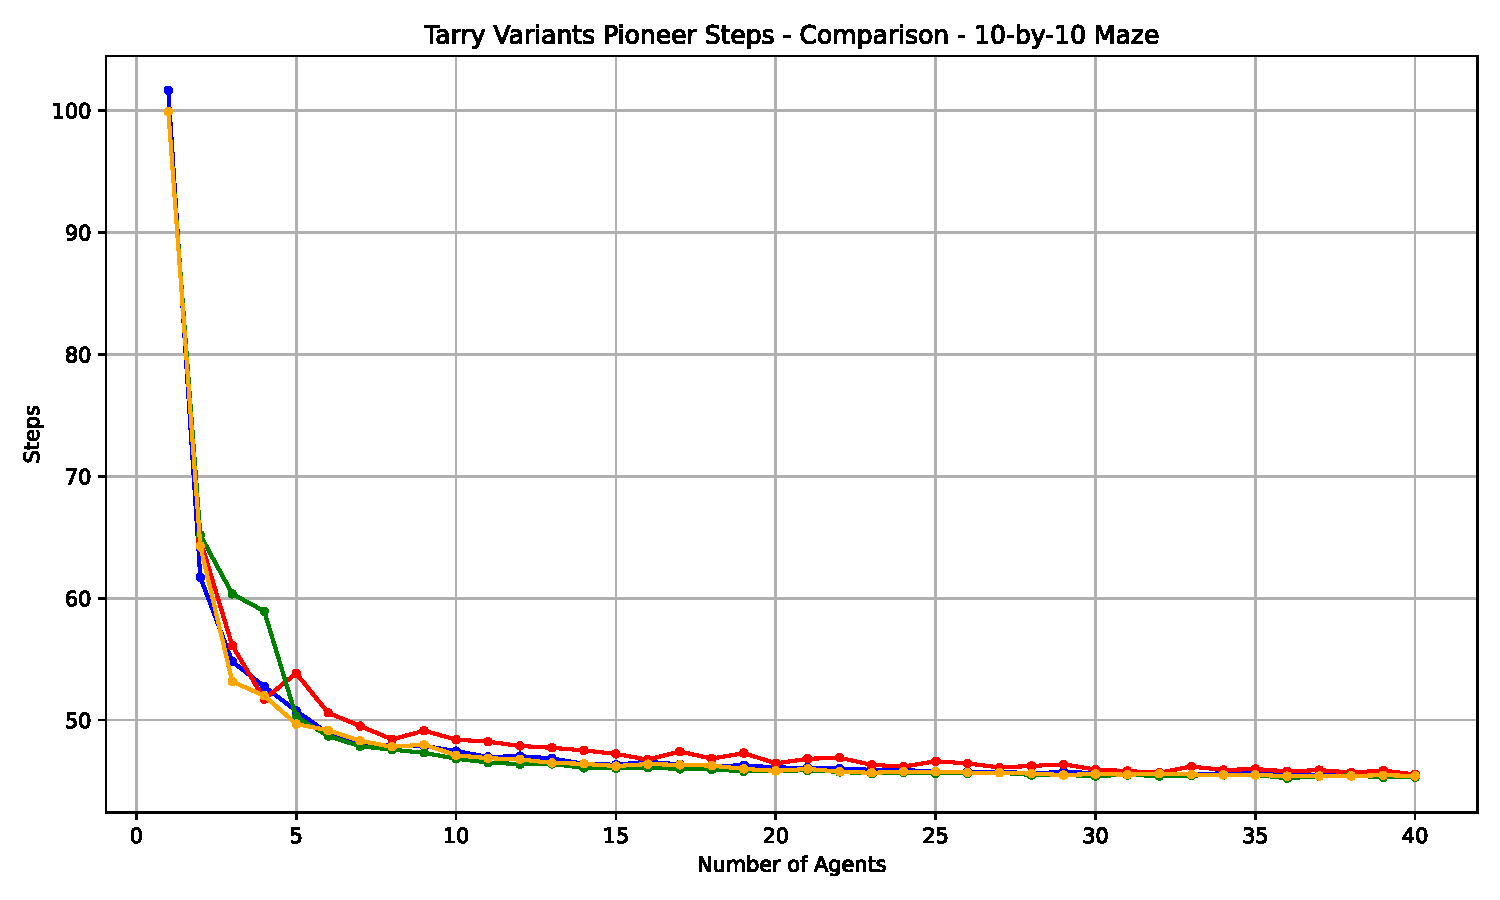
\includegraphics[width=0.45\linewidth]{Cap3/tarry_var_steps__10_by_10_maze.pdf} }}
    \qquad
    \subfloat[\centering 20x20 Maze]
    {{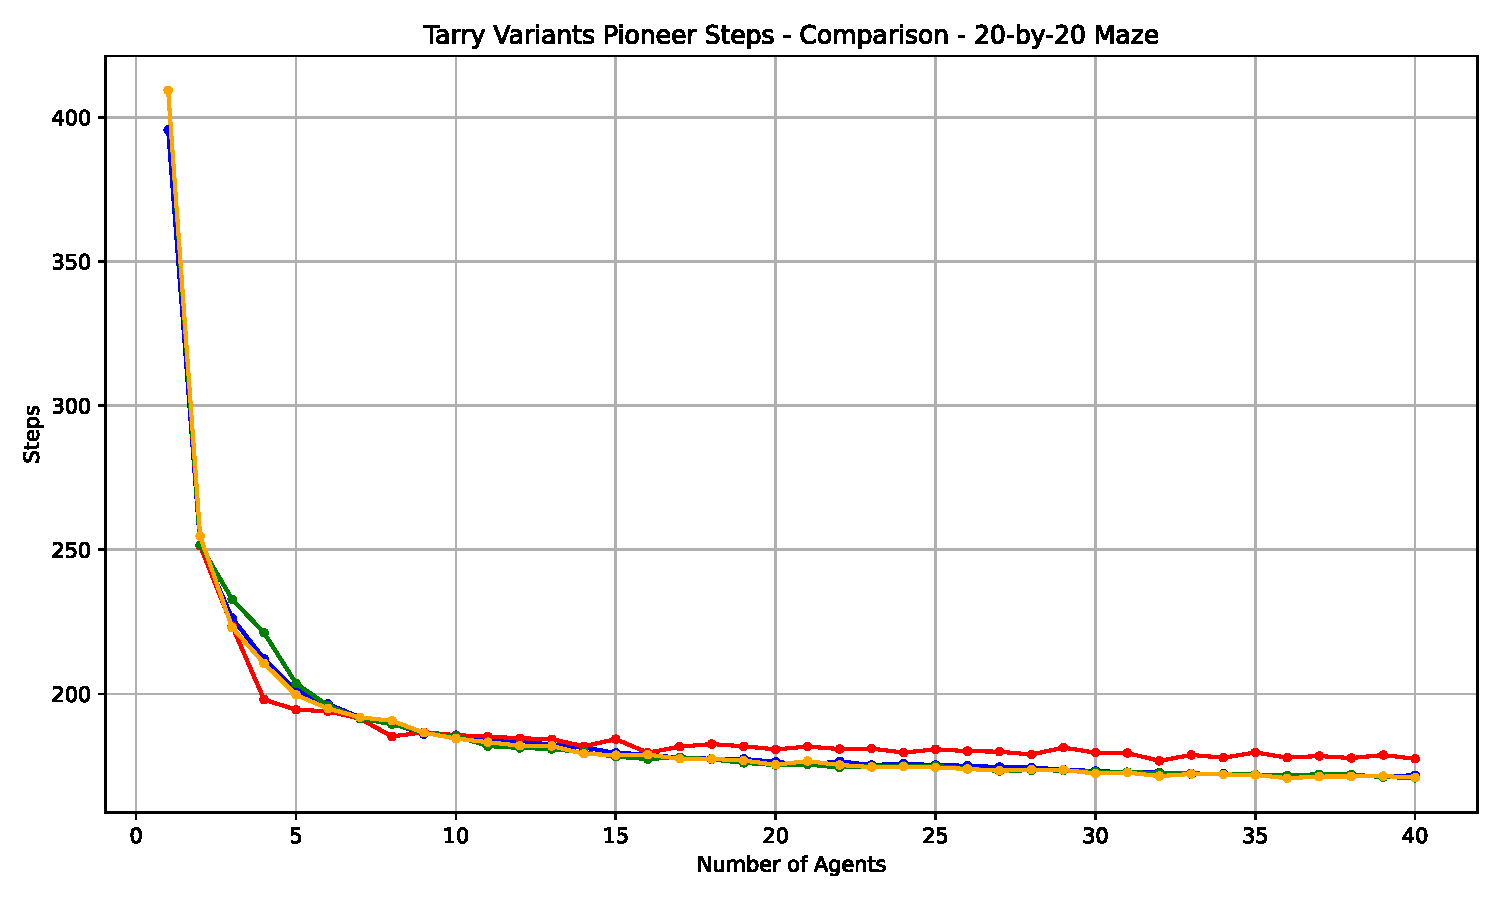
\includegraphics[width=0.45\linewidth]{Cap3/tarry_var_steps__20_by_20_maze.pdf} }}
    \newline
    \subfloat[\centering 30x30 Maze]
    {{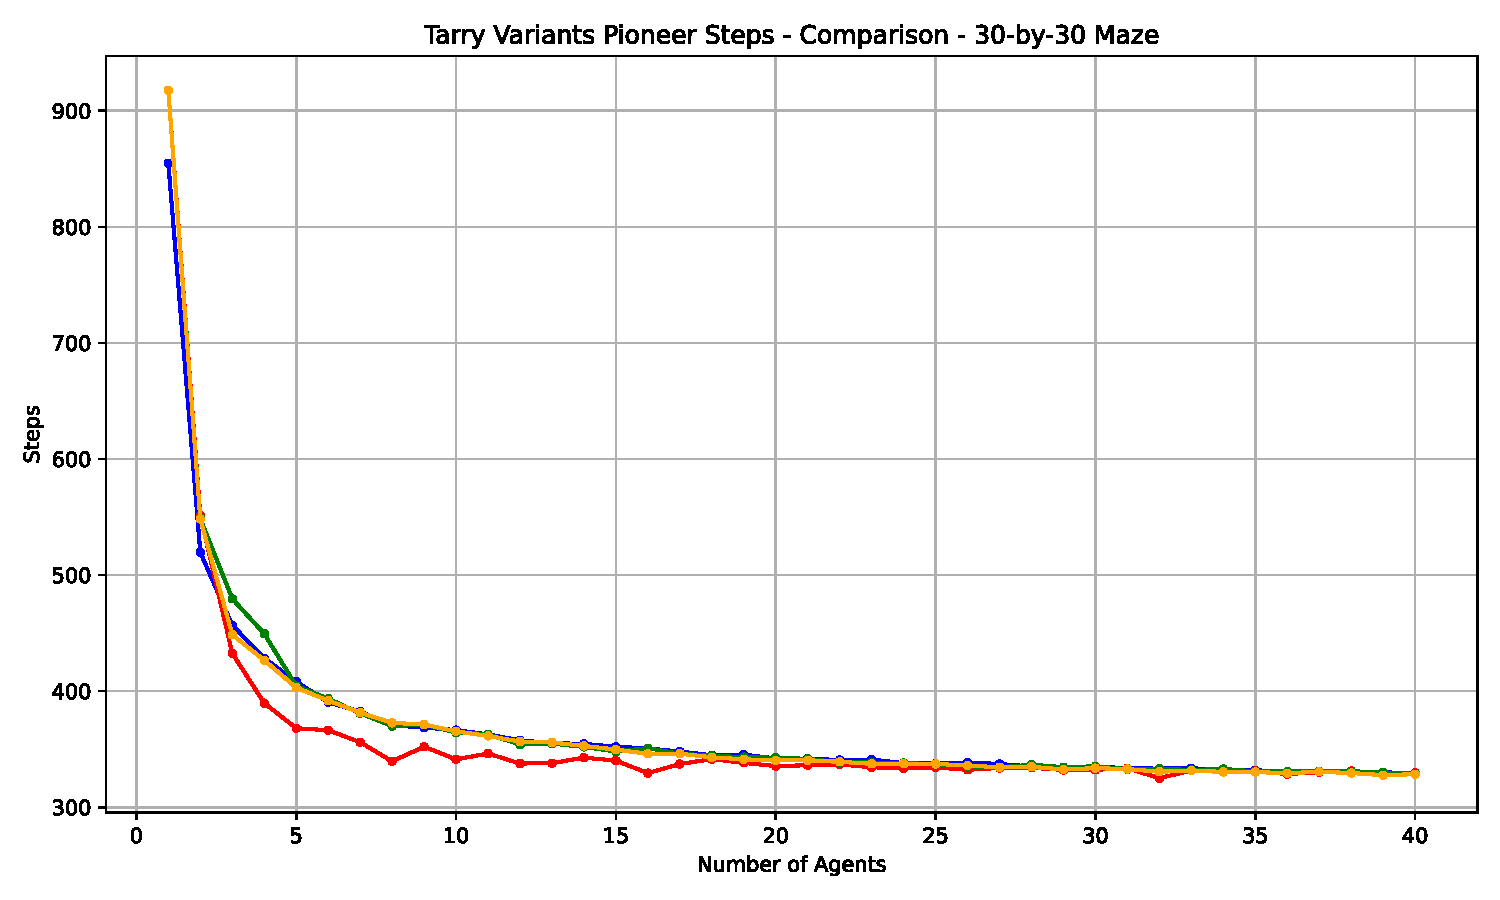
\includegraphics[width=0.45\linewidth]{Cap3/tarry_var_steps__30_by_30_maze.pdf} }}
    \qquad
    \subfloat[\centering 40x40 Maze]
    {{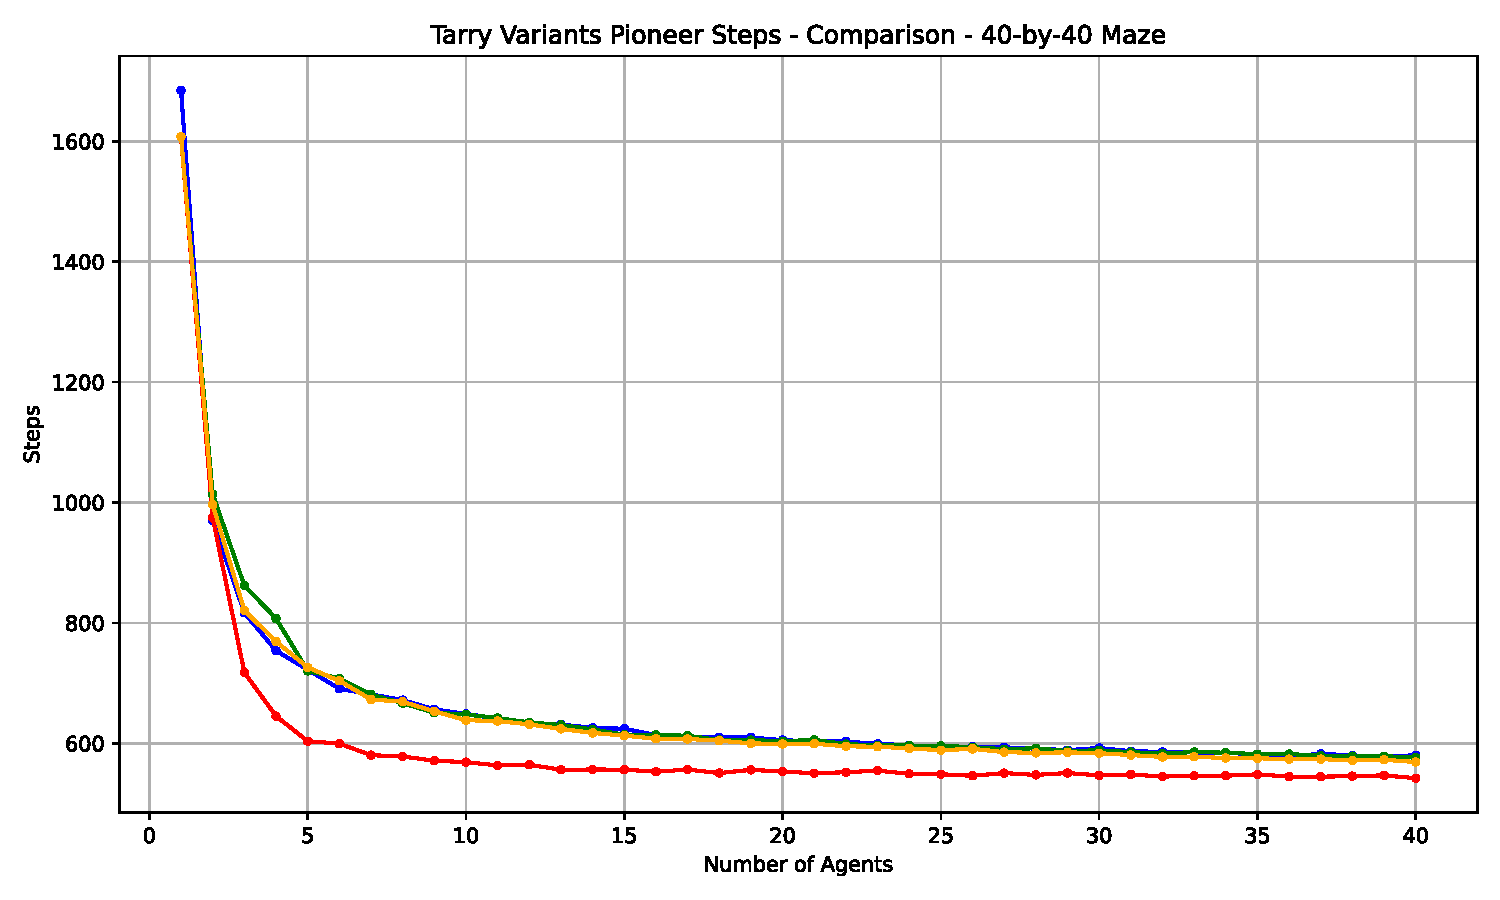
\includegraphics[width=0.45\linewidth]{Cap3/tarry_var_steps__40_by_40_maze.pdf} }}
    \caption{Comparison of the pioneer's average steps across Tarry's algorithm and its variations for different sizes of perfect mazes. The subfigures illustrate how algorithm performance changes with maze size.}
    \label{fig_tarry_steps_all_sizes_maze}
\end{figure}

\begin{figure}[H]
    \centering
    \qquad
    \qquad
    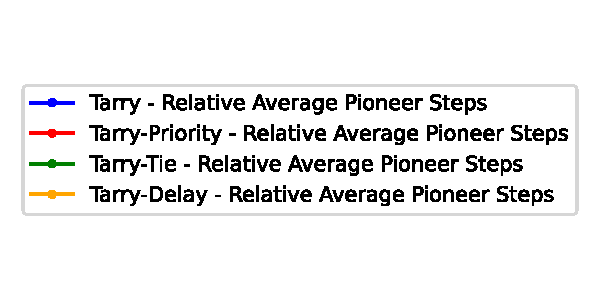
\includegraphics[width=0.5\textwidth]{Cap3/tarry_var_steps_legend_relative.pdf}
    \newline
    \subfloat[\centering 10x10 Maze]
    {{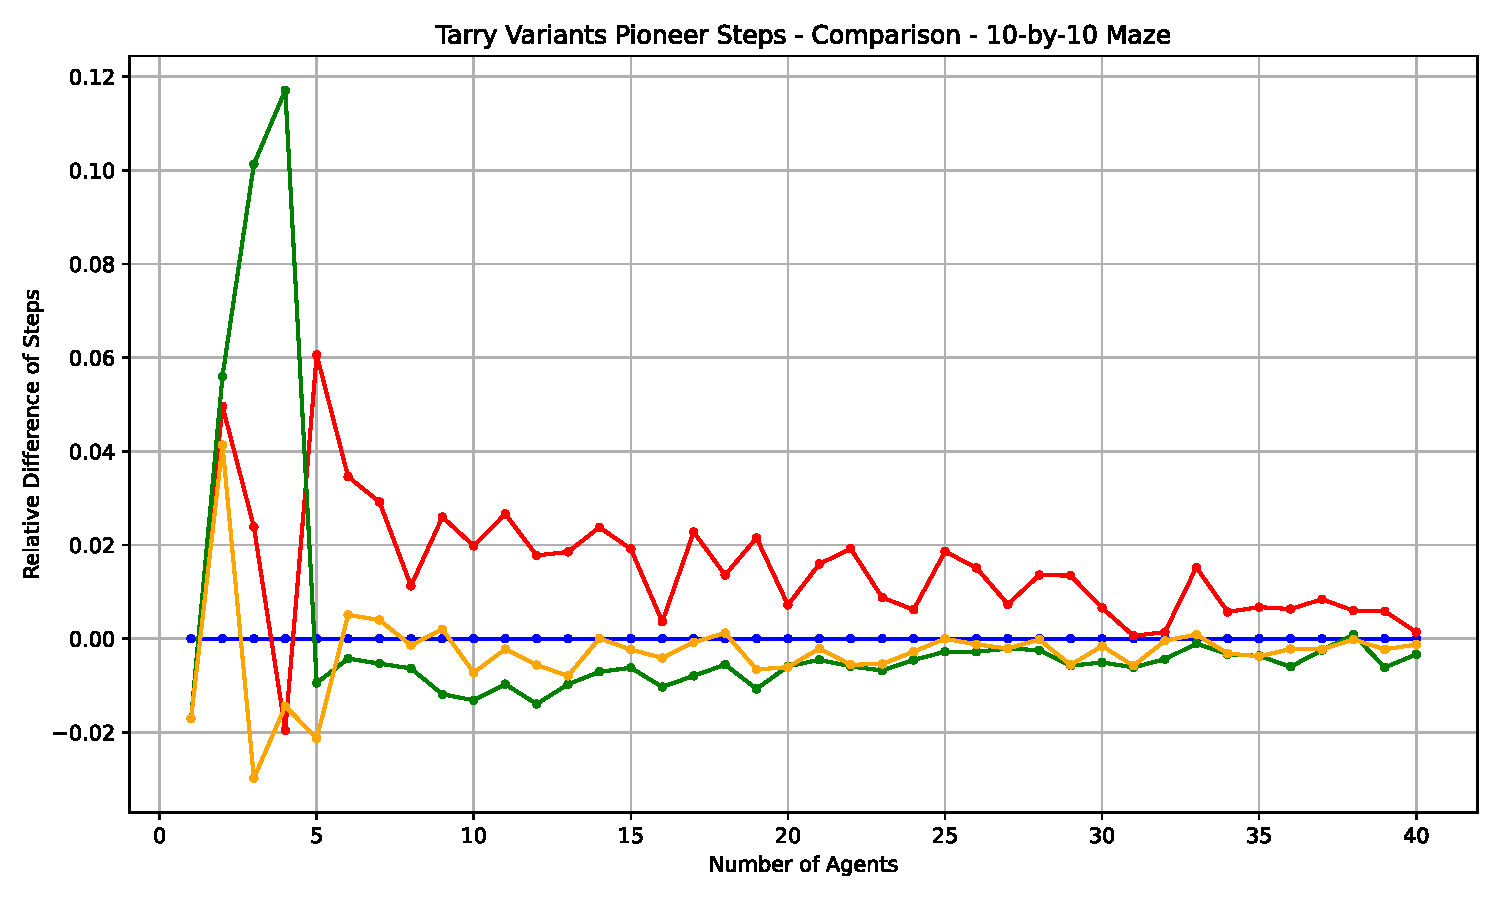
\includegraphics[width=0.45\linewidth]{Cap3/tarry_var_steps__10_by_10_maze_relative.pdf} }}
    \qquad
    \subfloat[\centering 20x20 Maze]
    {{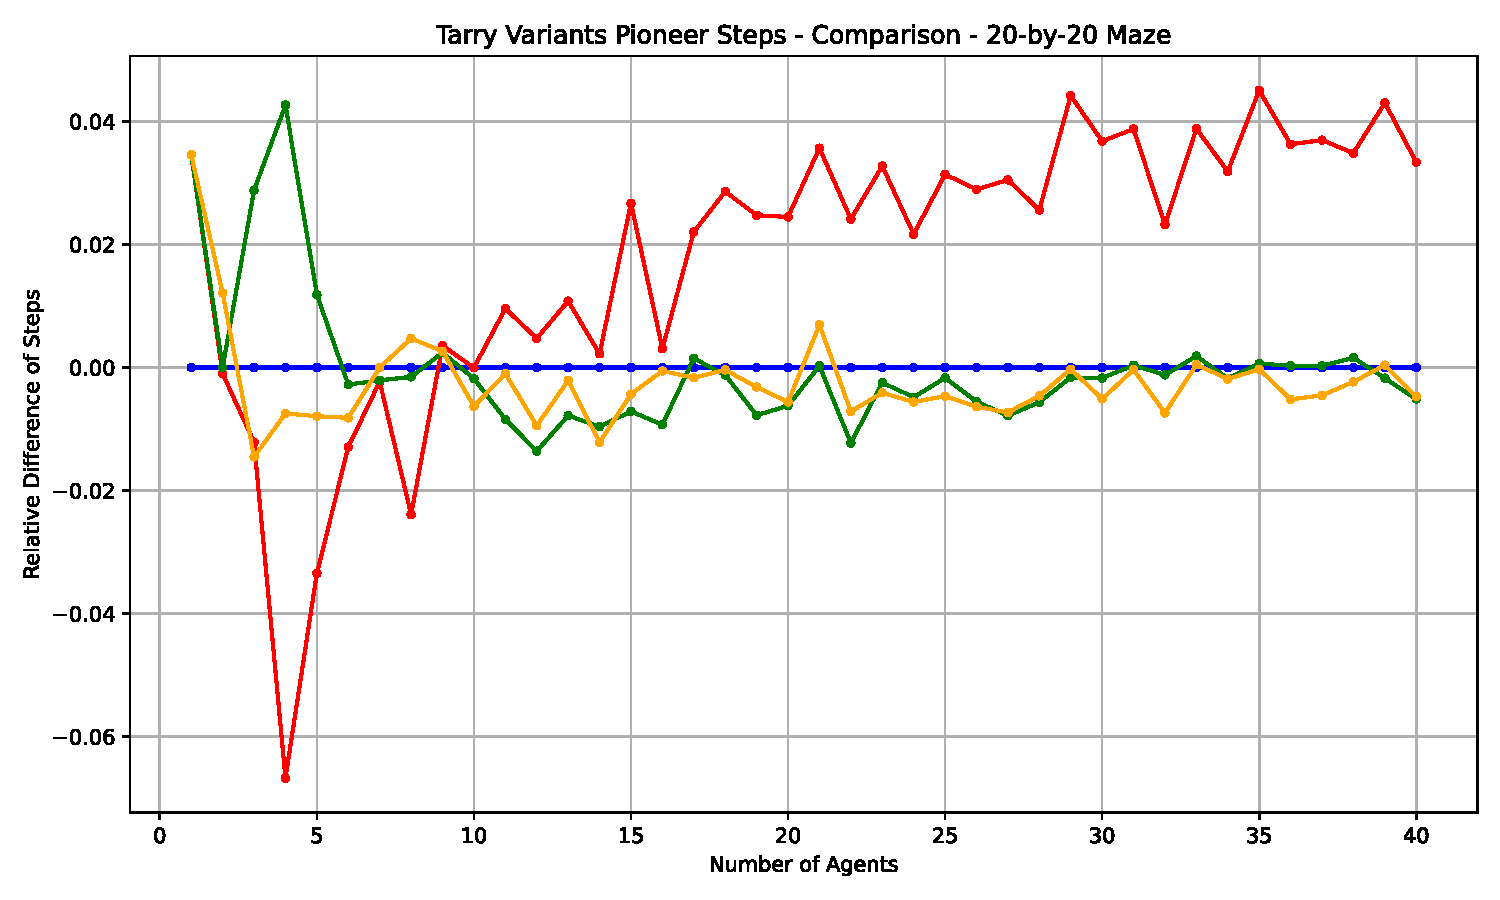
\includegraphics[width=0.45\linewidth]{Cap3/tarry_var_steps__20_by_20_maze_relative.pdf} }}
    \newline
    \subfloat[\centering 30x30 Maze]
    {{\includegraphics[width=0.45\linewidth]{Cap3/tarry_var_steps__30_by_30_maze_relative.pdf} }}
    \qquad
    \subfloat[\centering 40x40 Maze]
    {{\includegraphics[width=0.45\linewidth]{Cap3/tarry_var_steps__40_by_40_maze_relative.pdf} }}
    \caption{Relative difference in pioneer steps between Tarry's algorithm variants and the original Tarry's algorithm, across different sizes of perfect mazes. The subfigures illustrate how the relative performance changes with maze size.}
    \label{fig_tarry_steps_relative_all_sizes_maze}
\end{figure}

\begin{figure}[H]
    \centering
    \qquad
    \qquad
    \includegraphics[width=0.5\textwidth]{Cap3/tarry_var_fraction_legend.pdf}
    \newline
    \subfloat[\centering 10x10 Maze]
    {{\includegraphics[width=0.45\linewidth]{Cap3/tarry_var_fraction__10_by_10_maze.pdf} }}
    \qquad
    \subfloat[\centering 20x20 Maze]
    {{\includegraphics[width=0.45\linewidth]{Cap3/tarry_var_fraction__20_by_20_maze.pdf} }}
    \newline
    \subfloat[\centering 30x30 Maze]
    {{\includegraphics[width=0.45\linewidth]{Cap3/tarry_var_fraction__30_by_30_maze.pdf} }}
    \qquad
    \subfloat[\centering 40x40 Maze]
    {{\includegraphics[width=0.45\linewidth]{Cap3/tarry_var_fraction__40_by_40_maze.pdf} }}
    \caption{Comparison of the explored fraction across Tarry's algorithm and its variations for different sizes of perfect mazes. The subfigures illustrate how the explored fraction changes with maze size.}
    \label{fig_tarry_fraction_all_sizes_maze}
\end{figure}
 
When analyzing Figures \ref{fig_tarry_steps_all_sizes_maze} and \ref{fig_tarry_steps_relative_all_sizes_maze}, it becomes evident that there is no uniform trend across all maze sizes. The Tarry Tie-Breaker and Delayed Tarry variations consistently outperform the standard Tarry algorithm, except in cases with a small number of agents. In those cases, early variations in exploration paths can significantly affect the outcome due to the extensive search required by each agent. However, a more intriguing behavior is observed with the Tarry Interval Priority variation. Although it performs similarly but slightly worse for smaller maze sizes, its performance improves for the largest maze analyzed. We conjecture this behavior can be attributed to the benefits of dispersion and the additional information obtained through interval filling, which only becomes significant during more extensive exploration. In mazes with considerable depth and narrow width, we believe interval filling initially causes conflicts, as agents may search for the start of their intervals in branches that have already been visited by others. However, in larger mazes, we assume these initial setbacks are offset by the advantages gained through the extra information during deeper exploration, which cannot be easily matched by Tarry's random choices.


An interesting observation can also be made regarding the explored fraction, as shown in Figure \ref{fig_tarry_fraction_all_sizes_maze}. The results indicate that the Tarry Interval Priority algorithm consistently explores a smaller portion of the graph compared to the other variations. Since mazes have few leaf nodes and communication prevents agents from overlapping in explored branches, the use of intervals likely directs agents more efficiently toward unexplored areas, potentially allowing them to head directly to leaf nodes before finding the actual solution.


\subsection{Random Tree Results} 
\label{subsection_tarry_random_tree_results}


The results for the random trees, using the same sizes as in Section \ref{subsection_no_comm_random_tree_results}, are presented in Figures \ref{fig_tarry_steps_all_sizes_tree}, \ref{fig_tarry_fraction_all_sizes_tree}, and \ref{fig_tarry_steps_relative_all_sizes_tree}.

\begin{figure}[H]
    \centering
    \qquad
    \qquad
    \includegraphics[width=0.5\textwidth]{Cap3/tarry_var_steps_legend.pdf}
    \newline
    \subfloat[\centering 100-node Tree]
    {{\includegraphics[width=0.45\linewidth]{Cap3/tarry_var_steps__100_tree.pdf} }}
    \qquad
    \subfloat[\centering 500-node Tree]
    {{\includegraphics[width=0.45\linewidth]{Cap3/tarry_var_steps__500_tree.pdf} }}
    \newline
    \subfloat[\centering 1000-node Tree]
    {{\includegraphics[width=0.45\linewidth]{Cap3/tarry_var_steps__1000_tree.pdf} }}
    \qquad
    \subfloat[\centering 1500-node Tree]
    {{\includegraphics[width=0.45\linewidth]{Cap3/tarry_var_steps__1500_tree.pdf} }} 
    \caption{Comparison of the pioneer's average steps across Tarry's algorithm and its variations for different sizes of random trees. The subfigures illustrate how algorithm performance changes with tree size.} 
    \label{fig_tarry_steps_all_sizes_tree} 
\end{figure}

\begin{figure}[H]
    \centering
    \qquad
    \qquad
    \includegraphics[width=0.5\textwidth]{Cap3/tarry_var_steps_legend_relative.pdf}
    \newline
    \subfloat[\centering 100-node Tree]
    {{\includegraphics[width=0.45\linewidth]{Cap3/tarry_var_steps__100_tree_relative.pdf} }}
    \qquad 
    \subfloat[\centering 500-node Tree]
    {{\includegraphics[width=0.45\linewidth]{Cap3/tarry_var_steps__500_tree_relative.pdf} }}
    \newline
    \subfloat[\centering 1000-node Tree]
    {{\includegraphics[width=0.45\linewidth]{Cap3/tarry_var_steps__1000_tree_relative.pdf} }}
    \qquad 
    \subfloat[\centering 1500-node Tree]
    {{\includegraphics[width=0.45\linewidth]{Cap3/tarry_var_steps__1500_tree_relative.pdf} }} 
    \caption{Relative difference in pioneer steps between Tarry's algorithm variants and the original Tarry's algorithm across different sizes of random trees. The subfigures illustrate how the relative performance changes with tree size.} 
    \label{fig_tarry_steps_relative_all_sizes_tree}
\end{figure}

\begin{figure}[H]
    \centering
    \qquad
    \qquad
    \includegraphics[width=0.5\textwidth]{Cap3/tarry_var_fraction_legend.pdf} 
    \newline 
    \subfloat[\centering 100-node Tree]
    {{\includegraphics[width=0.45\linewidth]{Cap3/tarry_var_fraction__100_tree.pdf} }}
    \qquad
    \subfloat[\centering 500-node Tree]
    {{\includegraphics[width=0.45\linewidth]{Cap3/tarry_var_fraction__500_tree.pdf} }}
    \newline 
    \subfloat[\centering 1000-node Tree]
    {{\includegraphics[width=0.45\linewidth]{Cap3/tarry_var_fraction__1000_tree.pdf} }}
    \qquad
    \subfloat[\centering 1500-node Tree]
    {{\includegraphics[width=0.45\linewidth]{Cap3/tarry_var_fraction__1500_tree.pdf} }}
    \caption{Comparison of the explored fraction across Tarry's algorithm and its variations for different sizes of random trees. The subfigures illustrate how the explored fraction changes with tree size.} 
    \label{fig_tarry_fraction_all_sizes_tree} 
\end{figure}

According to Figures \ref{fig_tarry_steps_all_sizes_tree} and \ref{fig_tarry_steps_relative_all_sizes_tree}, the results show a distinct pattern compared to those observed in Section \ref{subsection_tarry_maze_results}. The Tarry Interval Priority variation consistently underperforms across all tree sizes, with the disparity becoming even more pronounced when the number of agents is small. This outcome is likely due to the wide structure of the trees, where each agent in this variation needs to explore many leaf nodes within its assigned interval, resulting in inefficiencies. In contrast, only the Tarry Tie-Breaker shows small but consistent improvement for smaller number of nodes, although this advantage tends to disappear for larger trees.


When examining Figure \ref{fig_tarry_fraction_all_sizes_tree}, a similar behavior to what was previously discussed in Figure \ref{fig_no_comm_fraction_all_sizes_tree} can be observed. The explored fraction displays a pattern that is largely independent of the strategy used, due to the high variability in the fraction of nodes explored across different tree instances.

\subsection{Barabási-Albert Results} 
\label{subsection_tarry_barabasi_albert_results}

The results for the Barabási-Albert graphs, using the same sizes as in Section \ref{subsection_no_comm_barabasi_albert_results}, are presented in Figures \ref{fig_tarry_steps_all_sizes_barabasi}, \ref{fig_tarry_fraction_all_sizes_barabasi}, and \ref{fig_tarry_steps_relative_all_sizes_barabasi}.


\begin{figure}[H]
    \centering
    \qquad
    \qquad
    \includegraphics[width=0.5\textwidth]{Cap3/tarry_var_steps_legend.pdf}
    \newline
    \subfloat[\centering 100-node Barabási-Albert]
    {{\includegraphics[width=0.45\linewidth]{Cap3/tarry_var_steps__100_barabasi.pdf} }}
    \qquad
    \subfloat[\centering 250-node Barabási-Albert]
    {{\includegraphics[width=0.45\linewidth]{Cap3/tarry_var_steps__250_barabasi.pdf} }}
    \newline
    \subfloat[\centering 500-node Barabási-Albert]
    {{\includegraphics[width=0.45\linewidth]{Cap3/tarry_var_steps__500_barabasi.pdf} }}
    \qquad
    \subfloat[\centering 1000-node Barabási-Albert]
    {{\includegraphics[width=0.45\linewidth]{Cap3/tarry_var_steps__1000_barabasi.pdf} }} 
    \caption{Comparison of the pioneer's average steps across Tarry's algorithm and its variations for different sizes of Barabási-Albert graphs. The subfigures illustrate how algorithm performance changes with graph size.} 
    \label{fig_tarry_steps_all_sizes_barabasi} 
\end{figure}


\begin{figure}[H]
    \centering
    \qquad
    \qquad
    \includegraphics[width=0.5\textwidth]{Cap3/tarry_var_steps_legend_relative.pdf}
    \newline
    \subfloat[\centering 100-node Barabási-Albert]
    {{\includegraphics[width=0.45\linewidth]{Cap3/tarry_var_steps__100_barabasi_relative.pdf} }}
    \qquad 
    \subfloat[\centering 250-node Barabási-Albert]
    {{\includegraphics[width=0.45\linewidth]{Cap3/tarry_var_steps__250_barabasi_relative.pdf} }}
    \newline
    \subfloat[\centering 500-node Barabási-Albert]
    {{\includegraphics[width=0.45\linewidth]{Cap3/tarry_var_steps__500_barabasi_relative.pdf} }}
    \qquad
    \subfloat[\centering 1000-node Barabási-Albert]
    {{\includegraphics[width=0.45\linewidth]{Cap3/tarry_var_steps__1000_barabasi_relative.pdf} }} 
    \caption{Relative difference in pioneer steps between Tarry's algorithm variants and the original Tarry's algorithm across different sizes of Barabási-Albert graphs. The subfigures illustrate how the relative performance changes with graph size.} 
    \label{fig_tarry_steps_relative_all_sizes_barabasi}
\end{figure}

\begin{figure}[H]
    \centering
    \qquad
    \qquad
    \includegraphics[width=0.5\textwidth]{Cap3/tarry_var_fraction_legend.pdf}
    \newline 
    \subfloat[\centering 100-node Barabási-Albert]
    {{\includegraphics[width=0.45\linewidth]{Cap3/tarry_var_fraction__100_barabasi.pdf} }}
    \qquad
    \subfloat[\centering 250-node Barabási-Albert]
    {{\includegraphics[width=0.45\linewidth]{Cap3/tarry_var_fraction__250_barabasi.pdf} }}
    \newline 
    \subfloat[\centering 500-node Barabási-Albert]
    {{\includegraphics[width=0.45\linewidth]{Cap3/tarry_var_fraction__500_barabasi.pdf} }}
    \qquad
    \subfloat[\centering 1000-node Barabási-Albert]
    {{\includegraphics[width=0.45\linewidth]{Cap3/tarry_var_fraction__1000_barabasi.pdf} }}
    \caption{Comparison of the explored fraction across Tarry's algorithm and its variations for different sizes of Barabási-Albert graphs. The subfigures illustrate how the explored fraction changes with graph size.} 
    \label{fig_tarry_fraction_all_sizes_barabasi} 
\end{figure}

Examining Figures \ref{fig_tarry_steps_all_sizes_barabasi} and \ref{fig_tarry_steps_relative_all_sizes_barabasi}, the poorer performance of the Tarry Interval Priority variation stands out. The results closely resemble those from the no-communication algorithms in \ref{subsection_no_comm_barabasi_albert_results}, likely due to the high connectivity in Barabási-Albert graphs. This structure accelerates exploration, often completing before an agent exhausts its interval, thus yielding similar outcomes.

Additionally, while the Tie-Breaker and Delayed Tarry variations perform worse than base Tarry on smaller datasets, they tend to improve, becoming consistently comparable or slightly superior as graph size increases.

As expected, the explored fraction of the graph before the pioneer reaches the goal shows the same downward trend observed in \ref{subsection_no_comm_barabasi_albert_results}, with a smaller explored fraction as more agents are added. For larger Barabási-Albert graphs, the choice of algorithm has little impact on the explored fraction; however, for the smaller 100-node graph, Tarry's and the Tarry Tie-Breaker variation tend to explore less.
    
\subsection{Small-World Results} 
\label{subsection_tarry_sw_results}

The results for Small-World graphs, using the same sizes as in Section \ref{subsection_no_comm_sw_results} are presented in Figures \ref{fig_tarry_steps_all_sizes_sw}, \ref{fig_tarry_steps_relative_all_sizes_sw}, and \ref{fig_tarry_fraction_all_sizes_sw}.

\begin{figure}[H]
    \centering
    \qquad
    \qquad
    \includegraphics[width=0.5\textwidth]{Cap3/tarry_var_steps_legend.pdf}
    \newline
    \subfloat[\centering 100-node Small-World]
    {{\includegraphics[width=0.45\linewidth]{Cap3/tarry_var_steps__100_sw.pdf} }}
    \qquad
    \subfloat[\centering 250-node Small-World]
    {{\includegraphics[width=0.45\linewidth]{Cap3/tarry_var_steps__250_sw.pdf} }}
    \newline
    \subfloat[\centering 500-node Small-World]
    {{\includegraphics[width=0.45\linewidth]{Cap3/tarry_var_steps__500_sw.pdf} }}
    \qquad
    \subfloat[\centering 1000-node Small-World]
    {{\includegraphics[width=0.45\linewidth]{Cap3/tarry_var_steps__1000_sw.pdf} }} 
    \caption{Comparison of the pioneer's average steps across Tarry's algorithm and its variations for different sizes of Small-World graphs. The subfigures illustrate how algorithm performance changes with graph size.} 
    \label{fig_tarry_steps_all_sizes_sw} 
\end{figure}

\begin{figure}[H]
    \centering
    \qquad
    \qquad
    \includegraphics[width=0.5\textwidth]{Cap3/tarry_var_steps_legend_relative.pdf}
    \newline
    \subfloat[\centering 100-node Small-World]
    {{\includegraphics[width=0.45\linewidth]{Cap3/tarry_var_steps__100_sw_relative.pdf} }}
    \qquad 
    \subfloat[\centering 250-node Small-World]
    {{\includegraphics[width=0.45\linewidth]{Cap3/tarry_var_steps__250_sw_relative.pdf} }}
    \newline
    \subfloat[\centering 500-node Small-World]
    {{\includegraphics[width=0.45\linewidth]{Cap3/tarry_var_steps__500_sw_relative.pdf} }}
    \qquad
    \subfloat[\centering 1000-node Small-World]
    {{\includegraphics[width=0.45\linewidth]{Cap3/tarry_var_steps__1000_sw_relative.pdf} }} 
    \caption{Relative difference in pioneer steps between Tarry's algorithm variants and the original Tarry's algorithm across different sizes of Small-World graphs. The subfigures illustrate how the relative performance changes with graph size.} 
    \label{fig_tarry_steps_relative_all_sizes_sw}
\end{figure}

\begin{figure}[H]
    \centering
    \qquad
    \qquad
    \includegraphics[width=0.5\textwidth]{Cap3/tarry_var_fraction_legend.pdf}
    \newline 
    \subfloat[\centering 100-node Small-World]
    {{\includegraphics[width=0.45\linewidth]{Cap3/tarry_var_fraction__100_sw.pdf} }}
    \qquad
    \subfloat[\centering 250-node Small-World]
    {{\includegraphics[width=0.45\linewidth]{Cap3/tarry_var_fraction__250_sw.pdf} }}
    \newline 
    \subfloat[\centering 500-node Small-World]
    {{\includegraphics[width=0.45\linewidth]{Cap3/tarry_var_fraction__500_sw.pdf} }}
    \qquad
    \subfloat[\centering 1000-node Small-World]
    {{\includegraphics[width=0.45\linewidth]{Cap3/tarry_var_fraction__1000_sw.pdf} }}
    \caption{Comparison of the explored fraction across Tarry's algorithm and its variations for different sizes of Small-World graphs. The subfigures illustrate how the explored fraction changes with graph size.} 
    \label{fig_tarry_fraction_all_sizes_sw} 
\end{figure}

In analyzing the results in Figures \ref{fig_tarry_steps_all_sizes_sw} and \ref{fig_tarry_steps_relative_all_sizes_sw}, we find that the Tarry Interval Priority variation performs poorly. This is likely due to agents not completing their intervals, similar to the Backward Interval Filling results, which yield outcomes akin to the base exploration algorithm in Figure \ref{fig_no_comm_steps_all_sizes_sw}. Furthermore, the other variations show reduced performance on smaller datasets, while their influence is negligible in the largest dataset, where all methods yield comparable results. These findings suggest that the added complexity does not enhance performance; Tarry's algorithm disperses effectively enough that heuristics are unnecessary for finding the goal quickly. For instance, the average number of steps for the pioneer in the 1000-node case is around 27, which is just 2.7\% of the total number of nodes.

Examining the explored fraction in Figure \ref{fig_tarry_fraction_all_sizes_sw}, we observe a similarly noisy behavior to that seen in Figure \ref{fig_no_comm_fraction_all_sizes_sw}. The explored fraction demonstrates considerable variability across instances, regardless of the variation applied. This indicates that there is no dominant solution for this metric, reflecting the inconsistency in exploration outcomes.